%QQQ Below: "10pt" prints in 10-point. "12pt" prints in larger 12-point.
\documentclass[12pt,letterpaper]{article}
\usepackage{amsthm,amssymb,amsmath}
\usepackage[pdftex]{hyperref}
\usepackage{tikz}
\usepackage{subcaption}
\usepackage{adjustbox}
%QQQ To print single-spaced, comment out the line below (precede it with a "%").
%QQQ To print double-spaced, remove the "%" at the beginning of the line.
%\renewcommand{\baselinestretch}{2}

% TIKZ

\pgfdeclarelayer{bg}    % declare background layer
\pgfsetlayers{bg,main}  % set the order of the layers

\tikzset{empty/.style={draw=none, fill=none, minimum size=0mm, inner sep=0mm}}

\newcommand{\SolidGraph}{
    \tikzset{every label/.append style={shape=rectangle, draw=none, fill=white,
        scale=1.17 }}
    \tikzset{
        every node/.style={circle, inner sep=0.75mm, fill, draw, minimum size=1.5mm,
        scale=0.85}
    }
}
\newcommand{\OutlineGraph}{
    \tikzset{every label/.append style={shape=rectangle, draw=none, fill=white}}
    \tikzset{
        every node/.style={circle, inner sep=0.4mm, draw, minimum size=5.4mm,
        scale=0.85}
    }
}

% MARGINS

\setlength{\textwidth}{6.3in}
\setlength{\textheight}{8.7in}
\setlength{\topmargin}{0pt}
\setlength{\headsep}{0pt}
\setlength{\headheight}{0pt}
\setlength{\oddsidemargin}{0pt}
\setlength{\evensidemargin}{0pt}

% SET UP SECTION NUMBERING

\setcounter{secnumdepth}{1}
% Number sections, but not subsections

% BREAK THEOREM STYLE

\newtheoremstyle{break}% name
  {}%         Space above, empty = `usual value'
  {}%         Space below
  {}% Body font
  {}%         Indent amount (empty = no indent, \parindent = para indent)
  {\bfseries}% Thm head font
  {.}%        Punctuation after thm head
  {\newline}% Space after thm head: \newline = linebreak
  {}%         Thm head spec

% DEFINE THEOREM-LIKE STRUCTURES

\theoremstyle{plain}
\newtheorem{lemma}{Lemma}[section]           % L:
%\newtheorem{lemma}{Lemma}                    % L:
\newtheorem{proposition}[lemma]{Proposition} % P:
\newtheorem{theorem}[lemma]{Theorem}         % T:
\newtheorem{corollary}[lemma]{Corollary}     % C:
\newtheorem{conjecture}[lemma]{Conjecture}   % J:
\newtheorem{question}[lemma]{Question}       % Q:
\newtheorem{problem}[lemma]{Problem}         % B:

\newtheorem{observation}[lemma]{Observation} % O:
\newtheorem{remark}[lemma]{Remark}           % R:

\theoremstyle{definition}
\newtheorem{definition}[lemma]{Definition}   % D:
\newtheorem{example}[lemma]{Example}         % E:

\theoremstyle{break}
\newtheorem{algorithm}[lemma]{Algorithm}     % A:
\newtheorem{implementation}[lemma]{Implementation}     % A:

% Also: Section = S:, Figure = Fig:, Item = It:, Equation = Eq:

% CHANGE APPEARANCE OF ENUMERATED LISTS

\renewcommand{\labelenumi}{(\roman{enumi})} % Labels (i), (ii), etc.

% CHANGE QED-RELATED COMMANDS

\renewcommand{\qed}{}
\newcommand{\ggcqedsymbol}{$\square$}
\newcommand{\ggcqed}{\hbox{}\nobreak\hbox{\quad\ggcqedsymbol}}
\newcommand{\ggcendpf}{\ggcqed}
%\newcommand{\ggcnopf}{}
\newcommand{\ggcnopf}{\ggcqed}
%\newcommand{\ggcendexample}{}
\newcommand{\ggcendexample}{\ggcqed}

% SET STYLE FOR DEFINED TERMS

\newcommand{\defterm}[1]{\emph{#1}} % Defined term
\newcommand{\abstdefterm}[1]{#1} % Defined term in abstract
\newcommand{\localdefterm}[1]{\emph{#1}} % Defined term used only nearby

% RUN-IN HEADINGS

\newcommand{\runinhead}[1]{\vskip0.1in\textbf{#1}} % Run-in heading
% This should be used at the start of a paragraph,
%  with no space between it and the first word of the paragraph.

% DEFINITIONS SPECIFIC TO THIS DOCUMENT

% (NONE)

\date{December 5, 2024}

\title{Path-Coloring Algorithms for Plane Graphs}

\author{Aven Bross\\
\small Department of Computer Science\\
\small University of Alaska\\
\small Fairbanks, AK 99775-6670\\
\small\texttt{dabross@alaska.edu} \and
Glenn G.~Chappell\\
\small Department of Computer Science\\
\small University of Alaska\\
\small Fairbanks, AK 99775-6670\\
\small\texttt{chappellg{@}member.ams.org} \and
Chris Hartman\\
\small Department of Computer Science\\
\small University of Alaska\\
\small Fairbanks, AK 99775-6670\\
\small\texttt{cmhartman{@}alaska.edu}}

\begin{document}

\maketitle
\centerline{\small \textit{2010 Mathematics Subject Classification.}
 Primary 05C38; Secondary 05C10, 05C15.}
\centerline{\small \textit{Key words and phrases.}
 Path coloring, list coloring, algorithm.}

\begin{abstract}
A \abstdefterm{path coloring} of a graph $G$ is a vertex coloring
of $G$ such that each color class induces a disjoint union of paths.
We present two efficient algorithms
to construct a path coloring of a plane graph.

The first algorithm, based on a proof of Poh, %\cite{Poh1990}
is given a plane graph;
it produces a path coloring of the given graph
using three colors.

The second algorithm,
based on similar proofs
by Hartman % \cite{Har1997}
and \v{S}krekovski, %\cite{Skr1999}
performs a list-coloring generalization of the above.
The algorithm is given a plane graph and an assignment of lists of
three colors to each vertex;
it produces a path coloring of the given graph
in which each vertex receives a color from its list.

Implementations are available for all algorithms that are described.
\end{abstract}

\section{Introduction}

All graphs will be finite, simple, and undirected.
See West~\cite{Wes2000} for graph theoretic terms.

A \defterm{path coloring} of a graph $G$ is a vertex coloring
(not necessarily proper) of $G$ such that each color class induces
a disjoint union of paths.
A graph $G$ is \defterm{path $k$-colorable} if $G$
admits a path coloring using $k$ colors.

Broere \& Mynhardt conjectured~\cite[Conj.~16]{BrMy1985}
that every planar graph is path $3$-colorable.
This was proven independently by Poh~\cite[Thm.~2]{Poh1990}
and by Goddard~\cite[Thm.~1]{God1991}.

\begin{theorem}[Poh 1990, Goddard 1991]\label{T:planar3c}
If $G$ is a planar graph,
then $G$ is path $3$-colorable.\ggcnopf\end{theorem}

It is easily shown that the ``$3$'' in Theorem~\ref{T:planar3c}
is best possible.
In particular, Chartrand \& Kronk~\cite[Section~3]{ChKr1969}
gave an example of a planar graph whose vertex set cannot be partitioned
into two subsets, each inducing a forest.

Hartman~\cite[Thm.~4.1]{Har1997}
proved a list-coloring generalization of Theorem~\ref{T:planar3c}
(see also Chappell \& Hartman~\cite[Thm.~2.1]{ChHa2017prep}).
A graph $G$ is \defterm{path $k$-choosable} if,
whenever each vertex of $G$ is assigned a list of $k$ colors,
there exists a path coloring of $G$ in which each vertex receives
a color from its list.

\begin{theorem}[Hartman 1997]\label{T:planar3}
If $G$ is a planar graph,
then $G$ is path $3$-choosable.\ggcnopf\end{theorem}

Essentially the same technique was used by
\v{S}krekovski~\cite[Thm.~2.2b]{Skr1999}
to prove a result slightly weaker than Theorem~\ref{T:planar3}.


\medskip

We discuss two efficient path-coloring algorithms
based on proofs of the above theorems.
We distinguish between a \defterm{planar} graph---one that
can be drawn in the plane without crossing edges---and
a \defterm{plane} graph---a graph with a given embedding
in the plane.

In Section~2 we outline our graph representations
and the basis for our computations of time complexity.

Section~3 covers an algorithm
based on Poh's proof of Theorem~\ref{T:planar3c}.
The algorithm is given a plane graph;
it produces a path coloring of the given graph
using three colors.

Section~4 covers an algorithm
based Hartman's proof of Theorem~\ref{T:planar3},
along with the proof of \v{S}krekovski mentioned above.
The algorithm is given a plane graph
and an assignment of a list of three colors to each vertex;
it produces a path coloring of the given graph
in which each vertex receives a color from its list.

Section~5 provides benchmark results for implementations of each
algorithm~\cite{Bro2017}. The section also
discusses how each algorithm may be modified to benefit from parallelism.

\section{Graph Representations and Time Complexity}

We will represent a graph via \textit{adjacency lists}:
a list, for each vertex $v$, of the neighbors of $v$.
A vertex can be represented by an integer $0\dots n-1$,
where $n=n(G)$ is the order of the graph.

A plane graph will be specified via
a \defterm{rotation scheme}:
a circular ordering,
for each vertex $v$, of the edges incident with $v$,
in the order they appear around $v$ in the plane embedding;
this completely specifies
the combinatorial embedding of the graph.
Rotation schemes are convenient when we represent a graph
using adjacency lists;
we simply order the adjacency
list for each vertex $v$ in counter-clockwise order around $v$;
no additional data structures are required.

A plane graph is \defterm{triangulated} if every face is a $3$-cycle, and
\defterm{weakly triangulated} if every face other than the
outer face is a $3$-cycle.
A graph $G$ is \defterm{connected} if given any $u,v\in G$, there exists a $u,v$-path in $G$.
We say that $G$ is \defterm{$n$-connected} if removing any $n-1$ vertices results in a
connected graph. The outer face of a plane graph that is $2$-connected
is a path if $n=1$ or $n=2$, and a cycle if $n\ge 3$. 

The input for each algorithm will be a $2$-connected,
weakly triangulated plane graph with $n$ vertices and $m$ edges, represented
via adjacency lists. The input size will be $n$, the number of vertices. Note
that $\mathcal{O}(m)=\mathcal{O}(n)$, so it is equivalent to take the input size
to be $m$, the number of edges. Moreover, arbitrary simple planar graphs may be
plane embedded and triangulated in $\mathcal{O}(n)$ time, see Boyer and
Myrvold~\cite{BoMy2004}.

In Section~4, given an edge $uv$, we will need a constant time operation to
find $v$'s entry in $u$'s adjacency list from $u$'s entry in $v$'s list.
We define an \defterm{augmented adjacency list} to be an adjacency list such
that for
every edge $uv$ a reference to $v$'s entry in
$u$'s list is stored in $u$'s entry in $v$'s list, and vice versa. Given an
adjacency list representation of a graph, an augmented
adjacency list representation may be constructed in $\mathcal{O}(m)$ time via
the following procedure.

\begin{algorithm}\label{A:augment}
\textbf{Input.} An adjacency list representation Adj of a graph $G$.

\textbf{Output.} An augmented adjacency list representation AugAdj of
$G$ with the same rotation scheme as Adj.

\textbf{Step 1.} Construct an augmented adjacency list representation AugAdj
with the same rotation scheme as Adj, leaving the reference portion of each
entry uninitialized.

\textbf{Step 2.} For each vertex $v$ construct an array $\text{Wrk}[v]$
of vertex-reference pairs with length $\text{deg}(v)$. For each $v$ from
$0$ to $n-1$ iterate through
$\text{AugAdj}[v]$. For each neighbor $u$ in $\text{AugAdj}[v]$ append the pair
$(v,r_v(u))$ to
$\text{Wrk}[u]$, where $r_v(u)$ is a reference to $u$'s entry in
$\text{AugAdj}[v]$.

\textbf{Step 3.} For each $v$ from $n-1$ to $0$ iterate through
$\text{Wrk}[v]$. Upon reaching a pair $(u,r_u(v))$ in $\text{Wrk}[v]$ the
last element of $\text{Wrk}[u]$ will be $(v,r_v(u))$; for details on why this
must be the case, see the paragraph below. Use
$r_u(v)$ and $r_v(u)$ to look up and assign references for the edge $uv$ in
AugAdj$[u]$ and AugAdj$[v]$. Remove $(v,r_v(u))$ from the back of
$\text{Wrk}[u]$.
\end{algorithm}

After completing Step $2$ in Algorithm~\ref{A:augment} the array $\text{Wrk}[v]$
will contain
a pair $(u,r_u(v))$ for each neighbor $u$ of $v$, sorted in increasing order by
the neighbor $u$.
Suppose that $v$ is the current vertex at a given iteration of Step $3$ in
Algorithm~\ref{A:augment}. For each edge $uw\in E(G)$ such that
$u<w$ and $v<w$, prior iterations of Step 3 will have initialized the
references for $uw$ in $\text{AugAdj}[u]$ and $\text{AugAdj}[w]$, and also
removed the pair
$(w,r_w(u))$ from $\text{Wrk}[u]$. Therefore for each $(u,r_u(v))$ in
$\text{Wrk}[v]$, the array $\text{Wrk}[u]$ will contain only entries for
vertices $w$ where $w\le v$. Since $\text{Wrk}[u]$ is sorted in
increasing order by the neighboring vertices, the last element of
$\text{Wrk}[u]$ must be $(v,r_v(u))$.

\section{Path Coloring}

In this section we describe a linear time algorithm to path $3$-color
plane graphs. Let's first recount Poh's path $3$-coloring strategy.
Given a cycle $C$ in a plane graph $G$ we define $\text{Int}(C)$ to
be the subgraph of $G$ consisting of $C$ and all vertices and edges interior to
$C$. If $C$ is a length $1$ or $2$ path, we define $\text{Int}(C)=C$.
Equivalently, $\text{Int}(C)$ is the maximal subgraph of
$G$ which has outer face $C$ with the embedding inherited from $G$.

\begin{lemma}[Poh 1990]\label{L:planar3c}
Let $G$ be a $2$-connected, weakly triangulated plane graph with outer face
$C$. Let $c:V(C)\to S\subsetneq\{1,2,3\}$ be a $2$-coloring of $C$ such
that each color class induces a nonempty path. There exists an extension of
$c$ to a path $3$-coloring $c:V(G)\to\{1,2,3\}$ such that for each $v\in G-C$, if $vu\in
E(G)$ with $u\in C$, then $c(v)\ne c(u)$.
\end{lemma}

\begin{proof}
If $n(G)\le 3$, then $G=C$ and the path $2$-coloring of $C$ is a path
$3$-coloring of $G$. We proceed by induction on the order of $G$. 

Let $P_1,P_2$ be the two paths induced by the $2$-coloring of the outer face
$C$. 
Label the vertices of the outer face $C=v_1,v_2,\ldots, v_k$ in clockwise
order such that $P_1=v_1,v_2,\ldots, v_i$ and
$P_2=v_{i+1},v_{i+2},\ldots, v_k$.

Suppose $C$ is an induced subgraph of $G$. Let
$u,w\in V(G)-V(C)$ be the vertices such that $u,v_k,v_1$ and $w,v_i,v_{i+1}$
are faces of $G$; note that
$u$ and $w$ are uniquely determined, but it may be that $u=w$. Since
$C$ is an induced cycle in $G$ and $G\ne C$, $G-C$ is connected.
Let $P_3=u_1,u_2,\ldots,u_j$ be a $u,w$-path in $G-C$ of minimal length, and
note that $P_3$ is an induced subgraph of $G-C$.

Color each vertex of $P_3$ with the color in $\{1,2,3\}- S$ not used
in the $2$-coloring of
$C$. Let $C_1=v_1,v_2,\ldots,v_\ell,u_j,u_{j-1},\ldots,u_1$ and
$C_2=u_1,u_2,\ldots,u_j,v_{i+1},v_{i+2},\ldots,v_k$. The subgraphs
$\text{Int}(C_1)$ and $\text{Int}(C_2)$ together with the coloring $c$
each satisfy the requirements of the lemma. By the inductive hypothesis
there exist extensions of $c$ to a path
$3$-coloring of $\text{Int}(C_1)$ and a path $3$-coloring of $\text{Int}(C_2)$.
Since $\text{Int}(C_1)$ and $\text{Int}(C_2)$ only share the vertices in $P_3$
on their respective outer faces, the colorings agree and form a path
$3$-coloring of $G$.

Suppose $C$ is not an induced subgraph. Then there
exists an edge $v_rv_s\in E(G)-E(C)$ such that $r\le i < s$. Let
$C_1=v_1,v_2,\ldots,v_r,v_s,v_{s+1},\ldots,v_k$
and $C_2=v_r,v_{r+1},\ldots,v_s$.
By the inductive hypothesis, there exists an extension of $c$ to a path
$3$-coloring of $\text{Int}(C_1)$ and $\text{Int}(C_2)$. Again
the subgraphs only share vertices on their outer faces, and thus the
colorings agree and combine form a path $3$-coloring of $G$.\ggcnopf
\end{proof}

\begin{figure}[ht]
\begin{center}
\SolidGraph
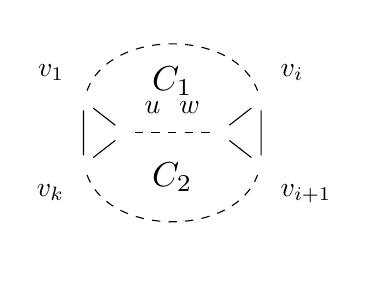
\begin{tikzpicture}[scale=1.2]
    \node (p0)[label=above left:${v_1}$] at (160:1.0cm) {};
    \node (pn) [label=above right:${v_i}$] at (20:1.0cm) {};
    \node (q0) [label=below left:${v_k}$] at (200:1.0cm) {};
    \node (qn) [label=below right:${v_{i+1}}$] at (340:1.0cm) {};
  \node (t0) [label=above right:$u$] at (180:0.5cm) {};
  \node (t1) [label=above left:$w$] at (0:0.5cm) {};
    \node (null) [draw=none, fill=none] at (270:1.25cm) {};
  
  \node (C1) [scale=1.25] [draw=none, fill=none] at (90:0.55cm) {$C_1$};
  \node (C2) [scale=1.25] [draw=none, fill=none] at (270:0.47cm) {$C_2$};
  
  \draw (p0) edge [bend left=70] (pn) [dashed];
  \draw (q0) edge [bend right=70] (qn) [dashed];
  \draw (p0) edge (q0);
  \draw (pn) edge (qn);
  \draw (p0) edge (t0);
  \draw (q0) edge (t0);
  \draw (pn) edge (t1);
  \draw (qn) edge (t1);
  \draw (t0) edge (t1) [dashed];
\end{tikzpicture}
$\qquad$
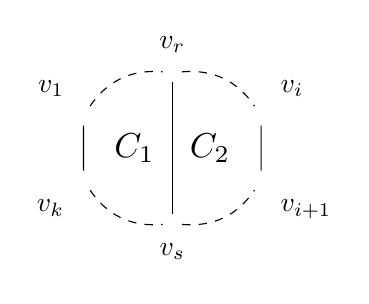
\begin{tikzpicture}[scale=1.2]
    \node (p0) [label=above left:${v_1}$] at (160:1.0cm) {};
    \node (p1) [label=above:${v_r}$] at (90:0.8cm) {};
    \node (pn) [label=above right:${v_i}$] at (20:1.0cm) {};
    \node (q0) [label=below left:${v_k}$] at (200:1.0cm) {};
    \node (q1) [label=below:${v_s}$] at (270:0.8cm) {};
    \node (qn) [label=below right:${v_{i+1}}$] at (340:1.0cm) {};
    \node (null) [draw=none, fill=none] at (270:1.25cm) {};
  
    \node (C1) [scale=1.25] [draw=none, fill=none] at (180:0.4cm) {$C_1$};
    \node (C2) [scale=1.25] [draw=none, fill=none] at (0:0.4cm) {$C_2$};
  
  \draw (p0) edge [bend left] (p1) [dashed];
  \draw (p1) edge [bend left] (pn) [dashed];
  \draw (q0) edge [bend right] (q1) [dashed];
  \draw (q1) edge [bend right] (qn) [dashed];
  \draw (p0) edge (q0);
  \draw (pn) edge (qn);
  \draw (p1) edge (q1);
\end{tikzpicture}
\caption{The proof of Lemma~\ref{L:planar3c} if $C$ is induced (left) or has
a chord (right).}
\label{poh_figure}
\end{center}
\end{figure}

Let $G$ be a triangulated plane graph. We may trivially path $2$-color the outer
triangle. Applying Lemma~\ref{L:planar3c} extends this coloring to a path
$3$-coloring of $G$.

For an arbitrary planar graph $G$ we may compute an embedding and add edges
to produce a triangulated plane graph $G'$. Any path $3$-coloring of
$G'$ will also be a path $3$-coloring of $G$. Thus Theorem~\ref{T:planar3c}
follows from Lemma~\ref{L:planar3c}.

In the construction of the path $P_3$ in Poh's proof, the
induced $u,w$-path was picked to be a $u,w$-path of shortest length.
Thus a natural way to implement Poh's algorithm is to locate $u$,
and then use a breadth-first search
to construct a $u,w$-path and/or locate
a chord edge.

\begin{algorithm}\label{A:poh_bfs}
\textbf{Input.} 
Let $C=v_1,v_2,\ldots,v_k$ be a cycle in a $2$-connected,
weakly triangulated plane
graph $G$ with adjacency list representation $\text{Adj}$.
Let 
$c$ be a length $n$ integer array representing a $2$-coloring of $C$ such
that each color class induces a path, respectively labelled
$P_1=v_1,v_2,\ldots,v_\ell$ and $P_2=v_\ell,v_{\ell+1},\ldots,v_k$. Assume that
$c[v]=0$ for each $v\in\text{Int}(C)-C$.

The concrete input to each call will be the arrays $\text{Adj}$ and $c$,
along with the ordered pair
$(v_1, v_i, v_{i+1}, v_k, v_1v_k)$ where $v_1v_k$ is represented by
a reference to $v_k$'s entry in $\text{Adj}[v_1]$. 

\textbf{Output.} For each vertex $v\in\text{Int}(C)-C$, a nonzero color will be
assigned to $c[v]$ such that $c$ represents a path $3$-coloring of
$\text{Int}(C)$ extending the original $2$-coloring of $C$. Moreover, if
$v\in \text{Int}(C)-C$ has a neighbor $u\in C$, then $c[v]\ne c[u]$.

\textbf{Procedure.} Let $u$ be the vertex immediately counter-clockwise from
$v_k$ in $\text{Adj}[v_1]$.

\textbf{Base case.} If $c[u]\ne 0$ and $u\in\{v_i,v_{i+1}\}$, then
$\text{Int}(C)=C$ is colored.

\textbf{Case 1.} Suppose that $c[u]\ne 0$ and $u\not\in\{v_i,v_{i+1}\}$.
If $c[u]=c[v_k]$, then $u\in P_2$. Make a recursive call with the input
$(v_1, v_i, v_{i+1}, u, v_1u)$. Otherwise, it must be that $c[u]=c[v_1]$
and $u\in P_1$. Iterate through $\text{Adj}[u]$ to find the entry for
$v_k$. Make a recursive call with the input $(u, v_i, v_{i+1}, v_k, uv_k)$. 

\textbf{Case 2.} Suppose that $c[u]=0$ and therefore $u\in \text{Int}(C)-C$.
Perform a breadth-first search in $\text{Int}(C)-C$, i.e. ignoring $v\in G$
if $c[v]\ne 0$, starting from the vertex $u$. Terminate the search once a vertex
$w$ is discovered that has a neighbor $v_r\in P_1$ with $c[v_r]=c[v_1]$
immediately counter-clockwise from a neighbor $v_s\in P_2$ with
$c[v_s]=c[v_k]$.

Backtrack along the search tree from $w$ to find a minimal $u,w$-path $P_3$.
For each vertex $v\in P_3$, assign $c[v]\leftarrow c_{P_3}$ where $c_{P_3}\in
\{1,2,3\}-\{c[v_1],c[v_k]\}$.

Make a recursive call with the input $(v_1, v_r, w, u, v_1u)$ to color
$\text{Int}(C_1)$, where $C_1$ is the cycle formed by the paths
$v_1,v_2,\ldots,v_r$ and $P_3$, and edges
$v_1u$, $v_rw$. Iterate through
$\text{Adj}[u]$ to find the entry for $v_k$. Make a recursive
call with input $(u, w, v_s, v_k, uv_k)$ to color $\text{Int}(C_2)$, where
$C_2$ is the cycle formed by the paths
$P_3$ and $v_k,v_{k-1},\ldots,v_s$, and edges
$v_ku$, $v_sw$.

If $v_r=v_i$ and $v_s=v_{i+1}$, then $\text{Int}(C)$ has been path $3$-colored.
Otherwise, the edge $v_rv_s$ is a chord of $C$.
Iterate through $\text{Adj}[v_r]$ to find the
entry for $v_s$, and make a recursive call with input
$(v_r, v_i, v_{i+1}, v_s, v_rv_s)$
to color the interior of the cycle $C_3=v_r,v_{r+1},\ldots,v_s$.
\end{algorithm}

\begin{figure}[ht]
\begin{center}
\SolidGraph
    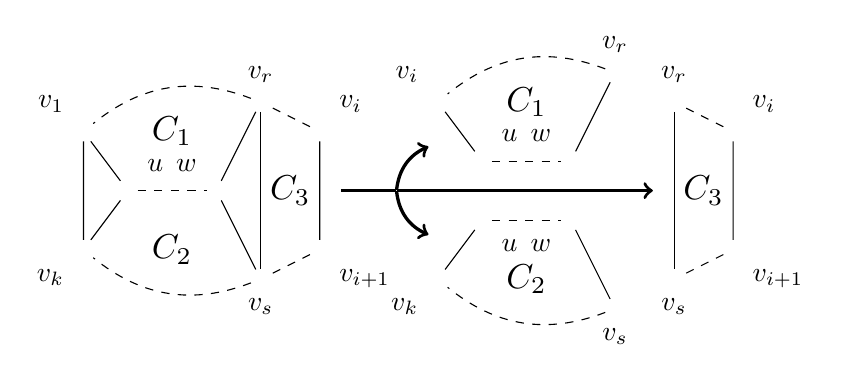
\begin{tikzpicture}[scale=0.75]
  \node (vl) [label=above right:$v_i$] at (2cm, 1cm) {};
  \node (v1) [label=above left:$v_1$] at (-2cm, 1cm) {};
  \node (vl1) [label=below right:$v_{i+1}$] at (2cm, -1cm) {};
  \node (vk) [label=below left:$v_k$] at (-2cm, -1cm) {};
  \node (w) [label=above left:$w$] at (0.25cm, 0cm) {};
  \node (u) [label=above right:$u$] at (-1.25cm, 0cm) {};
  \node (vi) [label=above:$v_r$] at (1cm, 1.5cm) {};
  \node (vj) [label=below:$v_s$] at (1cm, -1.5cm) {};
  
  \node (CP) [scale=1.25] [draw=none, fill=none] at (-0.5cm, 1cm) {$C_1$};
  \node (CQ) [scale=1.25] [draw=none, fill=none] at (-0.5cm, -1cm) {$C_2$};
  \node (Ci) [scale=1.25] [draw=none, fill=none] at (1.5cm, 0cm) {$C_3$};
  
  \node (null) [draw=none, fill=none] at (270:2.5cm) {};
  
  \draw (vl) edge (vi) [dashed];
  \draw (vi) edge [bend right] (v1) [dashed];
  \draw (vl1) edge (vj) [dashed];
  \draw (vj) edge [bend left] (vk) [dashed];
  \draw (vl) edge (vl1);
  \draw (v1) edge (vk);
  \draw (vi) edge (vj);
  \draw (v1) edge (u);
  \draw (vk) edge (u);

  \draw (u) edge (w) [dashed];
  \draw (vi) edge (w);
  \draw (vj) edge (w);

  \node (bs) [empty] at (2.35cm, 0.0cm) {};
  \node (bm) [empty] at (3.3cm, 0.0cm) {};
  \node (be1) [empty] at (3.85cm, 0.75cm) {};
  \node (be2) [empty] at (3.85cm, -0.75cm) {};
  \node (be3) [empty] at (7.65cm, 0.0cm) {};

  \draw (bs) edge [very thick] (bm);
  \draw (bm) edge[very thick, ->, bend left] (be1);
  \draw (bm) edge[very thick, ->, bend right] (be2);
  \draw (bm) edge[very thick, ->] (be3);

  \node (p0) [label=above right:$v_i$] at (9cm, 1cm) {};
  \node (q0) [label=below right:$v_{i+1}$] at (9cm, -1cm) {};
  \node (pi) [label=above:$v_r$] at (8cm, 1.5cm) {};
  \node (qj) [label=below:$v_s$] at (8cm, -1.5cm) {};
  
  \node (pi_1) [label=above:$v_r$] at (7cm, 2cm) {};
  \node (pn) [label=above left:$v_i$] at (4cm, 1.5cm) {};
  \node (t0) [label=above left:$w$] at (6.25cm, 0.5cm) {};
  \node (t1) [label=above right:$u$] at (4.75cm, 0.5cm) {};
  
  \node (CP) [scale=1.25] [draw=none, fill=none] at (5.5cm, 1.5cm) {$C_1$};
  \node (CQ) [scale=1.25] [draw=none, fill=none] at (5.5cm, -1.5cm) {$C_2$};
  \node (Ci) [scale=1.25] [draw=none, fill=none] at (8.5cm, 0cm) {$C_3$};
  
  \node (qj_1) [label=below:$v_s$] at (7cm, -2cm) {};
  \node (qn) [label=below left:$v_k$] at (4cm, -1.5cm) {};
  \node (t0_1) [label=below left:$w$] at (6.25cm, -0.5cm) {};
  \node (t1_1) [label=below right:$u$] at (4.75cm, -0.5cm) {};

  \draw (p0) edge (pi) [dashed];
  \draw (pi_1) edge [bend right] (pn) [dashed];
  \draw (q0) edge (qj) [dashed];
  \draw (qj_1) edge [bend left] (qn) [dashed];
  \draw (p0) edge (q0);
  \draw (pi) edge (qj);
  \draw (pn) edge (t1);
  \draw (qn) edge (t1_1);
  \draw (t1) edge (t0) [dashed];
  \draw (t1_1) edge (t0_1) [dashed];
  \draw (pi_1) edge (t0);
  \draw (qj_1) edge (t0_1);
\end{tikzpicture}
$\qquad$
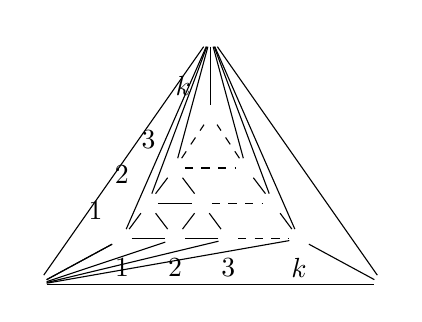
\begin{tikzpicture}[scale=0.9]
  \node (t1) at (0cm, 3.5cm) {};
  \node (t2) at (2.45cm, 0cm) {};
  \node (t3) at (-2.45cm, 0cm) {};

    \node (k1) [label=above left:$1$, label=below:$1$] at (-1.25cm, 0.65cm) {};
    \node (k2) [label=below:$2$] at (-0.5cm, 0.65cm) {};
    \node (k3) [label=below:$3$] at (0.25cm, 0.65cm) {};
    \node (kn) [label=below:$k$] at (1.25cm, 0.65cm) {};

    \node (l1) [label=above left:$2$] at (-0.88cm, 1.15cm) {};
    \node (l2) at (-0.12cm, 1.15cm) {};
    \node (ln) at (0.88cm, 1.15cm) {};

  \node (j1) [label=above left:$3$] at (-0.5cm, 1.65cm) {};
  \node (jn) at (0.5cm, 1.65cm) {};

  \node (p) [label=above left:$k$] at (0cm, 2.4cm) {};

  \begin{pgfonlayer}{bg}
	  \draw (t1) edge (t2); \draw (t3) edge (t2); \draw (t1) edge (t3);
	  \draw (k1) edge (k2); \draw (k3) edge (k2);
	  \draw (k3) edge (kn) [dashed];

	  \draw (l1) edge (l2);
	  \draw (l2) edge (ln) [dashed];

	  \draw (j1) edge (jn) [dashed];

	  \draw (j1) edge (p) [dashed];
	  \draw (jn) edge (p) [dashed];

	  \draw (t1) edge (k1); \draw (t1) edge (kn);
	  \draw (t1) edge (l1); \draw (t1) edge (ln);
	  \draw (t1) edge (p);
	  \draw (t2) edge (kn); \draw (t3) edge (k1);

	  \draw (k1) edge (l1); \draw (k2) edge (l1);
	  \draw (k2) edge (l2); \draw (k3) edge (l2);
	  \draw (kn) edge (ln);

	  \draw (l1) edge (j1); \draw (l2) edge (j1);
	  \draw (jn) edge (ln);

	  \draw (j1) edge (t1); \draw (jn) edge (t1);

	  \draw (t3) edge (k1); \draw (t3) edge (k2);
	  \draw (t3) edge (k3); \draw (t3) edge (kn);
  \end{pgfonlayer}
\end{tikzpicture}
\caption{Algorithm~\ref{A:poh_bfs}, Case~2 (left), and
the sequence of ``pyramid graphs'' $\{A_k\}_{k\in\mathbb{N}}$ on which it displays
$\Omega(n^{3/2})$ time complexity (right).}\label{F:poh_bfs}
\end{center}
\end{figure}

Unfortunately Algorithm~\ref{A:poh_bfs}
is not linear. Consider the sequence of ``pyramid graphs''
$\{A_k\}_{k\in\mathbb{N}}$ depicted in
Figure~\ref{F:poh_bfs}.
Fix $k\in\mathbb{N}$ and note that
$n=n(A_k)=k(k+1)/2+3$. Assume
that the outer triangle is path $2$-colored such that the top vertex is
assigned a color distinct from the bottom two. At depth $i$ of
Algorithm~\ref{A:poh_bfs}
the shortest path through the interior will be the path of length
$r=k-i+1$ directly along the base of the inner triangle. A breadth-first search
of this inner triangle will hit all $r(r+1)/2$ vertices in order to find this
path. Therefore the total number of operations performed will be
\[
    \Theta\left( \sum_{r=1}^k\frac{r(r+1)}{2} \right)
    =\Theta(k^3)
    =\Theta(n^{3/2}).
\]
So Poh's algorithm implemented with breadth-first search is $\Omega(n^{3/2})$.

However, the correctness of Poh's proof only relied on
locating some induced $u,w$-path.
We will show that there exists a linear time implementation of Poh's
algorithm that does not always find the shortest $u,w$-path.

For any subgraph $H$ of $G$, let $N(H)$ be the set of vertices in $V(G)$ with a
neighbor in $V(H)$. Our strategy will be to construct an induced
path $P_3=u_1,u_2,\ldots,u_d$ consisting of vertices in $N(P_1)-V(C)$.

\begin{algorithm}\label{A:poh_linear}
\textbf{Input.} Assume that $C=v_1,v_2,\ldots,v_k$ is an induced cycle of
length $4$ or more in a $2$-connected, weakly triangulated plane
graph $G$ with adjacency list representation $\text{Adj}$.
Let $u\in\text{Int}(C)-C$ be the unique vertex such that $u,v_k,v_1$ is a face.

Let $c$ be a length $n$ array of colors
representing a $2$-coloring of $C$ such
that each color class induces a path, respectively $P_1=v_1,v_2,\ldots,v_i$ and
$P_2=v_{i+1},v_{i+2},\ldots,v_k$. Let $c_{P_1}$ and $c_{P_2}$ be the colors
for $P_1$ and $P_2$, respectively. Assume $c[v]=0$ for each
$v\in\text{Int}(C)-C$.

Let $S$ be a length $n$ array of integer marks and let $m_{P_1}$ be an integer
such that for each $v\in\text{Int}(C)-C$ we have $S[v]=m_{P_1}$ if and only if
$v\in N(P_1)$.

The concrete input for each call will be the arrays $\text{Adj}$, $c$ and $S$,
along with the ordered pair $(u, uv_k)$ where $uv_k$ is represented by the
entry for $v_k$ in $\text{Adj}[u]$.

\textbf{Output.} For each vertex $v\in\text{Int}(C)-C$, a nonzero color will be
assigned to $c[v]$ such that $c$ represents a path $3$-coloring of
$\text{Int}(C)$ extending the original $2$-coloring of $C$. Moreover, if
$v\in N(P_1)-C$, then $c[v]\ne c_{P_1}$, and if $v\in N(P_2)-C$, then
$c[v]\ne c_{P_2}$.

\textbf{Outline.} As in the proof of Lemma~\ref{L:planar3c} we will
construct a $u,w$-path $P_3$
in $\text{Int}(C)-C$, but here $V(P_3)\subset N(P_1)$ and $w$
will not be known prior to constructing $P_3$.
Each vertex of $P_3$ will be colored with
$c_{P_3}\in\{1,2,3\}-\{c_{P_1},c_{P_2}\}$. Each $v\in
N(P_3)-C-P_3$ will be marked $S[v]\leftarrow m_{P_3}$.

While constructing $P_3$ we will locate each induced cycle formed by
vertices in $P_1+P_3$, and each induced cycle formed by
vertices in $P_2+P_3$. We'll make a recursive call to path $3$-color
$\text{Int}(C')$ for
each such cycle $C'$ with a non-empty interior.

\textbf{Procedure.}
Store $u_j$, the last
vertex added to $P_3=u_1,u_2,\ldots,u_j$, along with
$u_{j-1}$'s entry in $\text{Adj}[u_j]$. Define $u_0=v_k$ for the purpose
of identifying $u_{j-1}$. Track the
last edge $u_rv_s$ between $P_3$ and $P_2$ that was encountered,
represented by
$u_r\in P_3$ and the entry for $v_s\in P_2$ in $\text{Adj}[u_r]$.
Initialize $j\leftarrow 1$, $u_1\leftarrow u$, $u_rv_s\leftarrow u_1v_k$,
and color $c[u]\leftarrow c_{P_3}$. 

\textbf{Step 1.} Iterate through $\text{Adj}[u_j]$ in counter-clockwise
order, starting with
the entry counter-clockwise from $u_{j-1}$.
At each neighbor one of the following cases
will be satisfied.

While iterating through $\text{Adj}[u_j]$, keep track of an optional vertex
$y\leftarrow\text{NULL}$ that will be added to $P_3$ and become
$u_{j+1}$ once all the neighbors of $u_j$ have been handled. Store
an optional edge $u_jv_\ell\leftarrow\text{NULL}$, represented by the entry
for $v_\ell$ in $\text{Adj}[u_j]$, indicating the last neighbor of $u_j$ in
$P_1$ that was encountered. 

\textbf{Case 1.1.} Suppose that $u_jv_\ell=\text{NULL}$,
that is, no neighbor of $u_j$ in $P_1$ has been encountered yet.
See Figure~\ref{F:poh_linear_1} for a sketch of each sub-case.

\begin{figure}[ht]
\begin{center}
\SolidGraph
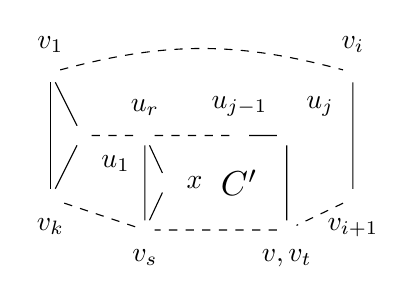
\begin{tikzpicture}[scale=1.6]
    \node (v1) [label=above:${v_1}$] at (-0.25cm, 1.0cm) {};
    \node (vi) [label=above:${v_i}$] at (2.15cm, 1.0cm) {};
    \node (vi1) [label=below:${v_{i+1}}$] at (2.15cm, 0.0cm) {};
    \node (vs) [label=below:${v_{s}}$] at (0.5cm, -0.25cm) {};
    \node (vt) [label=below:${v,v_{t}}$] at (1.625cm, -0.25cm) {};
    \node (vk) [label=below:${v_k}$] at (-0.25cm, 0.0cm) {};
    \node (u1) [label=below right:${u_1}$] at (0.0cm, 0.5cm) {};
    \node (ur) [label=above:${u_r}$] at (0.5cm, 0.5cm) {};
    \node (uj1) [label=above:${u_{j-1}}$] at (1.25cm, 0.5cm) {};
    \node (uj) [label=above right:${u_j}$] at (1.625cm, 0.5cm) {};
    \node (x) [label=right:${x}$] at (0.675cm, 0.125cm) {};

    \node (C) [scale=1.25] [draw=none, fill=none] at (1.25cm, 0.125cm) {$C'$};

    \begin{pgfonlayer}{bg}
        \draw (v1) edge[dashed, bend left=15] (vi);
        \draw (vi) edge (vi1);
        \draw (vi1) edge [dashed] (vt);
        \draw (vt) edge [dashed] (vs);
        \draw (vs) edge [dashed] (vk);
        \draw (vk) edge (v1);
        \draw (v1) edge (u1);
        \draw (vs) edge (ur);
        \draw (vk) edge (u1);
        \draw (u1) edge[dashed] (ur);
        \draw (ur) edge[dashed] (uj1);
        \draw (uj1) edge (uj);
        \draw (uj) edge (vt);
        \draw (ur) edge (x);
        \draw (vs) edge (x);
    \end{pgfonlayer}
\end{tikzpicture}
$\quad$
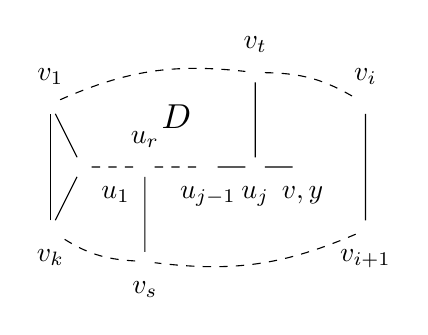
\begin{tikzpicture}[scale=1.6]
    \node (v1) [label=above:${v_1}$] at (0.0cm, 1.0cm) {};
    \node (vp) [label=above:${v_t}$] at (1.625cm, 1.25cm) {};
    \node (vi) [label=above:${v_i}$] at (2.5cm, 1.0cm) {};
    \node (vi1) [label=below:${v_{i+1}}$] at (2.5cm, 0.0cm) {};
    \node (vs) [label=below:${v_{s}}$] at (0.75cm, -0.25cm) {};
    \node (vk) [label=below:${v_k}$] at (0.0cm, 0.0cm) {};
    \node (u1) [label=below right:${u_1}$] at (0.25cm, 0.5cm) {};
    \node (ur) [label=above:${u_r}$] at (0.75cm, 0.5cm) {};
    \node (uj1) [label=below:${u_{j-1}}$] at (1.25cm, 0.5cm) {};
    \node (uj) [label=below:${u_j}$] at (1.625cm, 0.5cm) {};
    \node (y) [label=below:${v,y}$] at (2.0cm, 0.5cm) {};

    \node (D) [scale=1.25] [draw=none, fill=none] at (1.0cm, 0.9cm) {$D$};

    \begin{pgfonlayer}{bg}
        \draw (v1) edge[dashed, bend left=15] (vp);
        \draw (vp) edge[dashed, bend left=15] (vi);
        \draw (vi) edge (vi1);
        \draw (vi1) edge[dashed, bend left=15] (vs);
        \draw (vs) edge[dashed, bend left=15] (vk);
        \draw (vk) edge (v1);
        \draw (v1) edge (u1);
        \draw (vs) edge (ur);
        \draw (vk) edge (u1);
        \draw (u1) edge[dashed] (ur);
        \draw (ur) edge[dashed] (uj1);
        \draw (uj1) edge (uj);
        \draw (uj) edge (y);
        \draw (uj) edge (vp);
    \end{pgfonlayer}
\end{tikzpicture}
$\quad$
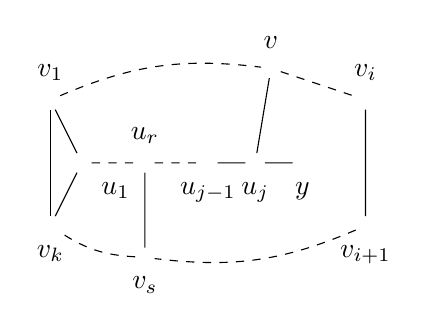
\begin{tikzpicture}[scale=1.6]
    \node (v1) [label=above:${v_1}$] at (0.0cm, 1.0cm) {};
    \node (vi) [label=above:${v_i}$] at (2.5cm, 1.0cm) {};
    \node (vi1) [label=below:${v_{i+1}}$] at (2.5cm, 0.0cm) {};
    \node (vs) [label=below:${v_{s}}$] at (0.75cm, -0.25cm) {};
    \node (vk) [label=below:${v_k}$] at (0.0cm, 0.0cm) {};
    \node (u1) [label=below right:${u_1}$] at (0.25cm, 0.5cm) {};
    \node (ur) [label=above:${u_r}$] at (0.75cm, 0.5cm) {};
    \node (uj1) [label=below:${u_{j-1}}$] at (1.25cm, 0.5cm) {};
    \node (uj) [label=below:${u_j}$] at (1.625cm, 0.5cm) {};
    \node (y) [label=below:${y}$] at (2.0cm, 0.5cm) {};
    \node (v) [label=above:${v}$] at (1.75cm, 1.25cm) {};

    \begin{pgfonlayer}{bg}
        \draw (v1) edge[dashed, bend left=15] (v);

        \draw (v) edge[dashed] (vi);
        \draw (vi) edge (vi1);
        \draw (vi1) edge[dashed, bend left=15] (vs);
        \draw (vs) edge[dashed, bend left=15] (vk);
        \draw (vk) edge (v1);
        \draw (v1) edge (u1);
        \draw (vs) edge (ur);
        \draw (vk) edge (u1);
        \draw (u1) edge[dashed] (ur);
        \draw (ur) edge[dashed] (uj1);
        \draw (uj1) edge (uj);
        \draw (uj) edge (y);
        \draw (uj) edge (v);
    \end{pgfonlayer}
\end{tikzpicture}
\caption{Algorithm~\ref{A:poh_linear}, Case~1.1.2 (left), Case~1.1.3 (middle),
and Case~1.1.4 (right).}\label{F:poh_linear_1}
\end{center}
\end{figure}

\textbf{Case 1.1.1.} Suppose $c[v]=0$ and $S[v]\ne m_{P_1}$, that is,
$v\in\text{Int}(C)-C-N(P_1)$. Assign $S[v]\leftarrow m_{P_3}$.

\textbf{Case 1.1.2.} Suppose that $c[v]=c_{P_2}$, that is, $v=v_t\in P_2$.
Observe that $P_1'=u_r,u_{r+1},\ldots, u_j$ and $P_2'=v_s,v_{s+1},\ldots,v_t$
are colored paths that, together with the edges $u_rv_s$ and $u_jv_t$,
form an induced cycle $C'$. Each uncolored vertex in
$N(P_3)\cap V(\text{Int}(C'))$ has already been marked with $m_{P_3}$.
Let
$x$ be the neighbor of $u_r$ immediately counter-clockwise from $v_s$.
If $c[x]=0$, make a recursive call with input $(x, xv_s)$
to path $3$-color $\text{Int}(C')$. Assign
$u_rv_s\leftarrow u_jv_t$ to track $u_jv_t$ as the most recent edge between
$P_3$ and $P_2$.

\textbf{Case 1.1.3.} Suppose that $c[v]=0$ and $S[v]=m_{P_1}$, that is,
$v\in N(P_1)-C$. If $y\ne\text{NULL}$, assign $S[v]\leftarrow m_{P_3}$.
Otherwise, assign $y\leftarrow v$ and color
$c[y]\leftarrow c_{P_3}$. We claim that $u_1,u_2,\ldots,u_j,y$ is an induced
path. Since $u_j\in N(P_1)$, there exists an edge $u_jv_t$ where $v_t\in P_1$.
Observe that $D=v_k,v_1,v_2,\ldots,v_t,u_j,u_{j-1},\ldots,u_1$ is a cycle in
$\text{Int}(C)$ and $y\not\in\text{Int}(D)$. Thus if an edge $yu_e$ exists with
$u_e\in P_3-u_j$,
then $y$'s entry in $\text{Adj}[u_e]$ is between $u_{e-1}$ and
$u_{e+1}$ counter-clockwise.
But $y$ would have been encountered before $u_{e+1}$
when iterating through $\text{Adj}[u_e]$, a contradiction since
$S[y]=m_{P_1}$.

\textbf{Case 1.1.4.} Suppose that $c[v]=c_{P_1}$, that is, $v\in P_1$.
Assign $u_jv_\ell\leftarrow u_jv$. If $y=\text{NULL}$, it must be
that $v=v_i\in P_1$ is the last vertex of $P_1$ and therefore $u_j=w$.
To see this, note
that the neighbor $v'$ of $u_j$ immediately clockwise from $v$ is adjacent
to $v\in P_1$, but $v'$ was not assigned to $y$. Therefore $c[v']=c_{P_2}$ and
it must be that $v'=v_{i+1}$ and $v=v_i$. Since $u_j,v_i,v_{i+1}$ is a face,
$u_j=w$ by definition.

\textbf{Case 1.2.} Suppose that $u_jv_\ell\ne\text{NULL}$. Let $z$ be
the neighbor of $u_j$ immediately counter-clockwise from $v_\ell$.
See Figure~\ref{F:poh_linear_2} for a sketch of each sub-case.

\begin{figure}[ht]
\begin{center}
\SolidGraph
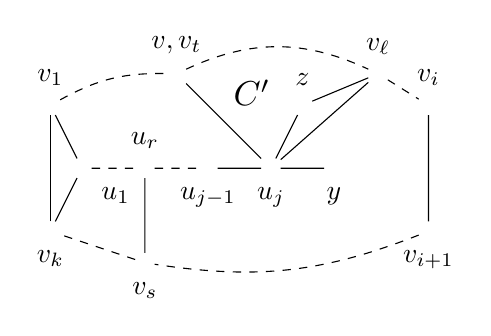
\begin{tikzpicture}[scale=1.6]
    \node (v1) [label=above:${v_1}$] at (0.0cm, 1.0cm) {};
    \node (vi) [label=above:${v_i}$] at (3.0cm, 1.0cm) {};
    \node (vi1) [label=below:${v_{i+1}}$] at (3.0cm, 0.0cm) {};
    \node (vs) [label=below:${v_{s}}$] at (0.75cm, -0.25cm) {};
    \node (vt) [label=above:${v,v_{t}}$] at (1.0cm, 1.25cm) {};
    \node (vl) [label=above:${v_{\ell}}$] at (2.6cm, 1.25cm) {};
    \node (vk) [label=below:${v_k}$] at (0.0cm, 0.0cm) {};
    \node (u1) [label=below right:${u_1}$] at (0.25cm, 0.5cm) {};
    \node (ur) [label=above:${u_r}$] at (0.75cm, 0.5cm) {};
    \node (uj1) [label=below:${u_{j-1}}$] at (1.25cm, 0.5cm) {};
    \node (uj) [label=below:${u_j}$] at (1.75cm, 0.5cm) {};
    \node (y) [label=below:${y}$] at (2.25cm, 0.5cm) {};
    \node (z) [label=above:${z}$] at (2.0cm, 1.0cm) {};

    \node (C) [scale=1.25] [draw=none, fill=none] at (1.6cm, 1.1cm) {$C'$};

    \begin{pgfonlayer}{bg}
        \draw (v1) edge[dashed, bend left=15] (vt);
        \draw (vt) edge[dashed, bend left=25] (vl);
        \draw (vl) edge[dashed] (vi);
        \draw (vi) edge (vi1);
        \draw (vi1) edge [dashed, bend left=15] (vs);
        \draw (vs) edge [dashed] (vk);
        \draw (vk) edge (v1);
        \draw (v1) edge (u1);
        \draw (vs) edge (ur);
        \draw (vk) edge (u1);
        \draw (u1) edge[dashed] (ur);
        \draw (ur) edge[dashed] (uj1);
        \draw (uj1) edge (uj);
        \draw (uj) edge (vt);
        \draw (uj) edge (vl);
        \draw (uj) edge (y);
        \draw (uj) edge (z);
        \draw (vl) edge (z);
    \end{pgfonlayer}
\end{tikzpicture}
$\qquad$
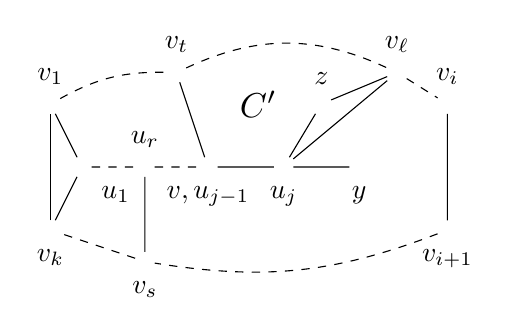
\begin{tikzpicture}[scale=1.6]
    \node (v1) [label=above:${v_1}$] at (0.0cm, 1.0cm) {};
    \node (vi) [label=above:${v_i}$] at (3.15cm, 1.0cm) {};
    \node (vi1) [label=below:${v_{i+1}}$] at (3.15cm, 0.0cm) {};
    \node (vs) [label=below:${v_{s}}$] at (0.75cm, -0.25cm) {};
    \node (vt) [label=above:${v_{t}}$] at (1.0cm, 1.25cm) {};
    \node (vl) [label=above:${v_{\ell}}$] at (2.75cm, 1.25cm) {};
    \node (vk) [label=below:${v_k}$] at (0.0cm, 0.0cm) {};
    \node (u1) [label=below right:${u_1}$] at (0.25cm, 0.5cm) {};
    \node (ur) [label=above:${u_r}$] at (0.75cm, 0.5cm) {};
    \node (uj1) [label=below:${v,u_{j-1}}$] at (1.25cm, 0.5cm) {};
    \node (uj) [label=below:${u_j}$] at (1.85cm, 0.5cm) {};
    \node (y) [label=below:${y}$] at (2.45cm, 0.5cm) {};
    \node (z) [label=above:${z}$] at (2.15cm, 1.0cm) {};

    \node (C) [scale=1.25] [draw=none, fill=none] at (1.65cm, 1.0cm) {$C'$};

    \begin{pgfonlayer}{bg}
        \draw (v1) edge[dashed, bend left=15] (vt);
        \draw (vt) edge[dashed, bend left=25] (vl);
        \draw (vl) edge[dashed] (vi);
        \draw (vi) edge (vi1);
        \draw (vi1) edge [dashed, bend left=15] (vs);
        \draw (vs) edge [dashed] (vk);
        \draw (vk) edge (v1);
        \draw (v1) edge (u1);
        \draw (vs) edge (ur);
        \draw (vk) edge (u1);
        \draw (u1) edge[dashed] (ur);
        \draw (ur) edge[dashed] (uj1);
        \draw (uj1) edge (uj);
        \draw (uj1) edge (vt);
        \draw (uj) edge (vl);
        \draw (uj) edge (y);
        \draw (uj) edge (z);
        \draw (vl) edge (z);
    \end{pgfonlayer}
\end{tikzpicture}
\caption{Algorithm~\ref{A:poh_linear}, Case~1.2.2 (left)
and Case~1.2.3 (right).}\label{F:poh_linear_2}
\end{center}
\end{figure}

\textbf{Case 1.2.1.} Suppose that $c[v]=0$, that is, $v\in\text{Int}(C)-C-P_3$.
Assign $S[v]\leftarrow m_{P_3}$.

\textbf{Case 1.2.2.} Suppose that $c[v]=c_{P_1}$. Then
$v=v_t\in P_1$ and $C'=u_j,v_t,v_{t+1},\ldots,v_\ell$ is an
induced
cycle and each uncolored vertex in $N(P_3)\cap
V(\text{Int}(C'))$ has been marked with $m_{P_3}$.
If $c[z]=0$, make a recursive call with input $(z, zv_\ell)$
to path $3$-color $\text{Int}(C')$.
Otherwise, $z=v$ and $\text{Int}(C')=C'$.

\textbf{Case 1.2.3.} Suppose that $c[v]\ne 0$ and $c[v]\ne c_{P_1}$.
If $c[v]=c_{P_2}$, then $j=1$, $v=v_k$, $u_jv_\ell=uv_1$, and there are no
uncolored neighbors of $u_j$ between $v_\ell$ and $v$.

Suppose that $c[v]=c_{P_3}$. Let $t$ be largest such that
$v_t\in P_1$ and $u_{j-1}v_{t}$ is an edge. Observe that
$C'=u_j,u_{j-1},v_t,v_{t+1},\ldots,v_\ell$ is an induced cycle. Moreover,
each uncolored vertex in $N(P_3)\cap
V(\text{Int}(C'))$ has been marked with $m_{P_3}$.
If $c[z]=0$, make a recursive call with input $(z, zv_\ell)$ to
color $\text{Int}(C')$. Otherwise, $z=v$ and $\text{Int}(C')=C'$.

\textbf{Step 2.} If $y\ne\text{NULL}$, then 
assign $j\leftarrow j+1$, $u_j\leftarrow y$, $y\leftarrow\text{NULL}$,
$u_jv_\ell\leftarrow\text{NULL}$, and return to Step~1.
Otherwise, $u_j=w$ and $\text{Int}(C)$ has been path
$3$-colored.
\end{algorithm}

\begin{figure}
\begin{center}
\OutlineGraph
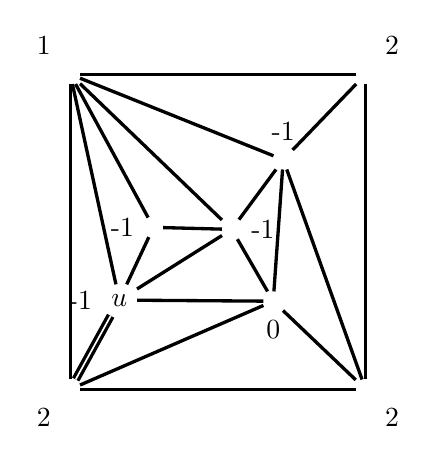
\begin{tikzpicture}
        \node (v0) [label=above left:{1}] at (-1.875000cm, 2.000000cm) {};
        \node (v1) [label=above right:{2}] at (1.875000cm, 2.000000cm) {};
        \node (v2) [label=below right:{2}] at (1.875000cm, -2.000000cm) {};
        \node (v3) [label=below left:{2}] at (-1.875000cm, -2.000000cm) {};
        \node (v4) [label=above:{-1}] at (0.829462cm, 0.915182cm) {};
        \node (v5) [label=below:{0}] at (0.702189cm, -0.881858cm) {};
        \node (v6) [label=left:{-1}] at (-1.251848cm, -0.867854cm) {$u$};
        \node (v7) [label=left:{-1}] at (-0.819321cm, 0.056225cm) {};
        \node (v8) [label=right:{-1}] at (0.175438cm, 0.030180cm) {};
        \begin{pgfonlayer}{bg}
                \draw (v5) edge [very thick] (v6);
                \draw (v6) edge [very thick] (v8);
                \draw (v6) edge [very thick] (v7);
                \draw (v7) edge [very thick] (v8);
                \draw (v5) edge [very thick] (v8);
                \draw (v4) edge [very thick] (v8);
                \draw (v4) edge [very thick] (v5);
                \draw (v0) edge [very thick] (v3);
                \draw (v0) edge [very thick] (v6);
                \draw (v0) edge [very thick] (v7);
                \draw (v0) edge [very thick] (v8);
                \draw (v0) edge [very thick] (v4);
                \draw (v0) edge [very thick] (v1);
                \draw (v1) edge [very thick] (v4);
                \draw (v1) edge [very thick] (v2);
                \draw (v2) edge [very thick] (v4);
                \draw (v2) edge [very thick] (v5);
                \draw (v2) edge [very thick] (v3);
                \draw (v3) edge [very thick] (v5);
                \draw (v3) edge [double, very thick] (v6);
        \end{pgfonlayer}
\end{tikzpicture}
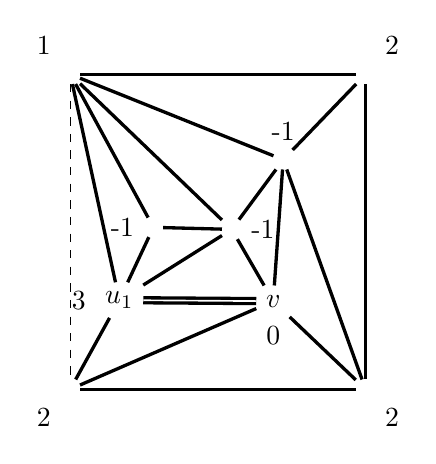
\begin{tikzpicture}
        \node (v0) [label=above left:{1}] at (-1.875000cm, 2.000000cm) {};
        \node (v1) [label=above right:{2}] at (1.875000cm, 2.000000cm) {};
        \node (v2) [label=below right:{2}] at (1.875000cm, -2.000000cm) {};
        \node (v3) [label=below left:{2}] at (-1.875000cm, -2.000000cm) {};
        \node (v4) [label=above:{-1}] at (0.829462cm, 0.915182cm) {};
        \node (v5) [label=below:{0}] at (0.702189cm, -0.881858cm) {$v$};
        \node (v6) [label=left:{3}] at (-1.251848cm, -0.867854cm) {$u_1$};
        \node (v7) [label=left:{-1}] at (-0.819321cm, 0.056225cm) {};
        \node (v8) [label=right:{-1}] at (0.175438cm, 0.030180cm) {};
        \begin{pgfonlayer}{bg}
                \draw (v5) edge [double, very thick] (v6);
                \draw (v6) edge [very thick] (v8);
                \draw (v6) edge [very thick] (v7);
                \draw (v7) edge [very thick] (v8);
                \draw (v5) edge [very thick] (v8);
                \draw (v4) edge [very thick] (v8);
                \draw (v4) edge [very thick] (v5);
                \draw (v0) edge [dashed] (v3);
                \draw (v0) edge [very thick] (v6);
                \draw (v0) edge [very thick] (v7);
                \draw (v0) edge [very thick] (v8);
                \draw (v0) edge [very thick] (v4);
                \draw (v0) edge [very thick] (v1);
                \draw (v1) edge [very thick] (v4);
                \draw (v1) edge [very thick] (v2);
                \draw (v2) edge [very thick] (v4);
                \draw (v2) edge [very thick] (v5);
                \draw (v2) edge [very thick] (v3);
                \draw (v3) edge [very thick] (v5);
                \draw (v3) edge [very thick] (v6);
        \end{pgfonlayer}
\end{tikzpicture}
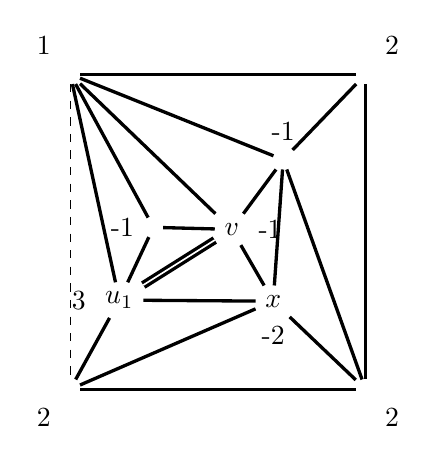
\begin{tikzpicture}
        \node (v0) [label=above left:{1}] at (-1.875000cm, 2.000000cm) {
};
        \node (v1) [label=above right:{2}] at (1.875000cm, 2.000000cm) {};
        \node (v2) [label=below right:{2}] at (1.875000cm, -2.000000cm) {};
        \node (v3) [label=below left:{2}] at (-1.875000cm, -2.000000cm) {};
        \node (v4) [label=above:{-1}] at (0.829462cm, 0.915182cm) {};
        \node (v5) [label=below:{-2}] at (0.702189cm, -0.881858cm) {$x$};
        \node (v6) [label=left:{3}] at (-1.251848cm, -0.867854cm) {$u_1$};
        \node (v7) [label=left:{-1}] at (-0.819321cm, 0.056225cm) {};
        \node (v8) [label=right:{-1}] at (0.175438cm, 0.030180cm) {$v$};
        \begin{pgfonlayer}{bg}
                \draw (v6) edge [double, very thick] (v8);
                \draw (v6) edge [very thick] (v7);
                \draw (v7) edge [very thick] (v8);
                \draw (v5) edge [very thick] (v8);
                \draw (v5) edge [very thick] (v6);
                \draw (v4) edge [very thick] (v8);
                \draw (v4) edge [very thick] (v5);
                \draw (v0) edge [dashed] (v3);
                \draw (v0) edge [very thick] (v6);
                \draw (v0) edge [very thick] (v7);
                \draw (v0) edge [very thick] (v8);
                \draw (v0) edge [very thick] (v4);
                \draw (v0) edge [very thick] (v1);
                \draw (v1) edge [very thick] (v4);
                \draw (v1) edge [very thick] (v2);
                \draw (v2) edge [very thick] (v4);
                \draw (v2) edge [very thick] (v5);
                \draw (v2) edge [very thick] (v3);
                \draw (v3) edge [very thick] (v5);
                \draw (v3) edge [very thick] (v6);
        \end{pgfonlayer}
\end{tikzpicture}

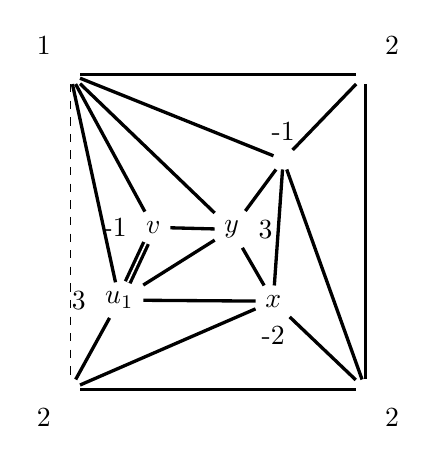
\begin{tikzpicture}
        \node (v0) [label=above left:{1}] at (-1.875000cm, 2.000000cm) {
};
        \node (v1) [label=above right:{2}] at (1.875000cm, 2.000000cm) {};
        \node (v2) [label=below right:{2}] at (1.875000cm, -2.000000cm) {};
        \node (v3) [label=below left:{2}] at (-1.875000cm, -2.000000cm) {};
        \node (v4) [label=above:{-1}] at (0.829462cm, 0.915182cm) {};
        \node (v5) [label=below:{-2}] at (0.702189cm, -0.881858cm) {$x$};
        \node (v6) [label=left:{3}] at (-1.251848cm, -0.867854cm) {$u_1$};
        \node (v7) [label=left:{-1}] at (-0.819321cm, 0.056225cm) {$v$};
        \node (v8) [label=right:{3}] at (0.175438cm, 0.030180cm) {$y$};
        \begin{pgfonlayer}{bg}
                \draw (v0) edge [very thick] (v6);
                \draw (v5) edge [very thick] (v8);
                \draw (v5) edge [very thick] (v6);
                \draw (v4) edge [very thick] (v8);
                \draw (v4) edge [very thick] (v5);
                \draw (v7) edge [very thick] (v8);
                \draw (v0) edge [very thick] (v7);
                \draw (v0) edge [very thick] (v8);
                \draw (v0) edge [very thick] (v4);
                \draw (v0) edge [very thick] (v1);
                \draw (v1) edge [very thick] (v4);
                \draw (v1) edge [very thick] (v2);
                \draw (v2) edge [very thick] (v4);
                \draw (v2) edge [very thick] (v5);
                \draw (v2) edge [very thick] (v3);
                \draw (v3) edge [very thick] (v5);
                \draw (v3) edge [very thick] (v6);
                \draw (v6) edge [very thick] (v8);
                \draw (v6) edge [double, very thick] (v7);
                \draw (v0) edge [dashed] (v3);
        \end{pgfonlayer}
\end{tikzpicture}
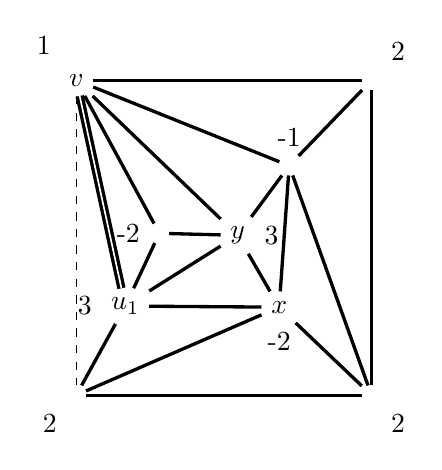
\begin{tikzpicture}
        \node (v0) [label=above left:{1}] at (-1.875000cm, 2.000000cm) {$v$};
        \node (v1) [label=above right:{2}] at (1.875000cm, 2.000000cm) {};
        \node (v2) [label=below right:{2}] at (1.875000cm, -2.000000cm) {};
        \node (v3) [label=below left:{2}] at (-1.875000cm, -2.000000cm) {};
        \node (v4) [label=above:{-1}] at (0.829462cm, 0.915182cm) {};
        \node (v5) [label=below:{-2}] at (0.702189cm, -0.881858cm) {$x$};
        \node (v6) [label=left:{3}] at (-1.251848cm, -0.867854cm) {$u_1$};
        \node (v7) [label=left:{-2}] at (-0.819321cm, 0.056225cm) {};
        \node (v8) [label=right:{3}] at (0.175438cm, 0.030180cm) {$y$};
        \begin{pgfonlayer}{bg}
                \draw (v0) edge [double, very thick] (v6);
                \draw (v5) edge [very thick] (v8);
                \draw (v5) edge [very thick] (v6);
                \draw (v4) edge [very thick] (v8);
                \draw (v4) edge [very thick] (v5);
                \draw (v7) edge [very thick] (v8);
                \draw (v0) edge [very thick] (v7);
                \draw (v0) edge [very thick] (v8);
                \draw (v0) edge [very thick] (v4);
                \draw (v0) edge [very thick] (v1);
                \draw (v1) edge [very thick] (v4);
                \draw (v1) edge [very thick] (v2);
                \draw (v2) edge [very thick] (v4);
                \draw (v2) edge [very thick] (v5);
                \draw (v2) edge [very thick] (v3);
                \draw (v3) edge [very thick] (v5);
                \draw (v3) edge [very thick] (v6);
                \draw (v6) edge [very thick] (v8);
                \draw (v6) edge [very thick] (v7);
                \draw (v0) edge [dashed] (v3);
        \end{pgfonlayer}
\end{tikzpicture}
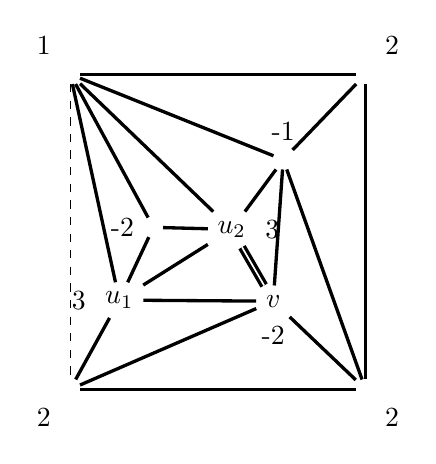
\begin{tikzpicture}
        \node (v0) [label=above left:{1}] at (-1.875000cm, 2.000000cm) {};
        \node (v1) [label=above right:{2}] at (1.875000cm, 2.000000cm) {};
        \node (v2) [label=below right:{2}] at (1.875000cm, -2.000000cm) {};
        \node (v3) [label=below left:{2}] at (-1.875000cm, -2.000000cm) {};
        \node (v4) [label=above:{-1}] at (0.829462cm, 0.915182cm) {};
        \node (v5) [label=below:{-2}] at (0.702189cm, -0.881858cm) {$v$};
        \node (v6) [label=left:{3}] at (-1.251848cm, -0.867854cm) {$u_1$};
        \node (v7) [label=left:{-2}] at (-0.819321cm, 0.056225cm) {};
        \node (v8) [label=right:{3}] at (0.175438cm, 0.030180cm) {$u_2$};
        \begin{pgfonlayer}{bg}
                \draw (v5) edge [double, very thick] (v8);
                \draw (v4) edge [very thick] (v8);
                \draw (v4) edge [very thick] (v5);
                \draw (v7) edge [very thick] (v8);
                \draw (v5) edge [very thick] (v6);
                \draw (v0) edge [very thick] (v6);
                \draw (v0) edge [very thick] (v7);
                \draw (v0) edge [very thick] (v8);
                \draw (v0) edge [very thick] (v4);
                \draw (v0) edge [very thick] (v1);
                \draw (v1) edge [very thick] (v4);
                \draw (v1) edge [very thick] (v2);
                \draw (v2) edge [very thick] (v4);
                \draw (v2) edge [very thick] (v5);
                \draw (v2) edge [very thick] (v3);
                \draw (v3) edge [very thick] (v5);
                \draw (v3) edge [very thick] (v6);
                \draw (v6) edge [very thick] (v8);
                \draw (v6) edge [very thick] (v7);
                \draw (v0) edge [dashed] (v3);
        \end{pgfonlayer}
\end{tikzpicture}

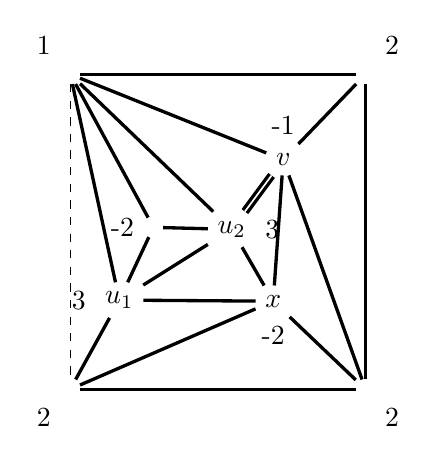
\begin{tikzpicture}
        \node (v0) [label=above left:{1}] at (-1.875000cm, 2.000000cm) {};
        \node (v1) [label=above right:{2}] at (1.875000cm, 2.000000cm) {};
        \node (v2) [label=below right:{2}] at (1.875000cm, -2.000000cm) {};
        \node (v3) [label=below left:{2}] at (-1.875000cm, -2.000000cm) {};
        \node (v4) [label=above:{-1}] at (0.829462cm, 0.915182cm) {$v$};
        \node (v5) [label=below:{-2}] at (0.702189cm, -0.881858cm) {$x$};
        \node (v6) [label=left:{3}] at (-1.251848cm, -0.867854cm) {$u_1$};
        \node (v7) [label=left:{-2}] at (-0.819321cm, 0.056225cm) {};
        \node (v8) [label=right:{3}] at (0.175438cm, 0.030180cm) {$u_2$};
        \begin{pgfonlayer}{bg}
                \draw (v4) edge [double, very thick] (v8);
                \draw (v7) edge [very thick] (v8);
                \draw (v5) edge [very thick] (v8);
                \draw (v5) edge [very thick] (v6);
                \draw (v4) edge [very thick] (v5);
                \draw (v0) edge [very thick] (v6);
                \draw (v0) edge [very thick] (v7);
                \draw (v0) edge [very thick] (v8);
                \draw (v0) edge [very thick] (v4);
                \draw (v0) edge [very thick] (v1);
                \draw (v1) edge [very thick] (v4);
                \draw (v1) edge [very thick] (v2);
                \draw (v2) edge [very thick] (v4);
                \draw (v2) edge [very thick] (v5);
                \draw (v2) edge [very thick] (v3);
                \draw (v3) edge [very thick] (v5);
                \draw (v3) edge [very thick] (v6);
                \draw (v6) edge [very thick] (v8);
                \draw (v6) edge [very thick] (v7);
                \draw (v0) edge [dashed] (v3);
        \end{pgfonlayer}
\end{tikzpicture}
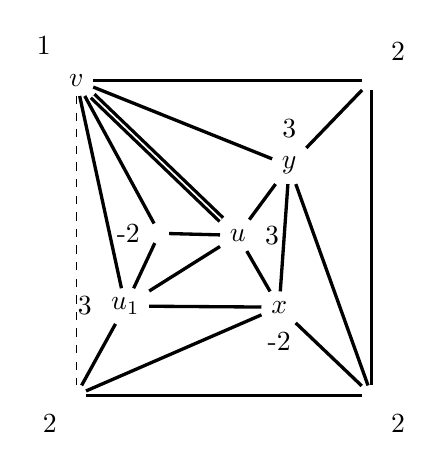
\begin{tikzpicture}
        \node (v0) [label=above left:{1}] at (-1.875000cm, 2.000000cm) {$v$};
        \node (v1) [label=above right:{2}] at (1.875000cm, 2.000000cm) {};
        \node (v2) [label=below right:{2}] at (1.875000cm, -2.000000cm) {};
        \node (v3) [label=below left:{2}] at (-1.875000cm, -2.000000cm) {};
        \node (v4) [label=above:{3}] at (0.829462cm, 0.915182cm) {$y$};
        \node (v5) [label=below:{-2}] at (0.702189cm, -0.881858cm) {$x$};
        \node (v6) [label=left:{3}] at (-1.251848cm, -0.867854cm) {$u_1$};
        \node (v7) [label=left:{-2}] at (-0.819321cm, 0.056225cm) {};
        \node (v8) [label=right:{3}] at (0.175438cm, 0.030180cm) {$u$};
        \begin{pgfonlayer}{bg}
                \draw (v7) edge [very thick] (v8);
                \draw (v5) edge [very thick] (v8);
                \draw (v5) edge [very thick] (v6);
                \draw (v4) edge [very thick] (v8);
                \draw (v4) edge [very thick] (v5);
                \draw (v0) edge [very thick] (v6);
                \draw (v0) edge [very thick] (v7);
                \draw (v0) edge [double, very thick] (v8);
                \draw (v0) edge [very thick] (v4);
                \draw (v0) edge [very thick] (v1);
                \draw (v1) edge [very thick] (v4);
                \draw (v1) edge [very thick] (v2);
                \draw (v2) edge [very thick] (v4);
                \draw (v2) edge [very thick] (v5);
                \draw (v2) edge [very thick] (v3);
                \draw (v3) edge [very thick] (v5);
                \draw (v3) edge [very thick] (v6);
                \draw (v6) edge [very thick] (v8);
                \draw (v6) edge [very thick] (v7);
                \draw (v0) edge [dashed] (v3);
        \end{pgfonlayer}
\end{tikzpicture}
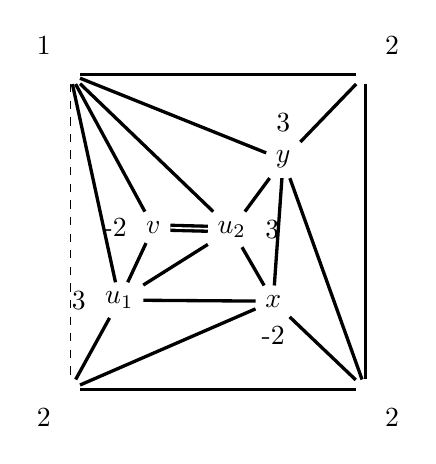
\begin{tikzpicture}
        \node (v0) [label=above left:{1}] at (-1.875000cm, 2.000000cm) {
};
        \node (v1) [label=above right:{2}] at (1.875000cm, 2.000000cm) {};
        \node (v2) [label=below right:{2}] at (1.875000cm, -2.000000cm) {};
        \node (v3) [label=below left:{2}] at (-1.875000cm, -2.000000cm) {};
        \node (v4) [label=above:{3}] at (0.829462cm, 0.915182cm) {$y$};
        \node (v5) [label=below:{-2}] at (0.702189cm, -0.881858cm) {$x$};
        \node (v6) [label=left:{3}] at (-1.251848cm, -0.867854cm) {$u_1$};
        \node (v7) [label=left:{-2}] at (-0.819321cm, 0.056225cm) {$v$};
        \node (v8) [label=right:{3}] at (0.175438cm, 0.030180cm) {$u_2$};
        \begin{pgfonlayer}{bg}
                \draw (v6) edge [very thick] (v8);
                \draw (v5) edge [very thick] (v8);
                \draw (v5) edge [very thick] (v6);
                \draw (v4) edge [very thick] (v8);
                \draw (v4) edge [very thick] (v5);
                \draw (v0) edge [very thick] (v8);
                \draw (v0) edge [very thick] (v4);
                \draw (v0) edge [very thick] (v1);
                \draw (v1) edge [very thick] (v4);
                \draw (v1) edge [very thick] (v2);
                \draw (v2) edge [very thick] (v4);
                \draw (v2) edge [very thick] (v5);
                \draw (v2) edge [very thick] (v3);
                \draw (v3) edge [very thick] (v5);
                \draw (v3) edge [very thick] (v6);
                \draw (v0) edge [dashed] (v3);
                \draw (v0) edge [very thick](v6);
                \draw (v0) edge [very thick](v7);
                \draw (v6) edge [very thick](v7);
                \draw (v7) edge [double, very thick] (v8);
        \end{pgfonlayer}
\end{tikzpicture}

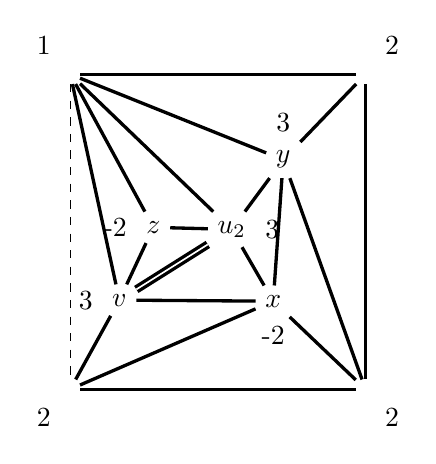
\begin{tikzpicture}
        \node (v0) [label=above left:{1}] at (-1.875000cm, 2.000000cm) {};
        \node (v1) [label=above right:{2}] at (1.875000cm, 2.000000cm) {};
        \node (v2) [label=below right:{2}] at (1.875000cm, -2.000000cm) {};
        \node (v3) [label=below left:{2}] at (-1.875000cm, -2.000000cm) {};
        \node (v4) [label=above:{3}] at (0.829462cm, 0.915182cm) {$y$};
        \node (v5) [label=below:{-2}] at (0.702189cm, -0.881858cm) {$x$};
        \node (v6) [label=left:{3}] at (-1.251848cm, -0.867854cm) {$v$};
        \node (v7) [label=left:{-2}] at (-0.819321cm, 0.056225cm) {$z$};
        \node (v8) [label=right:{3}] at (0.175438cm, 0.030180cm) {$u_2$};
        \begin{pgfonlayer}{bg}
                \draw (v6) edge [double, very thick] (v8);
                \draw (v5) edge [very thick] (v8);
                \draw (v5) edge [very thick] (v6);
                \draw (v4) edge [very thick] (v8);
                \draw (v4) edge [very thick] (v5);
                \draw (v0) edge [very thick] (v8);
                \draw (v0) edge [very thick] (v4);
                \draw (v0) edge [very thick] (v1);
                \draw (v1) edge [very thick] (v4);
                \draw (v1) edge [very thick] (v2);
                \draw (v2) edge [very thick] (v4);
                \draw (v2) edge [very thick] (v5);
                \draw (v2) edge [very thick] (v3);
                \draw (v3) edge [very thick] (v5);
                \draw (v3) edge [very thick] (v6);
                \draw (v0) edge [dashed] (v3);
                \draw (v0) [very thick] edge (v6);
                \draw (v0) [very thick] edge (v7);
                \draw (v6) [very thick] edge (v7);
                \draw (v7) [very thick] edge (v8);
        \end{pgfonlayer}
\end{tikzpicture}
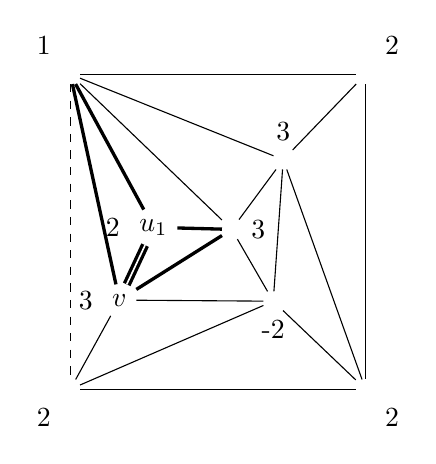
\begin{tikzpicture}
        \node (v0) [label=above left:{1}] at (-1.875000cm, 2.000000cm) {};
        \node (v1) [label=above right:{2}] at (1.875000cm, 2.000000cm) {};
        \node (v2) [label=below right:{2}] at (1.875000cm, -2.000000cm) {};
        \node (v3) [label=below left:{2}] at (-1.875000cm, -2.000000cm) {};
        \node (v4) [label=above:{3}] at (0.829462cm, 0.915182cm) {};
        \node (v5) [label=below:{-2}] at (0.702189cm, -0.881858cm) {};
        \node (v6) [label=left:{3}] at (-1.251848cm, -0.867854cm) {$v$};
        \node (v7) [label=left:{2}] at (-0.819321cm, 0.056225cm) {$u_1$};
        \node (v8) [label=right:{3}] at (0.175438cm, 0.030180cm) {};
        \begin{pgfonlayer}{bg}
                \draw (v0) edge [very thick] (v7);
                \draw (v7) edge [very thick] (v8);
                \draw (v0) edge [very thick] (v6);
                \draw (v0) edge [thin] (v8);
                \draw (v6) edge [very thick] (v8);
                \draw (v6) edge [double, very thick] (v7);
                \draw (v5) edge [thin] (v8);
                \draw (v5) edge [thin] (v6);
                \draw (v4) edge [thin] (v8);
                \draw (v4) edge [thin] (v5);
                \draw (v0) edge [thin] (v4);
                \draw (v0) edge [thin] (v1);
                \draw (v1) edge [thin] (v4);
                \draw (v1) edge [thin] (v2);
                \draw (v2) edge [thin] (v4);
                \draw (v2) edge [thin] (v5);
                \draw (v2) edge [thin] (v3);
                \draw (v3) edge [thin] (v5);
                \draw (v3) edge [thin] (v6);
                \draw (v0) edge [dashed] (v3);
        \end{pgfonlayer}
\end{tikzpicture}
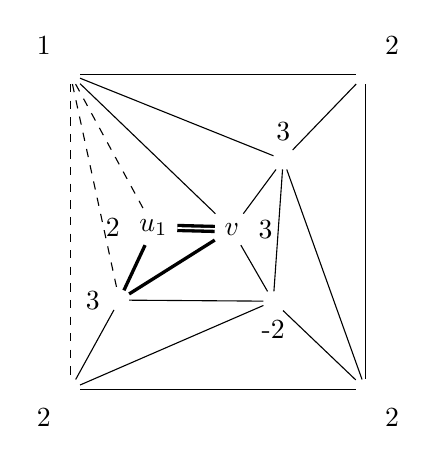
\begin{tikzpicture}
        \node (v0) [label=above left:{1}] at (-1.875000cm, 2.000000cm) {};
        \node (v1) [label=above right:{2}] at (1.875000cm, 2.000000cm) {};
        \node (v2) [label=below right:{2}] at (1.875000cm, -2.000000cm) {};
        \node (v3) [label=below left:{2}] at (-1.875000cm, -2.000000cm) {};
        \node (v4) [label=above:{3}] at (0.829462cm, 0.915182cm) {};
        \node (v5) [label=below:{-2}] at (0.702189cm, -0.881858cm) {};
        \node (v6) [label=left:{3}] at (-1.251848cm, -0.867854cm) {};
        \node (v7) [label=left:{2}] at (-0.819321cm, 0.056225cm) {$u_1$};
        \node (v8) [label=right:{3}] at (0.175438cm, 0.030180cm) {$v$};
        \begin{pgfonlayer}{bg}
                \draw (v7) edge [double, very thick] (v8);
                \draw (v5) edge [thin] (v8);
                \draw (v5) edge [thin] (v6);
                \draw (v4) edge [thin] (v8);
                \draw (v4) edge [thin] (v5);
                \draw (v0) edge [thin] (v8);
                \draw (v0) edge [thin] (v4);
                \draw (v0) edge [thin] (v1);
                \draw (v1) edge [thin] (v4);
                \draw (v1) edge [thin] (v2);
                \draw (v2) edge [thin] (v4);
                \draw (v2) edge [thin] (v5);
                \draw (v2) edge [thin] (v3);
                \draw (v3) edge [thin] (v5);
                \draw (v3) edge [thin] (v6);
                \draw (v6) edge [very thick] (v8);
                \draw (v0) edge [dashed] (v3);
                \draw (v0) edge [dashed] (v6);
                \draw (v0) edge [dashed] (v7);
                \draw (v6) edge [very thick] (v7);
        \end{pgfonlayer}
\end{tikzpicture}
\caption{An example of Algorithm~\ref{A:poh_linear}. Each vertex $v\in G$ is
labelled with $c[v]$ if $c[v]>0$, and labelled with $-S[v]$ otherwise.}
\label{F:poh_example}
\end{center}
\end{figure}

\begin{figure}
\begin{center}
\OutlineGraph
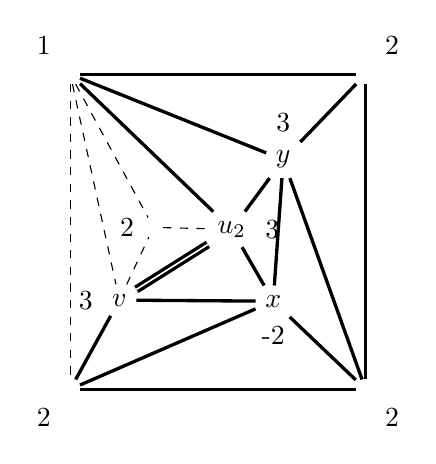
\begin{tikzpicture}
        \node (v0) [label=above left:{1}] at (-1.875000cm, 2.000000cm) {};
        \node (v1) [label=above right:{2}] at (1.875000cm, 2.000000cm) {};
        \node (v2) [label=below right:{2}] at (1.875000cm, -2.000000cm) {};
        \node (v3) [label=below left:{2}] at (-1.875000cm, -2.000000cm) {};
        \node (v4) [label=above:{3}] at (0.829462cm, 0.915182cm) {$y$};
        \node (v5) [label=below:{-2}] at (0.702189cm, -0.881858cm) {$x$};
        \node (v6) [label=left:{3}] at (-1.251848cm, -0.867854cm) {$v$};
        \node (v7) [label=left:{2}] at (-0.819321cm, 0.056225cm) {};
        \node (v8) [label=right:{3}] at (0.175438cm, 0.030180cm) {$u_2$};
        \begin{pgfonlayer}{bg}
                \draw (v6) edge [double, very thick] (v8);
                \draw (v5) edge [very thick] (v8);
                \draw (v5) edge [very thick] (v6);
                \draw (v4) edge [very thick] (v8);
                \draw (v4) edge [very thick] (v5);
                \draw (v0) edge [very thick] (v8);
                \draw (v0) edge [very thick] (v4);
                \draw (v0) edge [very thick] (v1);
                \draw (v1) edge [very thick] (v4);
                \draw (v1) edge [very thick] (v2);
                \draw (v2) edge [very thick] (v4);
                \draw (v2) edge [very thick] (v5);
                \draw (v2) edge [very thick] (v3);
                \draw (v3) edge [very thick] (v5);
                \draw (v3) edge [very thick] (v6);
                \draw (v0) edge [dashed] (v3);
                \draw (v0) edge [dashed] (v6);
                \draw (v0) edge [dashed] (v7);
                \draw (v6) edge [dashed] (v7);
                \draw (v7) edge [dashed] (v8);
        \end{pgfonlayer}
\end{tikzpicture}
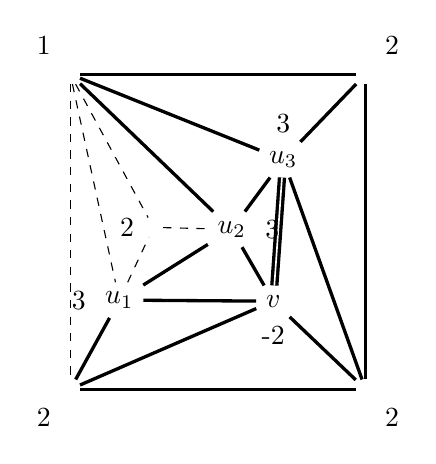
\begin{tikzpicture}
        \node (v0) [label=above left:{1}] at (-1.875000cm, 2.000000cm) {};
        \node (v1) [label=above right:{2}] at (1.875000cm, 2.000000cm) {};
        \node (v2) [label=below right:{2}] at (1.875000cm, -2.000000cm) {};
        \node (v3) [label=below left:{2}] at (-1.875000cm, -2.000000cm) {};
        \node (v4) [label=above:{3}] at (0.829462cm, 0.915182cm) {$u_3$};
        \node (v5) [label=below:{-2}] at (0.702189cm, -0.881858cm) {$v$};
        \node (v6) [label=left:{3}] at (-1.251848cm, -0.867854cm) {$u_1$};
        \node (v7) [label=left:{2}] at (-0.819321cm, 0.056225cm) {};
        \node (v8) [label=right:{3}] at (0.175438cm, 0.030180cm) {$u_2$};
        \begin{pgfonlayer}{bg}
                \draw (v4) edge [double, very thick] (v5);
                \draw (v4) edge [very thick] (v8);
                \draw (v5) edge [very thick] (v8);
                \draw (v5) edge [very thick] (v6);
                \draw (v0) edge [very thick] (v8);
                \draw (v0) edge [very thick] (v4);
                \draw (v0) edge [very thick] (v1);
                \draw (v1) edge [very thick] (v4);
                \draw (v1) edge [very thick] (v2);
                \draw (v2) edge [very thick] (v4);
                \draw (v2) edge [very thick] (v5);
                \draw (v2) edge [very thick] (v3);
                \draw (v3) edge [very thick] (v5);
                \draw (v3) edge [very thick] (v6);
                \draw (v6) edge [very thick] (v8);
                \draw (v0) edge [dashed] (v3);
                \draw (v0) edge [dashed] (v6);
                \draw (v0) edge [dashed] (v7);
                \draw (v6) edge [dashed] (v7);
                \draw (v7) edge [dashed] (v8);
        \end{pgfonlayer}
\end{tikzpicture}
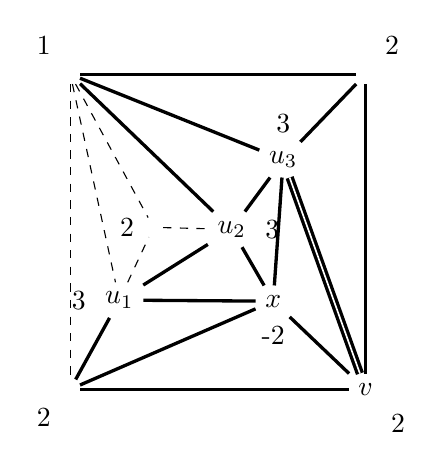
\begin{tikzpicture}
        \node (v0) [label=above left:{1}] at (-1.875000cm, 2.000000cm) {};
        \node (v1) [label=above right:{2}] at (1.875000cm, 2.000000cm) {};
        \node (v2) [label=below right:{2}] at (1.875000cm, -2.000000cm) {$v$};
        \node (v3) [label=below left:{2}] at (-1.875000cm, -2.000000cm) {};
        \node (v4) [label=above:{3}] at (0.829462cm, 0.915182cm) {$u_3$};
        \node (v5) [label=below:{-2}] at (0.702189cm, -0.881858cm) {$x$};
        \node (v6) [label=left:{3}] at (-1.251848cm, -0.867854cm) {$u_1$};
        \node (v7) [label=left:{2}] at (-0.819321cm, 0.056225cm) {};
        \node (v8) [label=right:{3}] at (0.175438cm, 0.030180cm) {$u_2$};
        \begin{pgfonlayer}{bg}
                \draw (v4) edge [very thick] (v5);
                \draw (v4) edge [very thick] (v8);
                \draw (v5) edge [very thick] (v8);
                \draw (v5) edge [very thick] (v6);
                \draw (v0) edge [very thick] (v8);
                \draw (v0) edge [very thick] (v4);
                \draw (v0) edge [very thick] (v1);
                \draw (v1) edge [very thick] (v4);
                \draw (v1) edge [very thick] (v2);
                \draw (v2) edge [double, very thick] (v4);
                \draw (v2) edge [very thick] (v5);
                \draw (v2) edge [very thick] (v3);
                \draw (v3) edge [very thick] (v5);
                \draw (v3) edge [very thick] (v6);
                \draw (v6) edge [very thick] (v8);
                \draw (v0) edge [dashed] (v3);
                \draw (v0) edge [dashed] (v6);
                \draw (v0) edge [dashed] (v7);
                \draw (v6) edge [dashed] (v7);
                \draw (v7) edge [dashed] (v8);
        \end{pgfonlayer}
\end{tikzpicture}

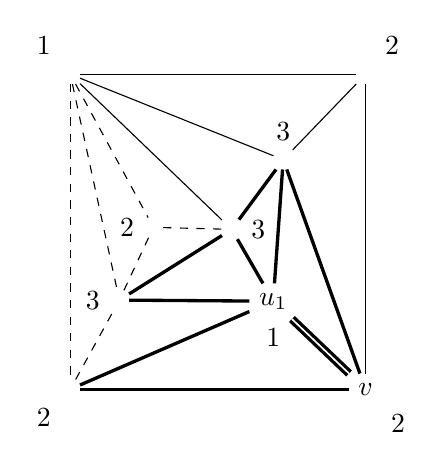
\begin{tikzpicture}
        \node (v0) [label=above left:{1}] at (-1.875000cm, 2.000000cm) {};
        \node (v1) [label=above right:{2}] at (1.875000cm, 2.000000cm) {};
        \node (v2) [label=below right:{2}] at (1.875000cm, -2.000000cm) {$v$};
        \node (v3) [label=below left:{2}] at (-1.875000cm, -2.000000cm) {};
        \node (v4) [label=above:{3}] at (0.829462cm, 0.915182cm) {};
        \node (v5) [label=below:{1}] at (0.702189cm, -0.881858cm) {$u_1$};
        \node (v6) [label=left:{3}] at (-1.251848cm, -0.867854cm) {};
        \node (v7) [label=left:{2}] at (-0.819321cm, 0.056225cm) {};
        \node (v8) [label=right:{3}] at (0.175438cm, 0.030180cm) {};
        \begin{pgfonlayer}{bg}
                \draw (v3) edge [very thick] (v5);
                \draw (v5) edge [very thick] (v8);
                \draw (v5) edge [very thick] (v6);
                \draw (v2) edge [very thick] (v4);
                \draw (v2) edge [double, very thick] (v5);
                \draw (v2) edge [very thick] (v3);
                \draw (v3) edge [dashed] (v6);
                \draw (v4) edge [very thick] (v8);
                \draw (v4) edge [very thick] (v5);
                \draw (v6) edge [very thick] (v8);
                \draw (v0) edge [thin] (v8);
                \draw (v0) edge [thin] (v4);
                \draw (v0) edge [thin] (v1);
                \draw (v1) edge [thin] (v4);
                \draw (v1) edge [thin] (v2);
                \draw (v0) edge [dashed] (v3);
                \draw (v0) edge [dashed] (v6);
                \draw (v0) edge [dashed] (v7);
                \draw (v6) edge [dashed] (v7);
                \draw (v7) edge [dashed] (v8);
        \end{pgfonlayer}
\end{tikzpicture}
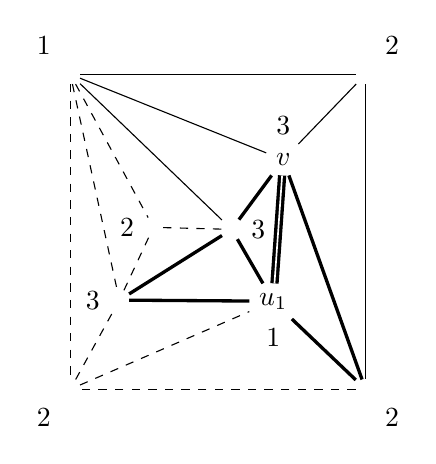
\begin{tikzpicture}
        \node (v0) [label=above left:{1}] at (-1.875000cm, 2.000000cm) {};
        \node (v1) [label=above right:{2}] at (1.875000cm, 2.000000cm) {};
        \node (v2) [label=below right:{2}] at (1.875000cm, -2.000000cm) {};
        \node (v3) [label=below left:{2}] at (-1.875000cm, -2.000000cm) {};
        \node (v4) [label=above:{3}] at (0.829462cm, 0.915182cm) {$v$};
        \node (v5) [label=below:{1}] at (0.702189cm, -0.881858cm) {$u_1$};
        \node (v6) [label=left:{3}] at (-1.251848cm, -0.867854cm) {};
        \node (v7) [label=left:{2}] at (-0.819321cm, 0.056225cm) {};
        \node (v8) [label=right:{3}] at (0.175438cm, 0.030180cm) {};
        \begin{pgfonlayer}{bg}
                \draw (v3) edge [dashed] (v5);
                \draw (v5) edge [very thick] (v8);
                \draw (v5) edge [very thick] (v6);
                \draw (v2) edge [very thick] (v4);
                \draw (v2) edge [very thick] (v5);
                \draw (v2) edge [dashed] (v3);
                \draw (v3) edge [dashed] (v6);
                \draw (v4) edge [very thick] (v8);
                \draw (v4) edge [double, very thick] (v5);
                \draw (v6) edge [very thick] (v8);
                \draw (v0) edge [thin] (v8);
                \draw (v0) edge [thin] (v4);
                \draw (v0) edge [thin] (v1);
                \draw (v1) edge [thin] (v4);
                \draw (v1) edge [thin] (v2);
                \draw (v0) edge [dashed] (v3);
                \draw (v0) edge [dashed] (v6);
                \draw (v0) edge [dashed] (v7);
                \draw (v6) edge [dashed] (v7);
                \draw (v7) edge [dashed] (v8);
        \end{pgfonlayer}
\end{tikzpicture}
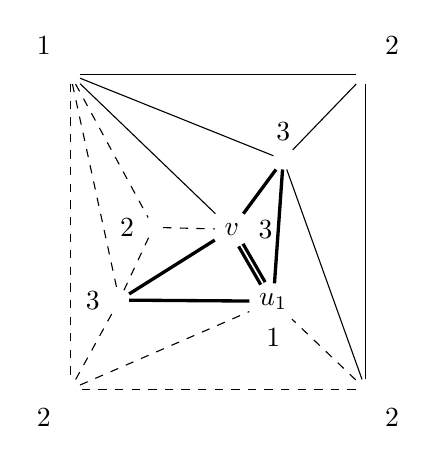
\begin{tikzpicture}
        \node (v0) [label=above left:{1}] at (-1.875000cm, 2.000000cm) {};
        \node (v1) [label=above right:{2}] at (1.875000cm, 2.000000cm) {};
        \node (v2) [label=below right:{2}] at (1.875000cm, -2.000000cm) {};
        \node (v3) [label=below left:{2}] at (-1.875000cm, -2.000000cm) {};
        \node (v4) [label=above:{3}] at (0.829462cm, 0.915182cm) {};
        \node (v5) [label=below:{1}] at (0.702189cm, -0.881858cm) {$u_1$};
        \node (v6) [label=left:{3}] at (-1.251848cm, -0.867854cm) {};
        \node (v7) [label=left:{2}] at (-0.819321cm, 0.056225cm) {};
        \node (v8) [label=right:{3}] at (0.175438cm, 0.030180cm) {$v$};
        \begin{pgfonlayer}{bg}
                \draw (v3) edge [dashed] (v5);
                \draw (v5) edge [double, very thick] (v8);
                \draw (v5) edge [very thick] (v6);
                \draw (v2) edge [thin] (v4);
                \draw (v2) edge [dashed] (v5);
                \draw (v2) edge [dashed] (v3);
                \draw (v3) edge [dashed] (v6);
                \draw (v4) edge [very thick] (v8);
                \draw (v4) edge [very thick] (v5);
                \draw (v6) edge [very thick] (v8);
                \draw (v0) edge [thin] (v8);
                \draw (v0) edge [thin] (v4);
                \draw (v0) edge [thin] (v1);
                \draw (v1) edge [thin] (v4);
                \draw (v1) edge [thin] (v2);
                \draw (v0) edge [dashed] (v3);
                \draw (v0) edge [dashed] (v6);
                \draw (v0) edge [dashed] (v7);
                \draw (v6) edge [dashed] (v7);
                \draw (v7) edge [dashed] (v8);
        \end{pgfonlayer}
\end{tikzpicture}

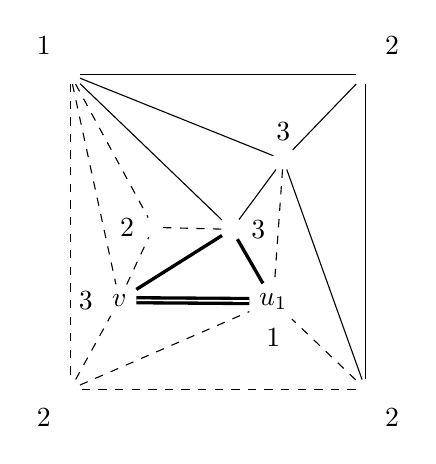
\begin{tikzpicture}
        \node (v0) [label=above left:{1}] at (-1.875000cm, 2.000000cm) {};
        \node (v1) [label=above right:{2}] at (1.875000cm, 2.000000cm) {};
        \node (v2) [label=below right:{2}] at (1.875000cm, -2.000000cm) {};
        \node (v3) [label=below left:{2}] at (-1.875000cm, -2.000000cm) {};
        \node (v4) [label=above:{3}] at (0.829462cm, 0.915182cm) {};
        \node (v5) [label=below:{1}] at (0.702189cm, -0.881858cm) {$u_1$};
        \node (v6) [label=left:{3}] at (-1.251848cm, -0.867854cm) {$v$};
        \node (v7) [label=left:{2}] at (-0.819321cm, 0.056225cm) {};
        \node (v8) [label=right:{3}] at (0.175438cm, 0.030180cm) {};
        \begin{pgfonlayer}{bg}
                \draw (v5) edge [double, very thick] (v6);
                \draw (v4) edge [thin] (v8);
                \draw (v0) edge [thin] (v8);
                \draw (v0) edge [thin] (v4);
                \draw (v0) edge [thin] (v1);
                \draw (v1) edge [thin] (v4);
                \draw (v1) edge [thin] (v2);
                \draw (v0) edge [dashed] (v3);
                \draw (v0) edge [dashed] (v6);
                \draw (v0) edge [dashed] (v7);
                \draw (v2) [thin] edge (v4);
                \draw (v2) edge [dashed] (v5);
                \draw (v2) edge [dashed] (v3);
                \draw (v3) edge [dashed] (v5);
                \draw (v3) edge [dashed] (v6);
                \draw (v4) edge [dashed] (v5);
                \draw (v5) edge [very thick] (v8);
                \draw (v6) edge [very thick] (v8);
                \draw (v6) edge [dashed] (v7);
                \draw (v7) edge [dashed] (v8);
        \end{pgfonlayer}
\end{tikzpicture}
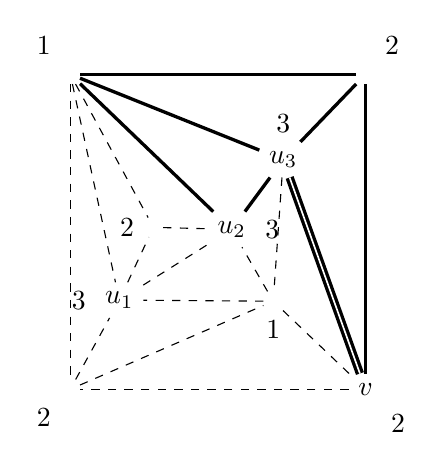
\begin{tikzpicture}
        \node (v0) [label=above left:{1}] at (-1.875000cm, 2.000000cm) {};
        \node (v1) [label=above right:{2}] at (1.875000cm, 2.000000cm) {};
        \node (v2) [label=below right:{2}] at (1.875000cm, -2.000000cm) {$v$};
        \node (v3) [label=below left:{2}] at (-1.875000cm, -2.000000cm) {};
        \node (v4) [label=above:{3}] at (0.829462cm, 0.915182cm) {$u_3$};
        \node (v5) [label=below:{1}] at (0.702189cm, -0.881858cm) {};
        \node (v6) [label=left:{3}] at (-1.251848cm, -0.867854cm) {$u_1$};
        \node (v7) [label=left:{2}] at (-0.819321cm, 0.056225cm) {};
        \node (v8) [label=right:{3}] at (0.175438cm, 0.030180cm) {$u_2$};
        \begin{pgfonlayer}{bg}
                \draw (v2) edge [double, very thick] (v4);
                \draw (v4) edge [very thick] (v8);
                \draw (v0) edge [very thick] (v8);
                \draw (v0) edge [very thick] (v4);
                \draw (v0) edge [very thick] (v1);
                \draw (v1) edge [very thick] (v4);
                \draw (v1) edge [very thick] (v2);
                \draw (v0) edge [dashed] (v3);
                \draw (v0) edge [dashed] (v6);
                \draw (v0) edge [dashed] (v7);
                \draw (v2) edge [dashed] (v5);
                \draw (v2) edge [dashed] (v3);
                \draw (v3) edge [dashed] (v5);
                \draw (v3) edge [dashed] (v6);
                \draw (v4) edge [dashed] (v5);
                \draw (v5) edge [dashed] (v8);
                \draw (v5) edge [dashed] (v6);
                \draw (v6) edge [dashed] (v8);
                \draw (v6) edge [dashed] (v7);
                \draw (v7) edge [dashed] (v8);
        \end{pgfonlayer}
\end{tikzpicture}
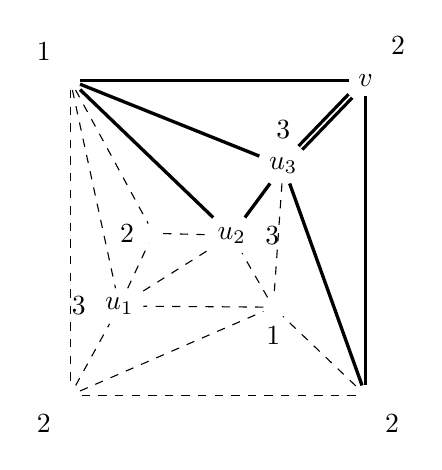
\begin{tikzpicture}
        \node (v0) [label=above left:{1}] at (-1.875000cm, 2.000000cm) {};
        \node (v1) [label=above right:{2}] at (1.875000cm, 2.000000cm) {$v$};
        \node (v2) [label=below right:{2}] at (1.875000cm, -2.000000cm) {};
        \node (v3) [label=below left:{2}] at (-1.875000cm, -2.000000cm) {};
        \node (v4) [label=above:{3}] at (0.829462cm, 0.915182cm) {$u_3$};
        \node (v5) [label=below:{1}] at (0.702189cm, -0.881858cm) {};
        \node (v6) [label=left:{3}] at (-1.251848cm, -0.867854cm) {$u_1$};
        \node (v7) [label=left:{2}] at (-0.819321cm, 0.056225cm) {};
        \node (v8) [label=right:{3}] at (0.175438cm, 0.030180cm) {$u_2$};
        \begin{pgfonlayer}{bg}
                \draw (v2) edge [very thick] (v4);
                \draw (v4) edge [very thick] (v8);
                \draw (v0) edge [very thick] (v8);
                \draw (v0) edge [very thick] (v4);
                \draw (v0) edge [very thick] (v1);
                \draw (v1) edge [double, very thick] (v4);
                \draw (v1) edge [very thick] (v2);
                \draw (v0) edge [dashed] (v3);
                \draw (v0) edge [dashed] (v6);
                \draw (v0) edge [dashed] (v7);
                \draw (v2) edge [dashed] (v5);
                \draw (v2) edge [dashed] (v3);
                \draw (v3) edge [dashed] (v5);
                \draw (v3) edge [dashed] (v6);
                \draw (v4) edge [dashed] (v5);
                \draw (v5) edge [dashed] (v8);
                \draw (v5) edge [dashed] (v6);
                \draw (v6) edge [dashed] (v8);
                \draw (v6) edge [dashed] (v7);
                \draw (v7) edge [dashed] (v8);
        \end{pgfonlayer}
\end{tikzpicture}

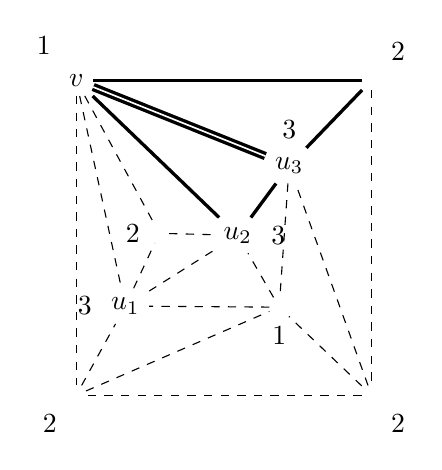
\begin{tikzpicture}
        \node (v0) [label=above left:{1}] at (-1.875000cm, 2.000000cm) {$v$};
        \node (v1) [label=above right:{2}] at (1.875000cm, 2.000000cm) {};
        \node (v2) [label=below right:{2}] at (1.875000cm, -2.000000cm) {};
        \node (v3) [label=below left:{2}] at (-1.875000cm, -2.000000cm) {};
        \node (v4) [label=above:{3}] at (0.829462cm, 0.915182cm) {$u_3$};
        \node (v5) [label=below:{1}] at (0.702189cm, -0.881858cm) {};
        \node (v6) [label=left:{3}] at (-1.251848cm, -0.867854cm) {$u_1$};
        \node (v7) [label=left:{2}] at (-0.819321cm, 0.056225cm) {};
        \node (v8) [label=right:{3}] at (0.175438cm, 0.030180cm) {$u_2$};
        \begin{pgfonlayer}{bg}
                \draw (v2) edge [dashed] (v4);
                \draw (v4) edge [very thick] (v8);
                \draw (v0) edge [very thick] (v8);
                \draw (v0) edge [double, very thick] (v4);
                \draw (v0) edge [very thick] (v1);
                \draw (v1) edge [very thick] (v4);
                \draw (v1) edge [dashed] (v2);
                \draw (v0) edge [dashed] (v3);
                \draw (v0) edge [dashed] (v6);
                \draw (v0) edge [dashed] (v7);
                \draw (v2) edge [dashed] (v5);
                \draw (v2) edge [dashed] (v3);
                \draw (v3) edge [dashed] (v5);
                \draw (v3) edge [dashed] (v6);
                \draw (v4) edge [dashed] (v5);
                \draw (v5) edge [dashed] (v8);
                \draw (v5) edge [dashed] (v6);
                \draw (v6) edge [dashed] (v8);
                \draw (v6) edge [dashed] (v7);
                \draw (v7) edge [dashed] (v8);
        \end{pgfonlayer}
\end{tikzpicture}
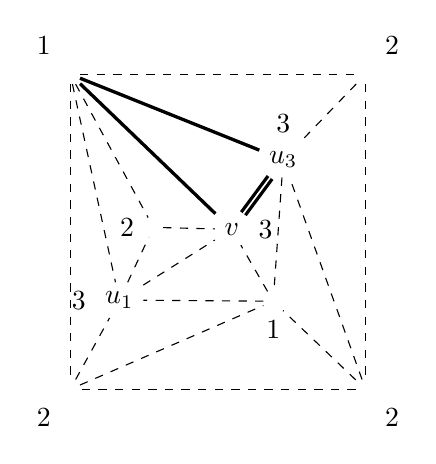
\begin{tikzpicture}
        \node (v0) [label=above left:{1}] at (-1.875000cm, 2.000000cm) {};
        \node (v1) [label=above right:{2}] at (1.875000cm, 2.000000cm) {};
        \node (v2) [label=below right:{2}] at (1.875000cm, -2.000000cm) {};
        \node (v3) [label=below left:{2}] at (-1.875000cm, -2.000000cm) {};
        \node (v4) [label=above:{3}] at (0.829462cm, 0.915182cm) {$u_3$};
        \node (v5) [label=below:{1}] at (0.702189cm, -0.881858cm) {};
        \node (v6) [label=left:{3}] at (-1.251848cm, -0.867854cm) {$u_1$};
        \node (v7) [label=left:{2}] at (-0.819321cm, 0.056225cm) {};
        \node (v8) [label=right:{3}] at (0.175438cm, 0.030180cm) {$v$};
        \begin{pgfonlayer}{bg}
                \draw (v4) edge [double, very thick] (v8);
                \draw (v0) edge [dashed] (v3);
                \draw (v0) edge [dashed] (v6);
                \draw (v0) edge [dashed] (v7);
                \draw (v0) edge [very thick] (v8);
                \draw (v0) edge [very thick] (v4);
                \draw (v0) edge [dashed] (v1);
                \draw (v1) edge [dashed] (v4);
                \draw (v1) edge [dashed] (v2);
                \draw (v2) edge [dashed] (v4);
                \draw (v2) edge [dashed] (v5);
                \draw (v2) edge [dashed] (v3);
                \draw (v3) edge [dashed] (v5);
                \draw (v3) edge [dashed] (v6);
                \draw (v4) edge [dashed] (v5);
                \draw (v5) edge [dashed] (v8);
                \draw (v5) edge [dashed] (v6);
                \draw (v6) edge [dashed] (v8);
                \draw (v6) edge [dashed] (v7);
                \draw (v7) edge [dashed] (v8);
        \end{pgfonlayer}
\end{tikzpicture}
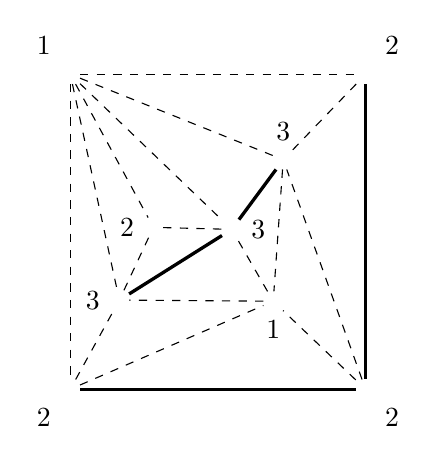
\begin{tikzpicture}
        \node (v0) [label=above left:{1}] at (-1.875000cm, 2.000000cm) {};
        \node (v1) [label=above right:{2}] at (1.875000cm, 2.000000cm) {};
        \node (v2) [label=below right:{2}] at (1.875000cm, -2.000000cm) {};
        \node (v3) [label=below left:{2}] at (-1.875000cm, -2.000000cm) {};
        \node (v4) [label=above:{3}] at (0.829462cm, 0.915182cm) {};
        \node (v5) [label=below:{1}] at (0.702189cm, -0.881858cm) {};
        \node (v6) [label=left:{3}] at (-1.251848cm, -0.867854cm) {};
        \node (v7) [label=left:{2}] at (-0.819321cm, 0.056225cm) {};
        \node (v8) [label=right:{3}] at (0.175438cm, 0.030180cm) {};
        \begin{pgfonlayer}{bg}
                \draw (v0) edge [dashed] (v1);
                \draw (v0) edge [dashed](v3);
                \draw (v0) edge [dashed](v6);
                \draw (v0) edge [dashed](v7);
                \draw (v0) edge [dashed](v8);
                \draw (v0) edge [dashed](v4);
                \draw (v1) edge [dashed](v4);
                \draw (v1) edge [very thick](v2);
                \draw (v2) edge [dashed](v4);
                \draw (v2) edge [dashed](v5);
                \draw (v2) edge [very thick](v3);
                \draw (v3) edge [dashed](v5);
                \draw (v3) edge [dashed](v6);
                \draw (v4) edge [very thick](v8);
                \draw (v4) edge [dashed](v5);
                \draw (v5) edge [dashed](v8);
                \draw (v5) edge [dashed](v6);
                \draw (v6) edge [very thick](v8);
                \draw (v6) edge [dashed](v7);
                \draw (v7) edge [dashed](v8);
        \end{pgfonlayer}
\end{tikzpicture}
\caption{An Algorithm~\ref{A:poh_linear} example, continued from
Figure~\ref{F:poh_example}.}
\label{F:poh_example_cont}
\end{center}
\end{figure}

While executing Algorithm~\ref{A:poh_linear} we iterate through
the adjacency list of each vertex $v\in G$ exactly twice: once to
orient $\text{Adj}[v]$
around a particular edge when $v$ is colored,
and once to examine each neighbor in $\text{Adj}[v]$ during Step~1.
Therefore the time complexity of the algorithm is
$\mathcal{O}(m)=\mathcal{O}(n)$. See Figure~\ref{F:poh_example} 
and Figure~\ref{F:poh_example_cont} for a concrete example of
Algorithm~\ref{A:poh_linear}.

Given a triangulated plane graph $G$ with adjacency list representation
$\text{Adj}$, we can set up the initial conditions for
Algorithm~\ref{A:poh_linear} as follows. First, create length $n$ integer
arrays for $c$ and $S$, initializing each entry to zero.
Let $C=v_1,v_2,v_3$ be the outer triangle of $G$,
labeled in clockwise order.
Color $c[v_1]\leftarrow 1$, $c[v_2]\leftarrow 2$, and
$c[v_3]\leftarrow 2$.
Iterate through $\text{Adj}[v_1]$ and mark $S[v]\leftarrow 1$ for each
neighbor $v$ of $v_1$.
Let $u$ be the vertex immediately counter-clockwise from $v_3$ in
$\text{Adj}[v_1]$. The vertex $u$ and the entry for $v_3$ in $\text{Adj}[u]$,
together with $\text{Adj}$, $c$, and $S$ form a valid input for
Algorithm~\ref{A:poh_linear}.

\section{Path List-Coloring}

In this section we describe a linear time algorithm to path color
plane graphs such that each vertex receives a color from a specified list.
Hartman showed that this is always possible when each vertex is given a
list of $3$ colors~\cite[Thm.~4.1]{Har1997}. Around the same
time \v{S}krekovski proved a
slightly weaker result using the same coloring
strategy~\cite[Thm.~2.2b]{Skr1999}.

The path list-coloring procedure discussed in this section is
based on the constructive proofs found in Hartman and
\v{S}krekovski's papers, but it ``localizes'' the logic to proceed through the
graph one edge at a time. The resulting algorithm
will produce different colorings in some situations.

A \defterm{list assignment} of a graph $G$ is
a function $L:V(G)\to P_{<\aleph_0}(\mathbb{N})$ assigning
a finite set of colors to each vertex. If $L$ is a list assignment of $G$,
an \defterm{$L$-coloring} of $G$ is a coloring function
$c:V(G)\to\mathbb{N}$ such that $c(v)\in L(v)$ for each $v\in V(G)$.

Given a graph $G$ and a coloring $c$ of $G$, for each $v\in G$ we
define $\text{deg}_c(v)$ to be the number of neighbors of $v$ that share a color
with $v$. Equivalently, $\text{deg}_c(v)$ is the degree of $v$ in the subgraph
of $G$ induced by the color class of $c(v)$.

Let $C$ be the outer face of a $2$-connected, weakly triangulated plane graph
$G$ and let $u,v\in C$ be vertices.
If $n(G)\ge3$, then $C$ is a cycle and we
define $C[u,v]$ to be the clockwise $u,v$-path
around $C$. If $n(G)<3$ then we define $C[u,v]=C$ if
$u\ne v$, and $C[u,u]=u$.

\begin{lemma}\label{L:hartman3}
Let $G$ be a $2$-connected, weakly triangulated plane graph with outer face
$C$. Let $x,y,z\in C$ be vertices (not necessarily distinct) such that
$z\in C[x,y]$. Let $L$ be a list assignment of $G$ such that
\begin{align*}
    |L(v)| &= 1 \text{ for } v\in\{x,y,z\},\\
    |L(v)| &\ge 2 \text{ for } v\in C-\{x,y,z\},\\
    |L(v)| &\ge 3 \text{ for } v\in G-C,
\end{align*}
and if $v\in C[x,z]-z$, then $L(v)\cap L(z)=\emptyset$.
There exists a path $L$-coloring of $G$ such that $\text{deg}_c(x)\le 1$,
$\text{deg}_c(y)\le 1$, and $\text{deg}_c(z)\le 1$. Moreover,
if $z=y$ or $C[z,y]=z,y$ and $L(z)\cap L(y)=\emptyset$,
then $\text{deg}_c(z)=0$.
\end{lemma}

\begin{proof}
Define $c(x)\in L(x)$, $c(y)\in L(y)$, and $c(z)\in L(z)$ to be the color in
each respective list.

Suppose that $m=|E(G)|\le 2$ and therefore $G=C$.
If $m=0$, then $n(G)=1$ and $x=y$.
If $m=1$, then $n(G)= 2$. If $x\ne y$, then $C=x,y$ and $G$ is colored.
If $x=y$, then the remaining vertex
$v\in G-C[x,y]$ satisfies $|L(v)|\ge 2$. Choose $c(v)\in L(v)-\{c(x)\}$.

We proceed by induction on $m$ the number of edges. Let
$u_1,u_2,\ldots,u_k$ label the neighbors of $z$ in counter-clockwise
order such that $u_1$ is the vertex immediately counter-clockwise from $z$ around $C$
and $u_k$ is the vertex clockwise from $z$ around $C$.

\begin{figure}[ht]
\begin{center}
\SolidGraph
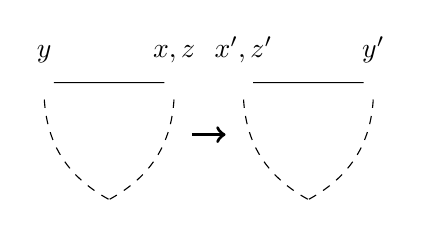
\begin{tikzpicture}[scale=1.1]
    \node (y) at (0.0cm, 1.35cm) [label=above:${y}$] {};
    \node (x) at (1.5cm, 1.35cm) [label=above:${x,z}$] {};
    \node (bot) [empty] at (0.75cm, 0.0cm) {};

    \begin{pgfonlayer}{bg}
        \draw (x) edge (y);
        \draw (bot) edge [dashed, bend right] (x);
        \draw (bot) edge [dashed, bend left] (y);
    \end{pgfonlayer}

    \node (yb) at (2.3cm, 1.35cm) [label=above:${x',z'}$] {};
    \node (xb) at (3.8cm, 1.35cm) [label=above:${y'}$] {};
    \node (botb) [empty] at (3.05cm, 0.0cm) {};

    \node (bs) [empty] at (1.7cm, 0.75cm) {};
    \node (be) [empty] at (2.1cm, 0.75cm) {};

    \draw (bs) edge[very thick, ->] (be);

    \begin{pgfonlayer}{bg}
        \draw (xb) edge (yb);
        \draw (botb) edge [dashed, bend right] (xb);
        \draw (botb) edge [dashed, bend left] (yb);
    \end{pgfonlayer}
\end{tikzpicture}
$\quad$
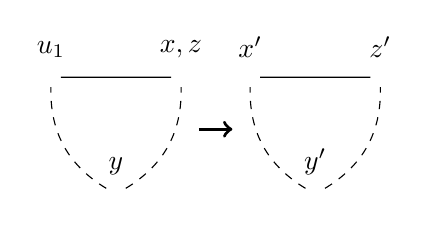
\begin{tikzpicture}[scale=1.1]
    \node (u1) at (0.0cm, 1.35cm) [label=above:${u_1}$] {};
    \node (x) at (1.5cm, 1.35cm) [label=above:${x,z}$] {};
    \node (y) [label=above:${y}$] at (0.75cm, 0.0cm) {};

    \begin{pgfonlayer}{bg}
        \draw (x) edge (u1);
        \draw (y) edge [dashed, bend right] (x);
        \draw (y) edge [dashed, bend left] (u1);
    \end{pgfonlayer}

    \node (u1b) at (2.3cm, 1.35cm) [label=above:${x'}$] {};
    \node (xb) at (3.8cm, 1.35cm) [label=above:${z'}$] {};
    \node (yb) [label=above:${y'}$] at (3.05cm, 0.0cm) {};

    \node (bs) [empty] at (1.7cm, 0.75cm) {};
    \node (be) [empty] at (2.1cm, 0.75cm) {};

    \draw (bs) edge[very thick, ->] (be);

    \begin{pgfonlayer}{bg}
        \draw (xb) edge (u1b);
        \draw (yb) edge [dashed, bend right] (xb);
        \draw (yb) edge [dashed, bend left] (u1b);
    \end{pgfonlayer}
\end{tikzpicture}
$\quad$
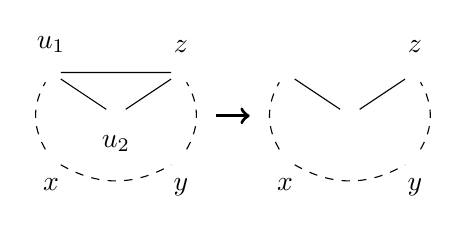
\begin{tikzpicture}[scale=1.1]
    \node (u1) at (0.0cm, 1.0cm) [label=above:${u_1}$] {};
    \node (v) at (0.75cm, 0.5cm) [label=below:${u_2}$] {};
    \node (z) at (1.5cm, 1.0cm) [label=above:${z}$] {};
    \node (x) at (0.0cm, 0.0cm) [label=below:${x}$] {};
    \node (y) at (1.5cm, 0.0cm) [label=below:${y}$] {};

    \begin{pgfonlayer}{bg}
        \draw (z) edge (u1);
        \draw (z) edge (v);
        \draw (u1) edge (v);
        \draw (y) edge [dashed, bend right] (z);
        \draw (x) edge [dashed, bend left] (u1);
        \draw (x) edge [dashed, bend right] (y);
    \end{pgfonlayer}

    \node (u1b) at (2.7cm, 1.0cm) {};
    \node (vb) at (3.45cm, 0.5cm) {};
    \node (zb) at (4.2cm, 1.0cm) [label=above:${z}$] {};
    \node (xb) at (2.7cm, 0.0cm) [label=below:${x}$] {};
    \node (yb) at (4.2cm, 0.0cm) [label=below:${y}$] {};

    \node (bs) [empty] at (1.9cm, 0.5cm) {};
    \node (be) [empty] at (2.3cm, 0.5cm) {};

    \draw (bs) edge[very thick, ->] (be);

    \begin{pgfonlayer}{bg}
        \draw (zb) edge (vb);
        \draw (u1b) edge (vb);
        \draw (yb) edge [dashed, bend right] (zb);
        \draw (xb) edge [dashed, bend left] (u1b);
        \draw (xb) edge [dashed, bend right] (yb);
    \end{pgfonlayer}
\end{tikzpicture}
    \caption{The proof of Lemma~\ref{L:hartman3}, Case~1 (left), Case~2
    (middle), and Case~3.1 (right).}
\end{center}
\end{figure}

\textbf{Case 1.}
Suppose that $u_1=y$. Note that $z=x$ since $z\in C[x,y]$. Therefore
$V(C[z,y])=V(C)$ and $|V(C[z,y])|\ge 3$.
Apply the lemma with vertices re-labeled as $x'=y$, $y'=x$,
and $z'=y$ to find a path $L$-coloring $c$ of $G$.

\textbf{Case 2.}
Suppose that $u_1\ne y$ and $z=x$. Then $u_1\in C-C[x,z]$
and $|L(u_1)|\ge 2$. Pick $c(u_1)\in L(u_1)-c(z)$. Define
$L'(u_1)=\{c(u_1)\}$ and $L'(v)=L(v)$ for each $v\in G-u_1$. Apply the
lemma to path $L'$-color $G$ with designated vertices $x'=u_1$, $y'=y$, and $z'=z$.

\textbf{Case 3.}
Suppose that $u_1\ne y$ and $z\ne x$. 
Our strategy will be to apply the inductive hypothesis to $G-zu_1$
with the embedding inherited from $G$.
Because $u_1\in C[x,z]$, it is guaranteed that $L(u_1)\cap L(z)=\emptyset$.
Thus any path $L$-coloring of $G-zu_1$ will also be a path $L$-coloring
of $G$.

\textbf{Case 3.1.}
Suppose that $u_2\in G-C$. Define $L'(u_2)=L(u_2)-c(z)$ and
$L'(v)=L(v)$ for each $v\in G-u_2$. Note that $|L'(u_2)|\ge |L(v)|-1\ge 2$.
Let $C'$ be the outer face of $G-zu_1$
and observe that $C'[x,z]$ is equal to $C[x,z]$ with the edge $u_1z$ removed
and the path $u_1,u_2,z$ added. Since $|L'(u_2)|\ge 2$ and $L'(u_2)\cap
L'(z)=\emptyset$, we may apply the inductive hypothesis
to find a path $L'$-coloring of $G-zu_1$.

\textbf{Case 3.2.}
Suppose that $u_2\in C$. Observe that $u_2$ is a cut-vertex of
$G-zu_1$.
Define $C_1=C[u_2,u_1]+u_1u_2$ and
$C_2=C[z,u_2]+zu_2$. Define $G_1=\text{Int}(C_1)$ and $G_2=\text{Int}(C_2)$.
The subgraphs $G_1$ and $G_2$ are the two $2$-connected components (blocks) of
$G-zu_1$. Note that if $k=2$, then $G_1=G-z$ and $G_2=z,u_2$.

In each subsequent case we will apply the inductive
hypothesis to produce a path $L$-coloring $c_1$ of $G_1$ and a path
$L$-coloring $c_2$ of $G_2$ such that $c_1(u_2)=c_2(u_2)$. Let
$c$ be the $L$-coloring of $G$ defined by $v\mapsto c_1(v)$ for $v\in G_1$
and $v\mapsto c_2(v)$ for $v\in G_2$.
Observe that $\text{deg}_c(v)=\text{deg}_{c_1}(v)$
for each $v\in G_1-u_2$, $\text{deg}_c(v)=\text{deg}_{c_2}(v)$ for each
$v\in G_2-u_2$, and
$\text{deg}_c(u_2)=\text{deg}_{c_1}(u_2)+\text{deg}_{c_2}(u_2)$.
To show that $c$ is a path $L$-coloring of $G$ it suffices to show that
$\text{deg}_{c}(u_2)\le 2$.

\begin{figure}[ht]
\begin{center}
\SolidGraph
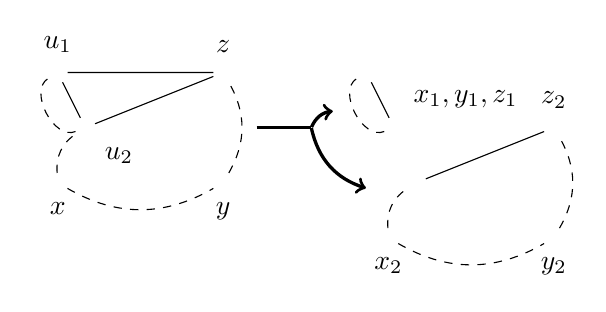
\begin{tikzpicture}[scale=1.4]
    \node (u1) at (0.0cm, 1.0cm) [label=above:${u_1}$] {};
    \node (v) at (0.25cm, 0.5cm) [label=below right:${u_2}$] {};
    \node (z) at (1.5cm, 1.0cm) [label=above:${z}$] {};
    \node (x) at (0.0cm, 0.0cm) [label=below:${x}$] {};
    \node (y) at (1.5cm, 0.0cm) [label=below:${y}$] {};

    \begin{pgfonlayer}{bg}
        \draw (z) edge (u1);
        \draw (z) edge (v);
        \draw (u1) edge (v);
        \draw (v) edge [dashed, bend left=85] (u1);
        \draw (y) edge [dashed, bend right] (z);
        \draw (x) edge [dashed, bend left] (v);
        \draw (x) edge [dashed, bend right] (y);
    \end{pgfonlayer}

    \node (bs) [empty] at (1.8cm, 0.5cm) {};
    \node (bm) [empty] at (2.3cm, 0.5cm) {};
    \node (be1) [empty] at (2.5cm, 0.65cm) {};
    \node (be2) [empty] at (2.8cm, -0.05cm) {};

    \draw (bs) edge [very thick] (bm);
    \draw (bm) edge[very thick, ->, bend left] (be1);
    \draw (bm) edge[very thick, ->, bend right] (be2);

    \node (u1b) at (2.8cm, 1.0cm) {};
    \node (vb) at (3.05cm, 0.5cm) [label=above right:${x_1,y_1,z_1}$] {};

    \node (vbp) at (3.25cm, 0.0cm) {};
    \node (zbp) at (4.5cm, 0.5cm) [label=above:${z_2}$] {};
    \node (xbp) at (3.0cm, -0.5cm) [label=below:${x_2}$] {};
    \node (ybp) at (4.5cm, -0.5cm) [label=below:${y_2}$] {};

    \begin{pgfonlayer}{bg}
        \draw (u1b) edge (vb);
        \draw (vb) edge [dashed, bend left=85] (u1b);

        \draw (zbp) edge (vbp);
        \draw (ybp) edge [dashed, bend right] (zbp);
        \draw (xbp) edge [dashed, bend left] (vbp);
        \draw (xbp) edge [dashed, bend right] (ybp);
    \end{pgfonlayer}
\end{tikzpicture}
$\quad$
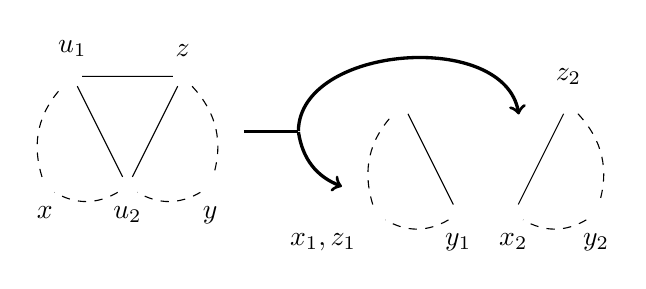
\begin{tikzpicture}[scale=1.4]
    \node (u1) at (0.25cm, 1.25cm) [label=above:${u_1}$] {};
    \node (y) at (1.5cm, 0.25cm) [label=below:${y}$] {};
    \node (z) at (1.25cm, 1.25cm) [label=above:${z}$] {};
    \node (x) at (0.0cm, 0.25cm) [label=below:${x}$] {};
    \node (v) at (0.75cm, 0.25cm) [label=below:${u_2}$] {};

    \begin{pgfonlayer}{bg}
        \draw (z) edge (u1);
        \draw (z) edge (v);
        \draw (u1) edge (v);
        \draw (z) edge [dashed, bend left] (y);
        \draw (y) edge [dashed, bend left] (v);
        \draw (v) edge [dashed, bend left] (x);
        \draw (x) edge [dashed, bend left] (u1);
    \end{pgfonlayer}

    \node (bs) [empty] at (1.8cm, 0.75cm){};
    \node (bm) [empty] at (2.3cm, 0.75cm){};
    \node (be1) [empty] at (4.3cm, 0.9cm){};
    \node (be2) [empty] at (2.7cm, 0.25cm){};

    \draw (bs) edge [very thick] (bm);
    \draw (bm) edge[very thick, ->, bend left=85] (be1);
    \draw (bm) edge[very thick, ->, bend right] (be2);

    \node (u1b) at (3.25cm, 1.0cm) {};
    \node (xb) at (3.0cm, 0.0cm) [label=below left:${x_1,z_1}$] {};
    \node (vb) at (3.75cm, 0.0cm) [label=below:${y_1}$] {};

    \node (zbp) at (4.75cm, 1.0cm) [label=above:${z_2}$] {};
    \node (vbp) at (4.25cm, 0.0cm) [label=below:${x_2}$] {};
    \node (ybp) at (5.0cm, 0.0cm) [label=below:${y_2}$] {};

    \begin{pgfonlayer}{bg}
        \draw (u1b) edge (vb);
        \draw (vb) edge [dashed, bend left] (xb);
        \draw (xb) edge [dashed, bend left] (u1b);

        \draw (zbp) edge (vbp);
        \draw (zbp) edge [dashed, bend left] (ybp);
        \draw (ybp) edge [dashed, bend left] (vbp);
    \end{pgfonlayer}\end{tikzpicture}
\caption{The proof of Lemma~\ref{L:hartman3}, Case~3.2.1 (left) and
Case~3.2.2 (right).}
\end{center}
\end{figure}

\textbf{Case 3.2.1.}
Suppose that $u_2\in C[x,z]$. Observe that $x,y,z\in C_2$.
Apply the inductive hypothesis to produce a path $L$-coloring
$c_2$ of $G_2$ with designated
vertices $x_2=x$, $y_2=y$, and $z_2=z$.
Define $L'(u_2)=\{c_2(u_2)\}$ and $L'(v)=L(v)$ for each
$v\in G_1-u_2$. Apply the inductive hypothesis to produce a path $L'$-coloring
$c_1$ of $G_1$ with the single designated vertex $x_1=y_1=z_1=u_2$. Since 
$\text{deg}_{c_1}(u_2)=0$, it follows that $c$ is a path $L$-coloring of $G$
satisfying the lemma.

\textbf{Case 3.2.2.}
Suppose that $u_2\in C[y,x]-x-y$. Pick $c(u_2)\in L(u_2)-c(z)$. Define
$L'(u_2)=\{c(u_2)\}$ and $L'(v)=L(v)$ for each $v\in G-u_2$. 
Observe that
$x\in C_1$ and $z,y\in C_2$. Apply the inductive hypothesis to produce path
$L'$-coloring $c_1$ of
$G_1$ with designated vertices $x_1=z_1=x$ and $y_1=u_2$.
Then find a path
$L'$-coloring $c_2$ of $G_2$ with designated vertices $x_2=u_2$, $y_2=y$, and
$z_2=z$. Note that $\text{deg}_{c_1}(u_2)\le 1$ and
$\text{deg}_{c_2}(u_2)\le 1$, and thus $c$ is a path $L$-coloring of $G$
satisfying the lemma.

\begin{figure}[ht]
\begin{center}
\SolidGraph
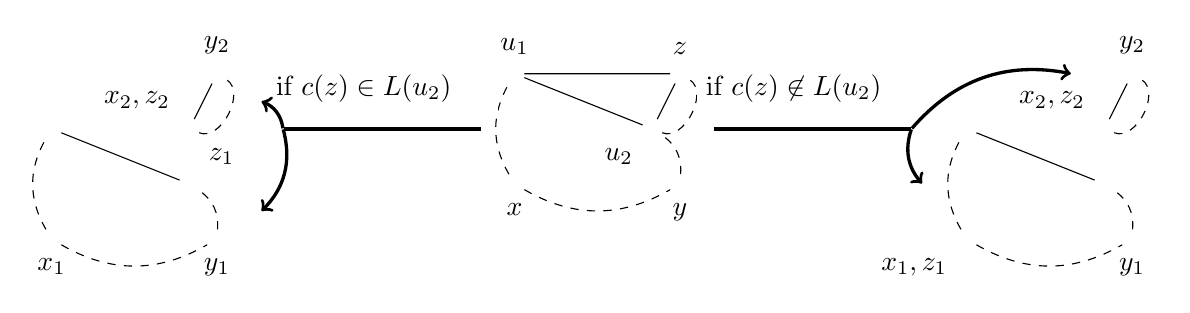
\begin{tikzpicture}[scale=1.4]
    \node (vb) at (-2.95cm, 0.5cm) [label=above left:${x_2,z_2}$] {};
    \node (zb) at (-2.7cm, 1.0cm) [label=above:${y_2}$] {};

    \node (u1bp) at (-4.2cm, 0.5cm) {};
    \node (vbp) at (-2.95cm, 0.0cm) [label=above right:${z_1}$] {};
    \node (xbp) at (-4.2cm, -0.5cm) [label=below:${x_1}$] {};
    \node (ybp) at (-2.7cm, -0.5cm) [label=below:${y_1}$] {};

    \begin{pgfonlayer}{bg}
        \draw (zb) edge (vb);
        \draw (vb) edge [dashed, bend right=85] (zb);

        \draw (vbp) edge (u1bp);
        \draw (ybp) edge [dashed, bend right] (vbp);
        \draw (xbp) edge [dashed, bend left] (u1bp);
        \draw (xbp) edge [dashed, bend right] (ybp);
    \end{pgfonlayer}

    \node (cs) [empty] at (-0.3cm, 0.5cm) {};
    \node (cm) [empty] at (-2.1cm, 0.5cm) {};
    \node (ce1) [empty] at (-2.3cm, 0.75cm) {};
    \node (ce2) [empty] at (-2.3cm, -0.25cm) {};

    \draw (cs) edge [very thick]
        node[above=0.2cm, shape=rectangle, draw=none, fill=white,
                text width=2.7cm]
            {if $c(z)\in L(u_2)$}
        (cm);
    \draw (cm) edge[very thick, ->, bend right] (ce1);
    \draw (cm) edge[very thick, ->, bend left] (ce2);

    \node (u1) at (0.0cm, 1.0cm) [label=above:${u_1}$] {};
    \node (v) at (1.25cm, 0.5cm) [label=below left:${u_2}$] {};
    \node (z) at (1.5cm, 1.0cm) [label=above:${z}$] {};
    \node (x) at (0.0cm, 0.0cm) [label=below:${x}$] {};
    \node (y) at (1.5cm, 0.0cm) [label=below:${y}$] {};

    \begin{pgfonlayer}{bg}
        \draw (z) edge (u1);
        \draw (z) edge (v);
        \draw (u1) edge (v);
        \draw (v) edge [dashed, bend right=85] (z);
        \draw (y) edge [dashed, bend right] (v);
        \draw (x) edge [dashed, bend left] (u1);
        \draw (x) edge [dashed, bend right] (y);
    \end{pgfonlayer}

    \node (bs) [empty] at (1.8cm, 0.5cm) {};
    \node (bm) [empty] at (3.6cm, 0.5cm) {};
    \node (be1) [empty] at (5.05cm, 1.0cm) {};
    \node (be2) [empty] at (3.7cm, 0.0cm) {};

    \draw (bs) edge [very thick]
        node[above=0.2cm, shape=rectangle, draw=none, fill=white,
                text width=2.7cm]
            {if $c(z)\not\in L(u_2)$}
        (bm);
    \draw (bm) edge[very thick, ->, bend left] (be1);
    \draw (bm) edge[very thick, ->, bend right] (be2);

    \node (vb) at (5.35cm, 0.5cm) [label=above left:${x_2,z_2}$] {};
    \node (zb) at (5.6cm, 1.0cm) [label=above:${y_2}$] {};

    \node (u1bp) at (4.1cm, 0.5cm) {};
    \node (vbp) at (5.35cm, 0.0cm) {};
    \node (xbp) at (4.1cm, -0.5cm) [label=below left:${x_1,z_1}$] {};
    \node (ybp) at (5.6cm, -0.5cm) [label=below:${y_1}$] {};

    \begin{pgfonlayer}{bg}
        \draw (zb) edge (vb);
        \draw (vb) edge [dashed, bend right=85] (zb);

        \draw (vbp) edge (u1bp);
        \draw (ybp) edge [dashed, bend right] (vbp);
        \draw (xbp) edge [dashed, bend left] (u1bp);
        \draw (xbp) edge [dashed, bend right] (ybp);
    \end{pgfonlayer}
\end{tikzpicture}
    \caption{The proof of Lemma~\ref{L:hartman3}, Case~3.2.3.}
\end{center}
\end{figure}

\textbf{Case 3.2.3.}
Suppose that $u_2\in C[z,y]$. Note that $z\ne y$. There are two distinct cases to consider.

\textbf{Case 3.2.3.1.} Suppose that $c(z)\in L(u_2)$. Then 
either $u_2=y$ and $L(z)\cap L(y)=\{c(z)\}$, or $C[z,y]\ne z,y$.
Define $L'(u_2)=\{c(z)\}$
and $L'(v)=L(v)$ for each $v\in G-u_2$. Construct a path $L'$-coloring $c_1$ of $G_1$
with designated vertices $x_1=x$,
$y_1=y$, and $z_1=u_2$. Similarly, construct a path $L'$-coloring $c_2$ of
$G_2$ with designated vertices $x_2=u_2$, $y_2=z$, and $z_2=u_2$. Since
$\text{deg}_{c_1}(u_2)\le 1$ and $\text{deg}_{c_2}(u_2)=1$, it follows
that $c$ is a path $L$-coloring of $G$.

\textbf{Case 3.2.3.2.} Suppose that $c(z)\not\in L(u_2)$. Find a path $L$-coloring
$c_1$ of $G_1$ with designated vertices
$x_1=x$, $y_1=y$, and $z_1=x$. Define $L'(u_2)=\{c_1(u_2)\}$ and $L'(v)=L(v)$
for each $v\in G_2-u_2$. Find a path $L'$-coloring $c_2$ of $G_2$
with designated vertices $x_2=u_2$, $y_2=z$, and $z_2=u_2$. Because
$C[z_2,y_2]=z_2,y_2$ and $L'(z_2)\cap L'(y_2)=\emptyset$, it is
guaranteed that $\text{deg}_{c_2}(u_2)=\text{deg}_{c_2}(z_2)=0$. Thus
$c$ is a path $L$-coloring of $G$.

Suppose that $C[z,y]=z,y$. Then it must be that $u_2=y$ and $k=2$.
Therefore $G_2=C_2=z,y$ and $\text{deg}_c(z)=0$ since
$c(z)\not\in L(u_2)$.\ggcnopf
\end{proof}

Let $G$ be a planar graph and $L$ a list assignment such
that $|L(v)|\ge 3$ for each $v\in G$. Compute a planar embedding and add edges
to produce a triangulated plane graph $G'$. Pick $u\in G'$ to be a vertex
on the outer face and $c(u)\in L(u)$. Define $L'$ to be the list
assignment such that $L'(u)=\{c(u)\}$ and $L'(v)=L(v)$ for $v\in G'-u$.
By Lemma~\ref{L:hartman3} there exists a path $L'$-coloring $c$ of $G'$.
Clearly $c$ is also a path $L$-coloring of $G$.
Therefore Theorem~\ref{T:planar3} follows immediately from 
Lemma~\ref{L:hartman3}.

The proof of Lemma~\ref{L:hartman3} is constructive and may be
implemented as a linear time algorithm for plane graphs represented by
rotation scheme ordered augmented adjacency lists.
We will assume that both forward and backward iteration in augmented adjacency
lists
is a constant time operation.
The
available C implementation represents each augmented adjacency list as an array
of entries, but e.g. a doubly linked list would also suffice~\cite{Bro2017}.

\begin{algorithm}\label{A:hartman_impl}
\textbf{Input.} Let $C$ be a cycle or length $2$ path in a
$2$-connected, weakly triangulated plane graph $G$
with augmented adjacency list representation
$\text{Adj}$. Let $x,y,z\in C$ be
vertices such that $z\in C[x,y]$.

Let $L$ be an array of lists of colors
such that for $v\in\{x,y,z\}$ the list $L[v]$ has length one,
for $v\in C-\{x,y,z\}$ the list $L[v]$ has length two
or three, and for $v\in \text{Int}(C)-C$ the list
$L[v]$ has length three. Furthermore, for each $v\in C[x,z] - z$ assume
that $L[v]$ does not contain the color in $L[z]$.

Let $N$ be an array of pairs of
references such that for each $v\in C$ the pair $N[v]=(r_1,r_2)$ contains
a reference $r_1$ to the $\text{Adj}[v]$ entry for neighbor the
immediately counter-clockwise
from $v$
around $C$, and a reference $r_2$
to the entry for the neighbor immediately clockwise from $v$ around $C$.

Let $S$ be an array of
integers such that if $v\in C$, then $S[v]\ne 0$, and if
$v\in \text{Int}(C)-C$, then $S[v]=0$. Also, if
$v\in C$, then $S[v]=S[x]$ if and only if $v\in C[x,z]-z$. Let $M$
be an array of integers such that if $v\in C$, then $M[S[v]]=S[y]$
if and only if $v\in C[z,y]$.

The concrete input to each call will be the arrays $\text{Adj}$, $L$,
$N$, $S$, and $M$, along with the ordered pair $(x,y,z)$.

\textbf{Output.} For each $v\in\text{Int}(C)$, all but one color will be
removed from the list $L[v]$. The remaining color in each list will represent
a path $L$-coloring of $\text{Int}(C)$
such that $\text{deg}_c(x)\le1$, $\text{deg}_c(y)\le1$, and
$\text{deg}_c(z)\le1$. If $z=y$, or if $C[z,y]=z,y$ and $L[z]$ did
not contain the color in $L[y]$, then $\text{deg}_c(z)=0$.

\textbf{Procedure.} Let $N[z]=(r_1,r_2)$. Define the vertex $u_1$ to be
the neighbor of $z$ corresponding to $r_1$.

\textbf{Base Case.} If $r_1=r_2$, then $C=z,u_1$
is a length $2$ path. If $u_1\ne x$ and $u_1\ne y$, remove the
color in $L[z]$ from $L[u_1]$. If more than one color still remains in
$L[u_1]$, remove arbitrary colors until a single color remains.

\textbf{Recursive Step.} Suppose that $r_1\ne r_2$. Note that
$n(C)>2$ and therefore $C$ is a cycle. Define $u_2$ to be the
neighbor of $z$ immediately counter-clockwise from $u_1$.

\textbf{Case 1.} Suppose that $u_1=y$. In this case it must be that
$z=x$. Assign
$S[x]$ and $S[y]$ new unique marks. Assign $M[S[x]]\leftarrow S[x]$
and $M[S[y]]\leftarrow S[y]$. Make a recursive call with
input $(y, x, y)$.

\textbf{Case 2.} Suppose that $z=x$ and $u_1\ne y$. 
Remove the color in $L[z]$ from $L[u_1]$, and then remove arbitrary
colors from $L[u_1]$ until a single color remains.
Set $S[u_1]$ to be a new unique mark, assign $M[S[u_1]]\leftarrow S[u_1]$,
and make a recursive call with input $(u_1, y, z)$.

\textbf{Case 3.} Suppose that $z\ne x$ and $u_1\ne y$. It is this case that
makes use of the back references in the augmented adjacency list representation.

\textbf{Case 3.1.} Suppose that $S[u_2]=0$, that is, $u_2\in
\text{Int}(C)-C$. Assign $S[u_2]\leftarrow S[x]$ and initialize
$N[u_2]\leftarrow(s_1,s_2)$ where $s_1$ is a reference to the entry
for $u_1$ in $\text{Adj}[u_2]$, and $s_2$ is a reference to the entry
for $z$. Remove the color in $L[z]$ from
$L[u_2]$ and remove the edge $zu_1$ by adjusting
$N[u_1]$ and $N[z]$. Make a recursive call with the same input $(x, y, z)$.

\textbf{Case 3.2.} Suppose that $S[u_2]\ne 0$, that is, $u_2\in C$. Just as in
Case~3.2 of the proof of Lemma~\ref{L:hartman3}, we will separately consider
the two blocks $G_1$ and $G_2$ of $\text{Int}(C)-zu_1$.

It is simple to remove the edge $zu_1$ by adjusting $N[z]$ and $N[u_1]$ to
exclude
the corresponding entries. It remains
to ``split'' the
neighborhood of $u_2$ at the edge $u_2z$ such that the recursive call on $G_1$
considers only the neighbors of $u_2$ counter-clockwise from $z$, and the call
on $G_2$ considers $z$ and all neighbors clockwise from $z$.

Let $N[u_2]=(s_1,s_2)$. Let $s_3$ be a reference to $z$'s entry in
$\text{Adj}[u_2]$ and
$s_3+1$ a reference to the next entry counter-clockwise from $z$ in
$\text{Adj}[u_2]$.
To represent
the subgraph $G_1$, assign
$N[u_2]\leftarrow (s_3+1,s_2)$. To represent the $G_2$,
assign $N[u_2]\leftarrow (s_1,s_3)$.

\textbf{Case 3.2.1.} Suppose that $S[u_2]=S[x]$, i.e. $u_2\in C[x,z]$. Make a
recursive call on $G_2$ with input $(x, y, z)$. Assign
$S[u_2]$ a new
unique mark, set $M[S[u_2]]\leftarrow S[u_2]$, and make a recursive call
on $G_1$ with input $(u_2, u_2, u_2)$.

\textbf{Case 3.2.2.} Suppose that $z\ne x$ and $S[u_2]\ne 0$, but
$S[u_2]\ne S[x]$ and $M[S[u_2]]\ne S[y]$. In other words, suppose that
$u_2\in C[y,x]-x-y$.
First remove the color in $L[z]$ from $L[u_2]$, if it exists, and then remove
arbitrary colors until $L[u_2]$ is of length one. Assign $S[u_2]=S[x]$.
Make a recursive call on $G_1$ with input $(x, u_2, x)$.
Assign $S[u_2]$ a new unique mark and $M[S[u_2]]\leftarrow S[u_2]$.
Make a recursive call on $G_2$ with input $(u_2, y, z)$.

\textbf{Case 3.2.3.} Suppose that $z\ne x$ and $M[S[u_2]]=S[y]$, i.e.
$u_2\in C[z,y]$. There are
two cases to consider.

\textbf{Case 3.2.3.1.} Suppose that the color in $L[z]$ is in $L[u_2]$. Remove
all colors from $L[u_2]$ except for the color in $L[z]$.
Make a recursive call on $G_1$ with input $(x, y, u_2)$.
Then assign $S[z]$ and $S[u_2]$ the same new unique mark, and assign
$M[S[z]]\leftarrow S[z]$. Make a
recursive call on $G_2$ with input $(u_2, z, u_2)$.

\textbf{Case 3.2.3.2.} Suppose that the color in $L[z]$ is not in $L[u_2]$.
Assign $M[S[x]]\leftarrow S[y]$. Make a recursive call on $G_1$
with input $(x, y, x)$.
Assign $S[z]$ and $S[u_2]$ the same new unique mark, and
set $M[S[z]]\leftarrow S[z]$. Make a
recursive call on $G_2$ with input $(u_2, z, u_2)$.
\end{algorithm}

\begin{figure}
\begin{center}
\OutlineGraph
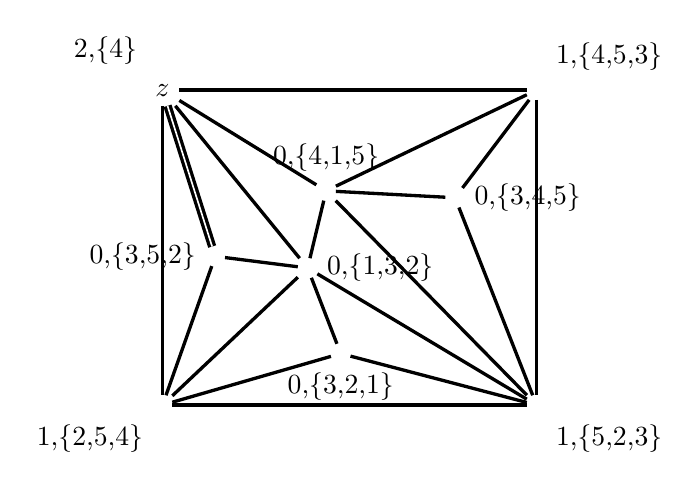
\begin{tikzpicture}
        \node (v0) [label=above left:{2,\{4\}}] at (-2.375000cm, 2.000000cm) {
$z$};
        \node (v1) [label=above right:{1,\{4,5,3\}}] at (2.375000cm, 2.000000c
m) {};
        \node (v2) [label=below right:{1,\{5,2,3\}}] at (2.375000cm, -2.000000
cm) {};
        \node (v3) [label=below left:{1,\{2,5,4\}}] at (-2.375000cm, -2.000000
cm) {};
        \node (v4) [label=right:{0,\{1,3,2\}}] at (-0.532660cm, -0.259649cm) {
};
        \node (v5) [label=above:{0,\{4,1,5\}}] at (-0.297357cm, 0.720239cm) {}
;
        \node (v6) [label=below:{0,\{3,2,1\}}] at (-0.112185cm, -1.346142cm) {
};
        \node (v7) [label=right:{0,\{3,4,5\}}] at (1.340525cm, 0.632695cm) {};
        \node (v8) [label=left:{0,\{3,5,2\}}] at (-1.705649cm, -0.111242cm) {}
;
        \begin{pgfonlayer}{bg}
                \draw (v0) edge [double, very thick] (v8);
                \draw (v0) edge [very thick] (v3);
                \draw (v0) edge [very thick] (v4);
                \draw (v0) edge [very thick] (v5);
                \draw (v0) edge [very thick] (v1);
                \draw (v1) edge [very thick] (v5);
                \draw (v1) edge [very thick] (v7);
                \draw (v1) edge [very thick] (v2);
                \draw (v2) edge [very thick] (v7);
                \draw (v2) edge [very thick] (v5);
                \draw (v2) edge [very thick] (v4);
                \draw (v2) edge [very thick] (v6);
                \draw (v2) edge [very thick] (v3);
                \draw (v3) edge [very thick] (v6);
                \draw (v3) edge [very thick] (v4);
                \draw (v3) edge [very thick] (v8);
                \draw (v4) edge [very thick] (v5);
                \draw (v4) edge [very thick] (v8);
                \draw (v4) edge [very thick] (v6);
                \draw (v5) edge [very thick] (v7);
        \end{pgfonlayer}
\end{tikzpicture}
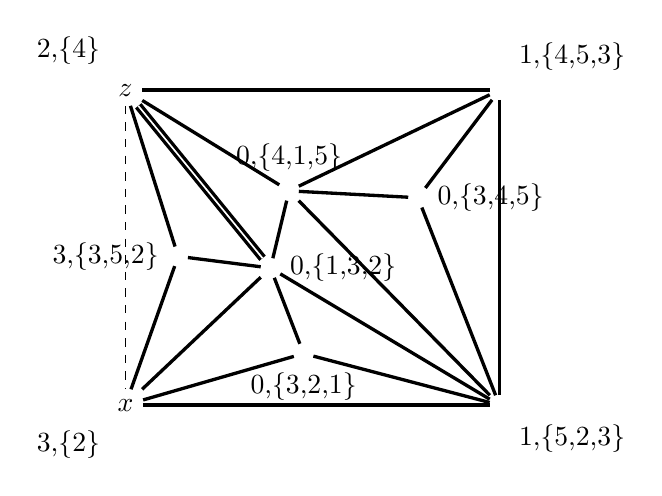
\begin{tikzpicture}
        \node (v0) [label=above left:{2,\{4\}}] at (-2.375000cm, 2.000000cm) {
$z$};
        \node (v1) [label=above right:{1,\{4,5,3\}}] at (2.375000cm, 2.000000c
m) {};
        \node (v2) [label=below right:{1,\{5,2,3\}}] at (2.375000cm, -2.000000
cm) {};
        \node (v3) [label=below left:{3,\{2\}}] at (-2.375000cm, -2.000000cm) 
{$x$};
        \node (v4) [label=right:{0,\{1,3,2\}}] at (-0.532660cm, -0.259649cm) {
};
        \node (v5) [label=above:{0,\{4,1,5\}}] at (-0.297357cm, 0.720239cm) {}
;
        \node (v6) [label=below:{0,\{3,2,1\}}] at (-0.112185cm, -1.346142cm) {
};
        \node (v7) [label=right:{0,\{3,4,5\}}] at (1.340525cm, 0.632695cm) {};
        \node (v8) [label=left:{3,\{3,5,2\}}] at (-1.705649cm, -0.111242cm) {}
;
        \begin{pgfonlayer}{bg}
                \draw (v0) edge [double, very thick] (v4);
                \draw (v0) edge [very thick] (v8);
                \draw (v0) edge [very thick] (v5);
                \draw (v0) edge [very thick] (v1);
                \draw (v1) edge [very thick] (v5);
                \draw (v1) edge [very thick] (v7);
                \draw (v1) edge [very thick] (v2);
                \draw (v2) edge [very thick] (v7);
                \draw (v2) edge [very thick] (v5);
                \draw (v2) edge [very thick] (v4);
                \draw (v2) edge [very thick] (v6);
                \draw (v2) edge [very thick] (v3);
                \draw (v3) edge [very thick] (v6);
                \draw (v3) edge [very thick] (v4);
                \draw (v3) edge [very thick] (v8);
                \draw (v0) edge [dashed] (v3);
                \draw (v4) edge [very thick] (v5);
                \draw (v4) edge [very thick] (v8);
                \draw (v4) edge [very thick] (v6);
                \draw (v5) edge [very thick] (v7);
        \end{pgfonlayer}
\end{tikzpicture}

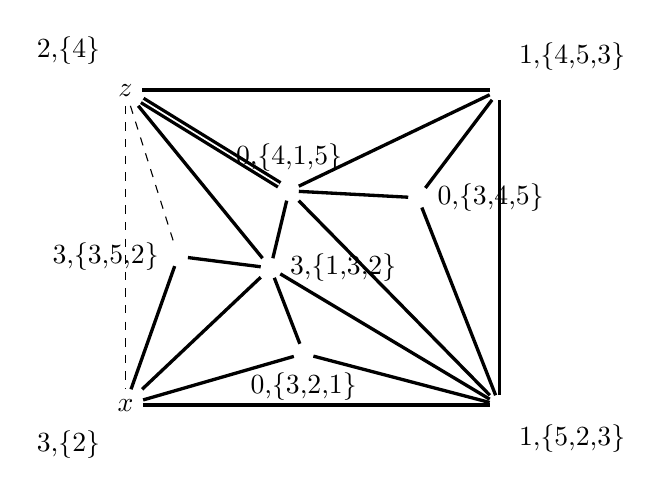
\begin{tikzpicture}
        \node (v0) [label=above left:{2,\{4\}}] at (-2.375000cm, 2.000000cm) {
$z$};
        \node (v1) [label=above right:{1,\{4,5,3\}}] at (2.375000cm, 2.000000c
m) {};
        \node (v2) [label=below right:{1,\{5,2,3\}}] at (2.375000cm, -2.000000
cm) {};
        \node (v3) [label=below left:{3,\{2\}}] at (-2.375000cm, -2.000000cm) 
{$x$};
        \node (v4) [label=right:{3,\{1,3,2\}}] at (-0.532660cm, -0.259649cm) {
};
        \node (v5) [label=above:{0,\{4,1,5\}}] at (-0.297357cm, 0.720239cm) {}
;
        \node (v6) [label=below:{0,\{3,2,1\}}] at (-0.112185cm, -1.346142cm) {
};
        \node (v7) [label=right:{0,\{3,4,5\}}] at (1.340525cm, 0.632695cm) {};
        \node (v8) [label=left:{3,\{3,5,2\}}] at (-1.705649cm, -0.111242cm) {}
;
        \begin{pgfonlayer}{bg}
                \draw (v0) edge [double, very thick] (v5);
                \draw (v0) edge [very thick] (v4);
                \draw (v0) edge [very thick] (v1);
                \draw (v1) edge [very thick] (v5);
                \draw (v1) edge [very thick] (v7);
                \draw (v1) edge [very thick] (v2);
                \draw (v2) edge [very thick] (v7);
                \draw (v2) edge [very thick] (v5);
                \draw (v2) edge [very thick] (v4);
                \draw (v2) edge [very thick] (v6);
                \draw (v2) edge [very thick] (v3);
                \draw (v3) edge [very thick] (v6);
                \draw (v3) edge [very thick] (v4);
                \draw (v3) edge [very thick] (v8);
                \draw (v4) edge [very thick] (v8);
                \draw (v4) edge [very thick] (v6);
                \draw (v4) edge [very thick] (v5);
                \draw (v0) edge [dashed] (v3);
                \draw (v0) edge [dashed] (v8);
                \draw (v5) edge [very thick] (v7);
        \end{pgfonlayer}
\end{tikzpicture}
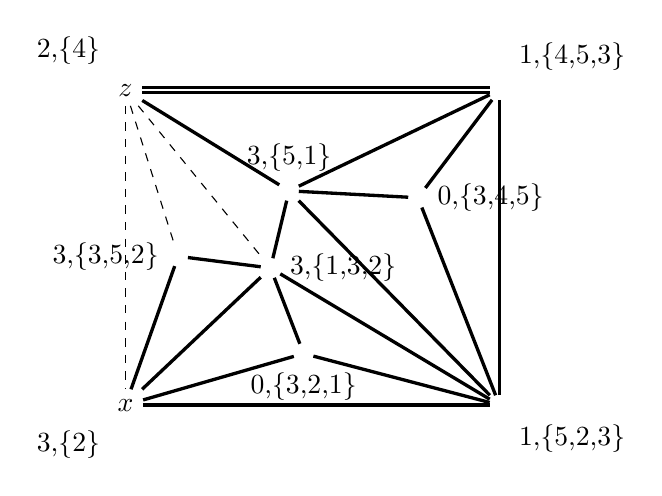
\begin{tikzpicture}
        \node (v0) [label=above left:{2,\{4\}}] at (-2.375000cm, 2.000000cm) {
$z$};
        \node (v1) [label=above right:{1,\{4,5,3\}}] at (2.375000cm, 2.000000c
m) {};
        \node (v2) [label=below right:{1,\{5,2,3\}}] at (2.375000cm, -2.000000
cm) {};
        \node (v3) [label=below left:{3,\{2\}}] at (-2.375000cm, -2.000000cm) 
{$x$};
        \node (v4) [label=right:{3,\{1,3,2\}}] at (-0.532660cm, -0.259649cm) {
};
        \node (v5) [label=above:{3,\{5,1\}}] at (-0.297357cm, 0.720239cm) {};
        \node (v6) [label=below:{0,\{3,2,1\}}] at (-0.112185cm, -1.346142cm) {
};
        \node (v7) [label=right:{0,\{3,4,5\}}] at (1.340525cm, 0.632695cm) {};
        \node (v8) [label=left:{3,\{3,5,2\}}] at (-1.705649cm, -0.111242cm) {}
;
        \begin{pgfonlayer}{bg}
                \draw (v0) edge [double, very thick] (v1);
                \draw (v0) edge [very thick] (v5);
                \draw (v1) edge [very thick] (v5);
                \draw (v1) edge [very thick] (v7);
                \draw (v1) edge [very thick] (v2);
                \draw (v2) edge [very thick] (v7);
                \draw (v2) edge [very thick] (v5);
                \draw (v2) edge [very thick] (v4);
                \draw (v2) edge [very thick] (v6);
                \draw (v2) edge [very thick] (v3);
                \draw (v3) edge [very thick] (v6);
                \draw (v3) edge [very thick] (v4);
                \draw (v3) edge [very thick] (v8);
                \draw (v4) edge [very thick] (v8);
                \draw (v4) edge [very thick] (v6);
                \draw (v4) edge [very thick] (v5);
                \draw (v5) edge [very thick] (v7);
                \draw (v0) edge [dashed] (v3);
                \draw (v0) edge [dashed] (v8);
                \draw (v0) edge [dashed] (v4);
        \end{pgfonlayer}
\end{tikzpicture}

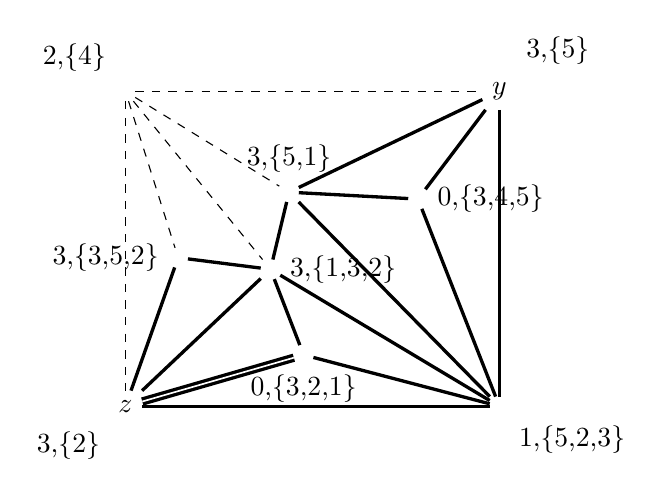
\begin{tikzpicture}
        \node (v0) [label=above left:{2,\{4\}}] at (-2.375000cm, 2.000000cm) {
};
        \node (v1) [label=above right:{3,\{5\}}] at (2.375000cm, 2.000000cm) {
$y$};
        \node (v2) [label=below right:{1,\{5,2,3\}}] at (2.375000cm, -2.000000
cm) {};
        \node (v3) [label=below left:{3,\{2\}}] at (-2.375000cm, -2.000000cm) 
{$z$};
        \node (v4) [label=right:{3,\{1,3,2\}}] at (-0.532660cm, -0.259649cm) {
};
        \node (v5) [label=above:{3,\{5,1\}}] at (-0.297357cm, 0.720239cm) {};
        \node (v6) [label=below:{0,\{3,2,1\}}] at (-0.112185cm, -1.346142cm) {
};
        \node (v7) [label=right:{0,\{3,4,5\}}] at (1.340525cm, 0.632695cm) {};
        \node (v8) [label=left:{3,\{3,5,2\}}] at (-1.705649cm, -0.111242cm) {}
;
        \begin{pgfonlayer}{bg}
                \draw (v3) edge [double, very thick] (v6);
                \draw (v3) edge [very thick] (v4);
                \draw (v3) edge [very thick] (v8);
                \draw (v4) edge [very thick] (v8);
                \draw (v4) edge [very thick] (v6);
                \draw (v4) edge [very thick] (v5);
                \draw (v5) edge [very thick] (v7);
                \draw (v1) edge [very thick] (v5);
                \draw (v1) edge [very thick] (v7);
                \draw (v1) edge [very thick] (v2);
                \draw (v2) edge [very thick] (v7);
                \draw (v2) edge [very thick] (v5);
                \draw (v2) edge [very thick] (v4);
                \draw (v2) edge [very thick] (v6);
                \draw (v2) edge [very thick] (v3);
                \draw (v0) edge [dashed] (v3);
                \draw (v0) edge [dashed] (v8);
                \draw (v0) edge [dashed] (v4);
                \draw (v0) edge [dashed] (v5);
                \draw (v0) edge [dashed] (v1);
        \end{pgfonlayer}
\end{tikzpicture}
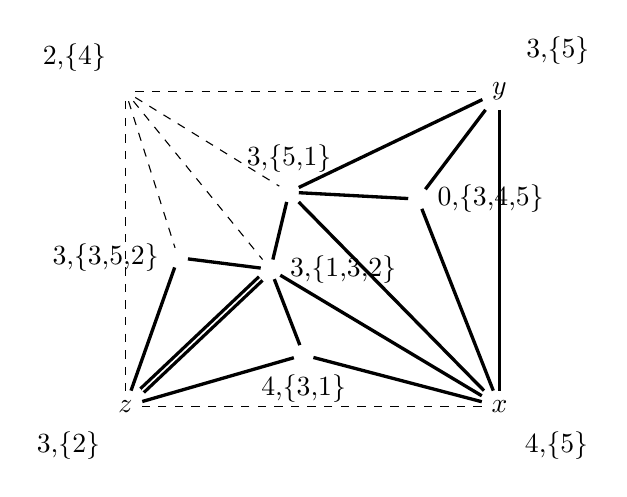
\begin{tikzpicture}
        \node (v0) [label=above left:{2,\{4\}}] at (-2.375000cm, 2.000000cm) {
};
        \node (v1) [label=above right:{3,\{5\}}] at (2.375000cm, 2.000000cm) {
$y$};
        \node (v2) [label=below right:{4,\{5\}}] at (2.375000cm, -2.000000cm) 
{$x$};
        \node (v3) [label=below left:{3,\{2\}}] at (-2.375000cm, -2.000000cm) 
{$z$};
        \node (v4) [label=right:{3,\{1,3,2\}}] at (-0.532660cm, -0.259649cm) {
};
        \node (v5) [label=above:{3,\{5,1\}}] at (-0.297357cm, 0.720239cm) {};
        \node (v6) [label=below:{4,\{3,1\}}] at (-0.112185cm, -1.346142cm) {};
        \node (v7) [label=right:{0,\{3,4,5\}}] at (1.340525cm, 0.632695cm) {};
        \node (v8) [label=left:{3,\{3,5,2\}}] at (-1.705649cm, -0.111242cm) {}
;
        \begin{pgfonlayer}{bg}
                \draw (v3) edge [double, very thick] (v4);
                \draw (v3) edge [very thick] (v6);
                \draw (v3) edge [very thick] (v8);
                \draw (v4) edge [very thick] (v8);
                \draw (v4) edge [very thick] (v6);
                \draw (v4) edge [very thick] (v5);
                \draw (v5) edge [very thick] (v7);
                \draw (v1) edge [very thick] (v5);
                \draw (v1) edge [very thick] (v7);
                \draw (v1) edge [very thick] (v2);
                \draw (v2) edge [very thick] (v7);
                \draw (v2) edge [very thick] (v5);
                \draw (v2) edge [very thick] (v4);
                \draw (v2) edge [very thick] (v6);
                \draw (v0) edge [dashed] (v3);
                \draw (v0) edge [dashed] (v8);
                \draw (v0) edge [dashed] (v4);
                \draw (v0) edge [dashed] (v5);
                \draw (v0) edge [dashed] (v1);
                \draw (v2) edge [dashed] (v3);
        \end{pgfonlayer}
\end{tikzpicture}

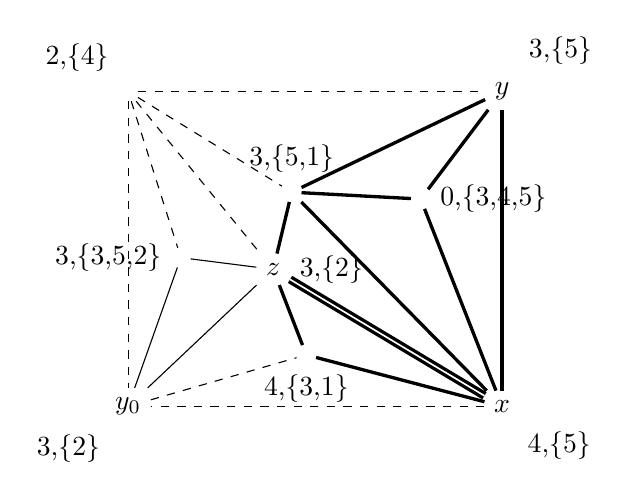
\begin{tikzpicture}
        \node (v0) [label=above left:{2,\{4\}}] at (-2.375000cm, 2.000000cm) {
};
        \node (v1) [label=above right:{3,\{5\}}] at (2.375000cm, 2.000000cm) {
$y$};
        \node (v2) [label=below right:{4,\{5\}}] at (2.375000cm, -2.000000cm) 
{$x$};
        \node (v3) [label=below left:{3,\{2\}}] at (-2.375000cm, -2.000000cm) 
{$y_{0}$};
        \node (v4) [label=right:{3,\{2\}}] at (-0.532660cm, -0.259649cm) {$z$}
;
        \node (v5) [label=above:{3,\{5,1\}}] at (-0.297357cm, 0.720239cm) {};
        \node (v6) [label=below:{4,\{3,1\}}] at (-0.112185cm, -1.346142cm) {};
        \node (v7) [label=right:{0,\{3,4,5\}}] at (1.340525cm, 0.632695cm) {};
        \node (v8) [label=left:{3,\{3,5,2\}}] at (-1.705649cm, -0.111242cm) {}
;
        \begin{pgfonlayer}{bg}
                \draw (v2) edge [double, very thick] (v4);
                \draw (v4) edge [very thick] (v6);
                \draw (v4) edge [very thick] (v5);
                \draw (v5) edge [very thick] (v7);
                \draw (v1) edge [very thick] (v5);
                \draw (v1) edge [very thick] (v7);
                \draw (v1) edge [very thick] (v2);
                \draw (v2) edge [very thick] (v7);
                \draw (v2) edge [very thick] (v5);
                \draw (v2) edge [very thick] (v6);
                \draw (v4) edge [thin] (v8);
                \draw (v3) edge [thin] (v4);
                \draw (v3) edge [thin] (v8);
                \draw (v0) edge [dashed] (v3);
                \draw (v0) edge [dashed] (v8);
                \draw (v0) edge [dashed] (v4);
                \draw (v0) edge [dashed] (v5);
                \draw (v0) edge [dashed] (v1);
                \draw (v2) edge [dashed] (v3);
                \draw (v3) edge [dashed] (v6);
        \end{pgfonlayer}
\end{tikzpicture}
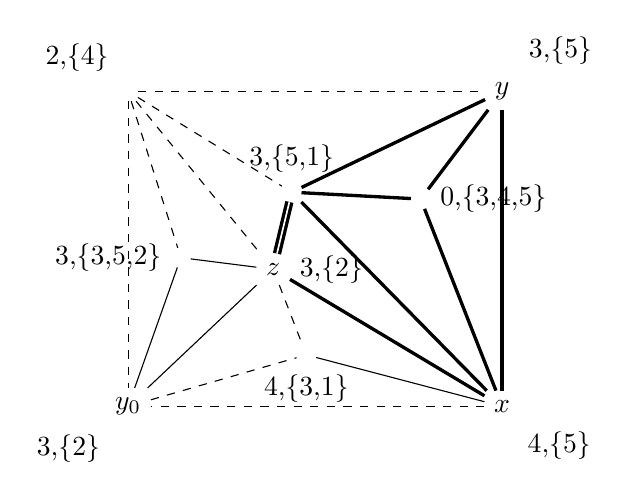
\begin{tikzpicture}
        \node (v0) [label=above left:{2,\{4\}}] at (-2.375000cm, 2.000000cm) {
};
        \node (v1) [label=above right:{3,\{5\}}] at (2.375000cm, 2.000000cm) {
$y$};
        \node (v2) [label=below right:{4,\{5\}}] at (2.375000cm, -2.000000cm) 
{$x$};
        \node (v3) [label=below left:{3,\{2\}}] at (-2.375000cm, -2.000000cm) 
{$y_{0}$};
        \node (v4) [label=right:{3,\{2\}}] at (-0.532660cm, -0.259649cm) {$z$}
;
        \node (v5) [label=above:{3,\{5,1\}}] at (-0.297357cm, 0.720239cm) {};
        \node (v6) [label=below:{4,\{3,1\}}] at (-0.112185cm, -1.346142cm) {};
        \node (v7) [label=right:{0,\{3,4,5\}}] at (1.340525cm, 0.632695cm) {};
        \node (v8) [label=left:{3,\{3,5,2\}}] at (-1.705649cm, -0.111242cm) {}
;
        \begin{pgfonlayer}{bg}
                \draw (v4) edge [double, very thick] (v5);
                \draw (v5) edge [very thick](v7);
                \draw (v1) edge [very thick](v5);
                \draw (v1) edge [very thick](v7);
                \draw (v1) edge [very thick](v2);
                \draw (v2) edge [very thick](v7);
                \draw (v2) edge [very thick](v5);
                \draw (v2) edge [very thick](v4);
                \draw (v4) edge [thin] (v8);
                \draw (v3) edge [thin] (v4);
                \draw (v3) edge [thin] (v8);
                \draw (v2) edge [thin] (v6);
                \draw (v0) edge [dashed] (v3);
                \draw (v0) edge [dashed] (v8);
                \draw (v0) edge [dashed] (v4);
                \draw (v0) edge [dashed] (v5);
                \draw (v0) edge [dashed] (v1);
                \draw (v2) edge [dashed] (v3);
                \draw (v3) edge [dashed] (v6);
                \draw (v4) edge [dashed] (v6);
        \end{pgfonlayer}
\end{tikzpicture}
\caption{An example of Algorithm~\ref{A:hartman_impl}. Each vertex $v\in G$ is labelled with $S[v],L[v]$.}
\label{F:hartman_impl}
\end{center}
\end{figure}

\begin{figure}
\begin{center}
\OutlineGraph
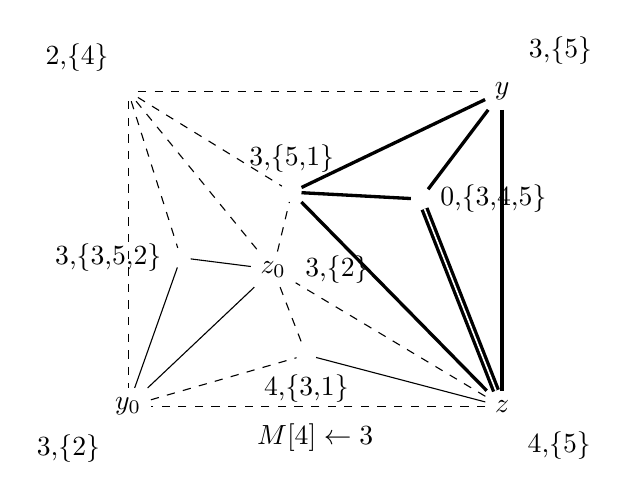
\begin{tikzpicture}
        \node (v0) [label=above left:{2,\{4\}}] at (-2.375000cm, 2.000000cm) {
};
        \node (v1) [label=above right:{3,\{5\}}] at (2.375000cm, 2.000000cm) {
$y$};
        \node (v2) [label=below right:{4,\{5\}}] at (2.375000cm, -2.000000cm) 
{$z$};
        \node (v3) [label=below left:{3,\{2\}}] at (-2.375000cm, -2.000000cm) 
{$y_{0}$};
        \node (v4) [label=right:{3,\{2\}}] at (-0.532660cm, -0.259649cm) {$z_{
0}$};
        \node (v5) [label=above:{3,\{5,1\}}] at (-0.297357cm, 0.720239cm) {};
        \node (v6) [label=below:{4,\{3,1\}}] at (-0.112185cm, -1.346142cm) {};
        \node (v7) [label=right:{0,\{3,4,5\}}] at (1.340525cm, 0.632695cm) {};
        \node (v8) [label=left:{3,\{3,5,2\}}] at (-1.705649cm, -0.111242cm) {};

        \node (M) [shape=rectangle, draw=none, fill=white] at (0.0cm, -2.4cm) {$M[4]\leftarrow 3$};

        \begin{pgfonlayer}{bg}
                \draw (v2) edge [double, very thick] (v7);
                \draw (v2) edge [very thick] (v5);
                \draw (v5) edge [very thick] (v7);
                \draw (v1) edge [very thick] (v5);
                \draw (v1) edge [very thick] (v7);
                \draw (v1) edge [very thick] (v2);
                \draw (v4) edge [thin] (v8);
                \draw (v3) edge [thin] (v4);
                \draw (v3) edge [thin] (v8);
                \draw (v2) edge [thin] (v6);
                \draw (v0) edge [dashed] (v3);
                \draw (v0) edge [dashed] (v8);
                \draw (v0) edge [dashed] (v4);
                \draw (v0) edge [dashed] (v5);
                \draw (v0) edge [dashed] (v1);
                \draw (v2) edge [dashed] (v4);
                \draw (v2) edge [dashed] (v3);
                \draw (v3) edge [dashed] (v6);
                \draw (v4) edge [dashed] (v5);
                \draw (v4) edge [dashed] (v6);
        \end{pgfonlayer}
\end{tikzpicture}
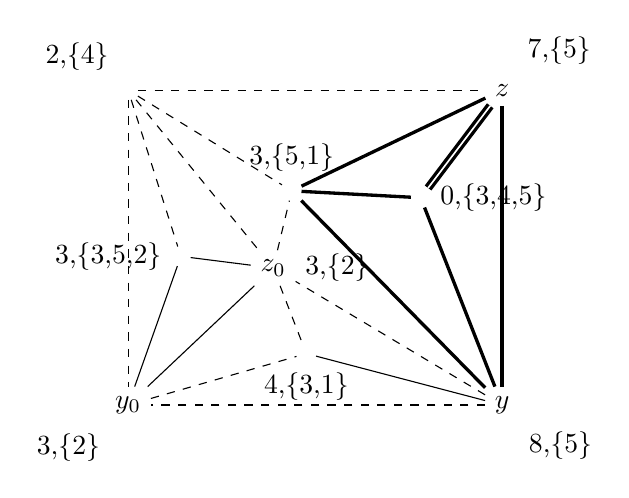
\begin{tikzpicture}
        \node (v0) [label=above left:{2,\{4\}}] at (-2.375000cm, 2.000000cm) {
};
        \node (v1) [label=above right:{7,\{5\}}] at (2.375000cm, 2.000000cm) {
$z$};
        \node (v2) [label=below right:{8,\{5\}}] at (2.375000cm, -2.000000cm) 
{$y$};
        \node (v3) [label=below left:{3,\{2\}}] at (-2.375000cm, -2.000000cm) 
{$y_{0}$};
        \node (v4) [label=right:{3,\{2\}}] at (-0.532660cm, -0.259649cm) {$z_{
0}$};
        \node (v5) [label=above:{3,\{5,1\}}] at (-0.297357cm, 0.720239cm) {};
        \node (v6) [label=below:{4,\{3,1\}}] at (-0.112185cm, -1.346142cm) {};
        \node (v7) [label=right:{0,\{3,4,5\}}] at (1.340525cm, 0.632695cm) {};
        \node (v8) [label=left:{3,\{3,5,2\}}] at (-1.705649cm, -0.111242cm) {}
;
        \begin{pgfonlayer}{bg}
                \draw (v1) edge [double, very thick] (v7);
                \draw (v1) edge [very thick] (v5);
                \draw (v1) edge [very thick] (v2);
                \draw (v2) edge [very thick] (v7);
                \draw (v2) edge [very thick] (v5);
                \draw (v5) edge [very thick] (v7);
                \draw (v4) edge [thin] (v8);
                \draw (v3) edge [thin] (v4);
                \draw (v3) edge [thin] (v8);
                \draw (v2) edge [thin] (v6);
                \draw (v0) edge [dashed] (v3);
                \draw (v0) edge [dashed] (v8);
                \draw (v0) edge [dashed] (v4);
                \draw (v0) edge [dashed] (v5);
                \draw (v0) edge [dashed] (v1);
                \draw (v2) edge [dashed] (v4);
                \draw (v2) edge [dashed] (v3);
                \draw (v3) edge [dashed] (v6);
                \draw (v4) edge [dashed] (v5);
                \draw (v4) edge [dashed] (v6);
        \end{pgfonlayer}
\end{tikzpicture}

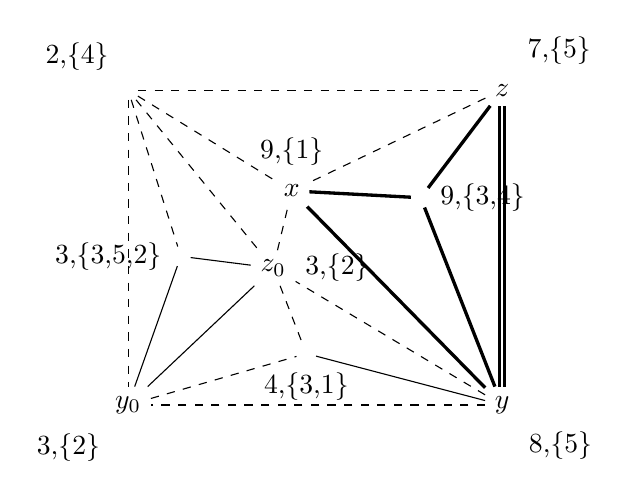
\begin{tikzpicture}
        \node (v0) [label=above left:{2,\{4\}}] at (-2.375000cm, 2.000000cm) {
};
        \node (v1) [label=above right:{7,\{5\}}] at (2.375000cm, 2.000000cm) {
$z$};
        \node (v2) [label=below right:{8,\{5\}}] at (2.375000cm, -2.000000cm) 
{$y$};
        \node (v3) [label=below left:{3,\{2\}}] at (-2.375000cm, -2.000000cm) 
{$y_{0}$};
        \node (v4) [label=right:{3,\{2\}}] at (-0.532660cm, -0.259649cm) {$z_{
0}$};
        \node (v5) [label=above:{9,\{1\}}] at (-0.297357cm, 0.720239cm) {$x$};
        \node (v6) [label=below:{4,\{3,1\}}] at (-0.112185cm, -1.346142cm) {};
        \node (v7) [label=right:{9,\{3,4\}}] at (1.340525cm, 0.632695cm) {};
        \node (v8) [label=left:{3,\{3,5,2\}}] at (-1.705649cm, -0.111242cm) {}
;
        \begin{pgfonlayer}{bg}
                \draw (v1) edge [double, very thick] (v2);
                \draw (v1) edge [very thick] (v7);
                \draw (v2) edge [very thick] (v7);
                \draw (v2) edge [very thick] (v5);
                \draw (v5) edge [very thick] (v7);
                \draw (v4) edge [thin] (v8);
                \draw (v3) edge [thin] (v4);
                \draw (v3) edge [thin] (v8);
                \draw (v2) edge [thin] (v6);
                \draw (v0) edge [dashed] (v3);
                \draw (v0) edge [dashed] (v8);
                \draw (v0) edge [dashed] (v4);
                \draw (v0) edge [dashed] (v5);
                \draw (v0) edge [dashed] (v1);
                \draw (v1) edge [dashed] (v5);
                \draw (v2) edge [dashed] (v4);
                \draw (v2) edge [dashed] (v3);
                \draw (v3) edge [dashed] (v6);
                \draw (v4) edge [dashed] (v5);
                \draw (v4) edge [dashed] (v6);
        \end{pgfonlayer}
\end{tikzpicture}
\begin{tikzpicture}
        \node (v0) [label=above left:{2,\{4\}}] at (-2.375000cm, 2.000000cm) {
};
        \node (v1) [label=above right:{7,\{5\}}] at (2.375000cm, 2.000000cm) {
};
        \node (v2) [label=below right:{8,\{5\}}] at (2.375000cm, -2.000000cm) 
{$z$};
        \node (v3) [label=below left:{3,\{2\}}] at (-2.375000cm, -2.000000cm) 
{$y_{0}$};
        \node (v4) [label=right:{3,\{2\}}] at (-0.532660cm, -0.259649cm) {$z_{
0}$};
        \node (v5) [label=above:{9,\{1\}}] at (-0.297357cm, 0.720239cm) {$x$};
        \node (v6) [label=below:{4,\{3,1\}}] at (-0.112185cm, -1.346142cm) {};
        \node (v7) [label=right:{9,\{3,4\}}] at (1.340525cm, 0.632695cm) {};
        \node (v8) [label=left:{3,\{3,5,2\}}] at (-1.705649cm, -0.111242cm) {}
;
        \begin{pgfonlayer}{bg}
                \draw (v2) edge [double, very thick] (v5);
                \draw (v2) edge [very thick] (v7);
                \draw (v5) edge [very thick] (v7);
                \draw (v4) edge [thin] (v8);
                \draw (v3) edge [thin] (v4);
                \draw (v3) edge [thin] (v8);
                \draw (v2) edge [thin] (v6);
                \draw (v0) edge [dashed] (v3);
                \draw (v0) edge [dashed] (v8);
                \draw (v0) edge [dashed] (v4);
                \draw (v0) edge [dashed] (v5);
                \draw (v0) edge [dashed] (v1);
                \draw (v1) edge [dashed] (v5);
                \draw (v1) edge [dashed] (v7);
                \draw (v1) edge [dashed] (v2);
                \draw (v2) edge [dashed] (v4);
                \draw (v2) edge [dashed] (v3);
                \draw (v3) edge [dashed] (v6);
                \draw (v4) edge [dashed] (v5);
                \draw (v4) edge [dashed] (v6);
        \end{pgfonlayer}
\end{tikzpicture}

\begin{tikzpicture}
        \node (v0) [label=above left:{2,\{4\}}] at (-2.375000cm, 2.000000cm) {
};
        \node (v1) [label=above right:{7,\{5\}}] at (2.375000cm, 2.000000cm) {
};
        \node (v2) [label=below right:{8,\{5\}}] at (2.375000cm, -2.000000cm) 
{$z_{1}$};
        \node (v3) [label=below left:{3,\{2\}}] at (-2.375000cm, -2.000000cm) 
{$y_{0}$};
        \node (v4) [label=right:{3,\{2\}}] at (-0.532660cm, -0.259649cm) {$z_{
0}$};
        \node (v5) [label=above:{10,\{1\}}] at (-0.297357cm, 0.720239cm) {$z$}
;
        \node (v6) [label=below:{4,\{3,1\}}] at (-0.112185cm, -1.346142cm) {};
        \node (v7) [label=right:{9,\{3,4\}}] at (1.340525cm, 0.632695cm) {};
        \node (v8) [label=left:{3,\{3,5,2\}}] at (-1.705649cm, -0.111242cm) {}
;
        \begin{pgfonlayer}{bg}
                \draw (v5) edge [double, very thick] (v7);
                \draw (v4) edge [thin] (v8);
                \draw (v3) edge [thin] (v4);
                \draw (v3) edge [thin] (v8);
                \draw (v2) edge [thin] (v6);
                \draw (v0) edge [dashed] (v3);
                \draw (v0) edge [dashed] (v8);
                \draw (v0) edge [dashed] (v4);
                \draw (v0) edge [dashed] (v5);
                \draw (v0) edge [dashed] (v1);
                \draw (v1) edge [dashed] (v5);
                \draw (v1) edge [dashed] (v7);
                \draw (v1) edge [dashed] (v2);
                \draw (v2) edge [dashed] (v7);
                \draw (v2) edge [dashed] (v5);
                \draw (v2) edge [dashed] (v4);
                \draw (v2) edge [dashed] (v3);
                \draw (v3) edge [dashed] (v6);
                \draw (v4) edge [dashed] (v5);
                \draw (v4) edge [dashed] (v6);
        \end{pgfonlayer}
\end{tikzpicture}
\begin{tikzpicture}
        \node (v0) [label=above left:{2,\{4\}}] at (-2.375000cm, 2.000000cm) {
};
        \node (v1) [label=above right:{7,\{5\}}] at (2.375000cm, 2.000000cm) {
};
        \node (v2) [label=below right:{6,\{5\}}] at (2.375000cm, -2.000000cm) 
{$z$};
        \node (v3) [label=below left:{3,\{2\}}] at (-2.375000cm, -2.000000cm) 
{$y_{0}$};
        \node (v4) [label=right:{3,\{2\}}] at (-0.532660cm, -0.259649cm) {$z_{
0}$};
        \node (v5) [label=above:{10,\{1\}}] at (-0.297357cm, 0.720239cm) {};
        \node (v6) [label=below:{4,\{3,1\}}] at (-0.112185cm, -1.346142cm) {};
        \node (v7) [label=right:{9,\{3\}}] at (1.340525cm, 0.632695cm) {};
        \node (v8) [label=left:{3,\{3,5,2\}}] at (-1.705649cm, -0.111242cm) {}
;
        \begin{pgfonlayer}{bg}
                \draw (v2) edge [double, very thick] (v6);
                \draw (v4) edge [thin] (v8);
                \draw (v3) edge [thin] (v4);
                \draw (v3) edge [thin] (v8);
                \draw (v0) edge [dashed] (v3);
                \draw (v0) edge [dashed] (v8);
                \draw (v0) edge [dashed] (v4);
                \draw (v0) edge [dashed] (v5);
                \draw (v0) edge [dashed] (v1);
                \draw (v1) edge [dashed] (v5);
                \draw (v1) edge [dashed] (v7);
                \draw (v1) edge [dashed] (v2);
                \draw (v2) edge [dashed] (v7);
                \draw (v2) edge [dashed] (v5);
                \draw (v2) edge [dashed] (v4);
                \draw (v2) edge [dashed] (v3);
                \draw (v3) edge [dashed] (v6);
                \draw (v4) edge [dashed] (v5);
                \draw (v4) edge [dashed] (v6);
                \draw (v5) edge [dashed] (v7);
        \end{pgfonlayer}
\end{tikzpicture}

\begin{tikzpicture}
        \node (v0) [label=above left:{2,\{4\}}] at (-2.375000cm, 2.000000cm) {
};
        \node (v1) [label=above right:{7,\{5\}}] at (2.375000cm, 2.000000cm) {
};
        \node (v2) [label=below right:{6,\{5\}}] at (2.375000cm, -2.000000cm) 
{};
        \node (v3) [label=below left:{5,\{2\}}] at (-2.375000cm, -2.000000cm) 
{$y$};
        \node (v4) [label=right:{5,\{2\}}] at (-0.532660cm, -0.259649cm) {$z$}
;
        \node (v5) [label=above:{10,\{1\}}] at (-0.297357cm, 0.720239cm) {};
        \node (v6) [label=below:{4,\{3\}}] at (-0.112185cm, -1.346142cm) {};
        \node (v7) [label=right:{9,\{3\}}] at (1.340525cm, 0.632695cm) {};
        \node (v8) [label=left:{3,\{3,5,2\}}] at (-1.705649cm, -0.111242cm) {}
;
        \begin{pgfonlayer}{bg}
                \draw (v3) edge [double, very thick] (v4);
                \draw (v4) edge [very thick] (v8);
                \draw (v3) edge [very thick] (v8);
                \draw (v0) edge [dashed] (v3);
                \draw (v0) edge [dashed] (v8);
                \draw (v0) edge [dashed] (v4);
                \draw (v0) edge [dashed] (v5);
                \draw (v0) edge [dashed] (v1);
                \draw (v1) edge [dashed] (v5);
                \draw (v1) edge [dashed] (v7);
                \draw (v1) edge [dashed] (v2);
                \draw (v2) edge [dashed] (v7);
                \draw (v2) edge [dashed] (v5);
                \draw (v2) edge [dashed] (v4);
                \draw (v2) edge [dashed] (v6);
                \draw (v2) edge [dashed] (v3);
                \draw (v3) edge [dashed] (v6);
                \draw (v4) edge [dashed] (v5);
                \draw (v4) edge [dashed] (v6);
                \draw (v5) edge [dashed] (v7);
        \end{pgfonlayer}
\end{tikzpicture}
\begin{tikzpicture}
        \node (v0) [label=above left:{2,\{4\}}] at (-2.375000cm, 2.000000cm) {
};
        \node (v1) [label=above right:{7,\{5\}}] at (2.375000cm, 2.000000cm) {
};
        \node (v2) [label=below right:{6,\{5\}}] at (2.375000cm, -2.000000cm) 
{};
        \node (v3) [label=below left:{5,\{2\}}] at (-2.375000cm, -2.000000cm) 
{$z$};
        \node (v4) [label=right:{5,\{2\}}] at (-0.532660cm, -0.259649cm) {};
        \node (v5) [label=above:{10,\{1\}}] at (-0.297357cm, 0.720239cm) {};
        \node (v6) [label=below:{4,\{3\}}] at (-0.112185cm, -1.346142cm) {};
        \node (v7) [label=right:{9,\{3\}}] at (1.340525cm, 0.632695cm) {};
        \node (v8) [label=left:{11,\{3\}}] at (-1.705649cm, -0.111242cm) {$x$}
;
        \begin{pgfonlayer}{bg}
                \draw (v3) edge [double, very thick] (v8);
                \draw (v0) edge [dashed] (v3);
                \draw (v0) edge [dashed] (v8);
                \draw (v0) edge [dashed] (v4);
                \draw (v0) edge [dashed] (v5);
                \draw (v0) edge [dashed] (v1);
                \draw (v1) edge [dashed] (v5);
                \draw (v1) edge [dashed] (v7);
                \draw (v1) edge [dashed] (v2);
                \draw (v2) edge [dashed] (v7);
                \draw (v2) edge [dashed] (v5);
                \draw (v2) edge [dashed] (v4);
                \draw (v2) edge [dashed] (v6);
                \draw (v2) edge [dashed] (v3);
                \draw (v3) edge [dashed] (v6);
                \draw (v3) edge [dashed] (v4);
                \draw (v4) edge [dashed] (v5);
                \draw (v4) edge [dashed] (v8);
                \draw (v4) edge [dashed] (v6);
                \draw (v5) edge [dashed] (v7);
        \end{pgfonlayer}
\end{tikzpicture}
\caption{An Algorithm~\ref{A:hartman_impl} example, continued from
Figure~\ref{F:hartman_impl}.}
\label{F:hartman_impl_cont}
\end{center}
\end{figure}

\begin{figure}
\begin{center}
\SolidGraph
\begin{tikzpicture}
        \node (v0) [label=above left:{\{4\}}] at (-2.375000cm, 2.000000cm) {};
        \node (v1) [label=above right:{\{4,5,3\}}] at (2.375000cm, 2.000000cm) {};
        \node (v2) [label=below right:{\{5,2,3\}}] at (2.375000cm, -2.000000cm) {};
        \node (v3) [label=below left:{\{2,5,4\}}] at (-2.375000cm, -2.000000cm) {};
        \node (v4) [label=right:{\{1,3,2\}}] at (-0.532660cm, -0.259649cm) {
};
        \node (v5) [label=above:{\{4,1,5\}}] at (-0.297357cm, 0.720239cm) {}
;
        \node (v6) [label=below:{\{3,2,1\}}] at (-0.112185cm, -1.346142cm) {
};
        \node (v7) [label=right:{\{3,4,5\}}] at (1.340525cm, 0.632695cm) {};
        \node (v8) [label=left:{\{3,5,2\}}] at (-1.705649cm, -0.111242cm) {}
;
        \begin{pgfonlayer}{bg}
                \draw (v0) edge (v8);
                \draw (v0) edge (v3);
                \draw (v0) edge (v4);
                \draw (v0) edge (v5);
                \draw (v0) edge (v1);
                \draw (v1) edge (v5);
                \draw (v1) edge (v7);
                \draw (v1) edge (v2);
                \draw (v2) edge (v7);
                \draw (v2) edge (v5);
                \draw (v2) edge (v4);
                \draw (v2) edge (v6);
                \draw (v2) edge (v3);
                \draw (v3) edge (v6);
                \draw (v3) edge (v4);
                \draw (v3) edge (v8);
                \draw (v4) edge (v5);
                \draw (v4) edge (v8);
                \draw (v4) edge (v6);
                \draw (v5) edge (v7);
        \end{pgfonlayer}
\end{tikzpicture}
$\qquad$
\begin{tikzpicture}
        \node (v0) [label=above left:{4}] at (-2.375000cm, 2.000000cm) {};
        \node (v1) [label=above right:{5}] at (2.375000cm, 2.000000cm) {};
        \node (v2) [label=below right:{5}] at (2.375000cm, -2.000000cm) {};
        \node (v3) [label=below left:{2}] at (-2.375000cm, -2.000000cm) {};
        \node (v4) [label=right:{2}] at (-0.532660cm, -0.259649cm) {
};
        \node (v5) [label=above:{1}] at (-0.297357cm, 0.720239cm) {}
;
        \node (v6) [label=below:{3}] at (-0.112185cm, -1.346142cm) {
};
        \node (v7) [label=right:{3}] at (1.340525cm, 0.632695cm) {};
        \node (v8) [label=left:{3}] at (-1.705649cm, -0.111242cm) {}
;
        \begin{pgfonlayer}{bg}
                \draw (v0) edge [dashed] (v8);
                \draw (v0) edge [dashed] (v3);
                \draw (v0) edge [dashed] (v4);
                \draw (v0) edge [dashed](v5);
                \draw (v0) edge [dashed](v1);
                \draw (v1) edge [dashed](v5);
                \draw (v1) edge [dashed](v7);
                \draw (v1) edge [very thick] (v2);
                \draw (v2) edge [dashed](v7);
                \draw (v2) edge [dashed](v5);
                \draw (v2) edge [dashed](v4);
                \draw (v2) edge [dashed](v6);
                \draw (v2) edge [dashed](v3);
                \draw (v3) edge [dashed](v6);
                \draw (v3) edge [very thick] (v4);
                \draw (v3) edge [dashed](v8);
                \draw (v4) edge [dashed](v5);
                \draw (v4) edge [dashed](v8);
                \draw (v4) edge [dashed](v6);
                \draw (v5) edge [dashed](v7);
        \end{pgfonlayer}
\end{tikzpicture}
\caption{The initial list assignment $L$ (left) and the induced paths of the
resulting path
$L$-coloring (right)
from the Algorithm~\ref{A:hartman_impl} example shown in
Figure~\ref{F:hartman_impl} and Figure~\ref{F:hartman_impl_cont}.}
\label{F:hartman_impl_comp}
\end{center}
\end{figure}

Let $G$ be a triangulated plane graph with $n$ vertices and $m=3n-6$ edges,
represented by augmented adjacency
lists. Let $L$ be a size $n$ array of color lists of length $3$,
representing a list assignment of $G$. We may path $L$-color $G$ using
Algorithm~\ref{A:hartman_impl} as follows.

Create an array of reference pairs $N$ of size $n$, and initialize $N[v]$
for each $v\in C$ on the outer face of $G$ to satisfy
the requirements of Algorithm~\ref{A:hartman_impl}. Create a size $n$ array of
integers $S$, and initialize $S[v]\leftarrow 1$ for each $v\in C$ and
$S[v]\leftarrow 0$ for each $v\in G-C$. Pick an arbitrary $u\in C$,
assign $S[u]\leftarrow 2$, and remove all but one color from $L[u]$.
Create a size $2m+1$
array of integers $M$ and initialize $M[i]\leftarrow i$ for each
$i\in\{0,1,2\}$.
Finally, apply
Algorithm~\ref{A:hartman_impl} with $x\leftarrow u$, $y\leftarrow u$,
and $z\leftarrow u$ to reduce each list in $L$ to
represent a path $L$-coloring of $G$.

Every recursive case in Algorithm~\ref{A:hartman_impl} performs a fixed number
of constant time operations. Each case removes one edge from the graph
representation,
except for Case~1 and Case~2. In Case~1 a single recursive call is made
with an input that will not itself satisfy Case~1. In Case~2 a recursive
call is made with an input that will not itself satisfy Case~1 or Case~2.
Therefore the number of operations performed
is $\mathcal{O}(m)=\mathcal{O}(n)$. See Figure~\ref{F:hartman_impl} and
Figure~\ref{F:hartman_impl_cont} for a concrete example of
Algorithm~\ref{A:hartman_impl}.

\section{Experimental performance and parallelism}

A C implementation of each algorithm is available~\cite{Bro2017}.
For each $i$ in $3\ldots 7$, a set of $100$ random plane triangulations was
generated of order $10^i$. Each algorithm was run on each set of plane graphs,
see the timings in Figure~\ref{F:benchmark}.
A breadth-first search implemented with
a ring buffer queue was run on the same set of graphs
as a baseline
algorithm that hits every half-edge of a graph exactly once.
All binaries 
were compiled with Clang 19.1.7 and run on a Linux 6.12.9 machine
with an x86\_64 Intel N100 processor.
The benchmark
source code is included with the implementation.

The list assignments for Algorithm~\ref{A:hartman_impl} were randomly
drawn from a set of eight colors. Experiments drawing from larger color sets
showed slightly better performance for Algorithm~\ref{A:hartman_impl}, but also
resulted in boring colorings with very few long paths.

The performance of
Algorithm~\ref{A:hartman_impl} was surprisingly close to
Algorithm~\ref{A:poh_linear} on the set of random graphs, despite the fact that
Algorithm~\ref{A:hartman_impl} is more complex and has a larger memory
footprint.
However, Algorithm~\ref{A:hartman_impl} required an augmented adjacency list
representation, which the benchmarks for Algorithm~\ref{A:augment} showed
was relatively expensive to construct from a standard adjacency list graph.

\begin{figure}[ht]
\begin{center}
\begin{tabular}{r||l|l|l|l|l}
    & $n=10^3$  & $n=10^{4}$ & $n=10^{5}$ & $n=10^{6}$
        & $n=10^{7}$ \\
\hline
\hline
    Breadth-first search & %$1.66\cdot 10^{2}$ & $2.26\cdot 10^3$ &
    $1.93\cdot 10^{4}$ & $2.64\cdot 10^{5}$ &
    $3.73\cdot 10^{6}$ & $1.01\cdot 10^{8}$ &
    $1.26\cdot 10^{9}$ \\
\hline
    Algorithm~\ref{A:augment} & % $4.28\cdot 10^{2}$ & $6.48\cdot 10^3$ &
    $4.38\cdot 10^{4}$ & $6.67\cdot 10^{5}$ &
    $1.85\cdot 10^{7}$ & $4.15\cdot 10^{8}$ &
    $4.79\cdot 10^{9}$ \\
\hline
    Algorithm~\ref{A:poh_bfs} & % $4.28\cdot 10^{2}$ & $6.48\cdot 10^3$ &
    $2.30\cdot 10^{5}$ & $3.43\cdot 10^{6}$ &
    $5.26\cdot 10^{7}$ & $1.17\cdot 10^{9}$ &
    $1.82\cdot 10^{10}$ \\
\hline
    Algorithm~\ref{A:poh_linear} & % $4.28\cdot 10^{2}$ & $6.48\cdot 10^3$ &
    $5.32\cdot 10^{4}$ & $6.12\cdot 10^{5}$ &
    $7.29\cdot 10^{6}$ & $1.31\cdot 10^{8}$ &
    $1.51\cdot 10^{9}$ \\
\hline
    Algorithm~\ref{A:hartman_impl} & % $7.62\cdot 10^{2}$ & $9.30\cdot 10^3$ &
    $6.05\cdot 10^{4}$ & $7.21\cdot 10^{5}$ &
    $1.04\cdot 10^{7}$ & $1.89\cdot 10^{8}$ &
    $2.15\cdot 10^{9}$ \\
\end{tabular}
\caption{Average time (ns) per triangulated plane graph
(sample size $100$).}
    \label{F:benchmark}
\end{center}
\end{figure}

A benchmark was also run to test the asymptotic performance of
Algorithm~\ref{A:poh_bfs} and
Algorithm~\ref{A:poh_linear} on the collection of pyramid graphs
$\{A_k\}_{k\in\mathbb{N}}$ from Figure~\ref{F:poh_bfs}; see the timings
in Figure~\ref{F:pyramid_benchmark}. Values of $k$ were selected such that
$n(A_k)\approx 10^i$. Not only did Algorithm~\ref{A:poh_bfs} scale very
poorly on pyramids, but Algorithm~\ref{A:poh_linear}
with a ``flipped'' input scaled almost $1:1$ with $n$ and performed
better than breadth-first search on large pyramids.

The representation for each graph $A_k$ was generated such that
adjacency lists for vertices along a horizontal line
were stored consecutively in memory. The standard input
had $P_1$ consist of the top vertex of the outer triangle,
and $P_2$ the bottom two vertices, while the ``flipped'' case
swapped $P_1$ and $P_2$. On the flipped input each recursive call of
Algorithm~\ref{A:poh_linear} colored a horizontal line
and the memory access pattern was nearly linear.

\begin{figure}[ht]
\begin{center}
\begin{tabular}{r||l|l|l|l|l}
    & $n\approx10^3$  & $n\approx10^{4}$ & $n\approx10^{5}$ & $n\approx10^{6}$
        & $n\approx10^{7}$ \\
\hline
\hline
    Breadth-first search & 
    $1.04\cdot 10^{4}$ & $1.21\cdot 10^{5}$ &
    $1.49\cdot 10^{6}$ & $2.12\cdot 10^{7}$ &
    $4.88\cdot 10^{8}$ \\
\hline
    Algorithm~\ref{A:poh_bfs} & 
    $2.69\cdot 10^{5}$ & $8.63\cdot 10^{6}$ &
    $3.59\cdot 10^{8}$ & $1.27\cdot 10^{10}$ &
    $6.77\cdot 10^{11}$ \\
\hline
    Algorithm~\ref{A:poh_linear} & 
    $2.14\cdot 10^{4}$ & $2.34\cdot 10^{5}$ &
    $2.82\cdot 10^{6}$ & $4.42\cdot 10^{7}$ &
    $1.13\cdot 10^{9}$ \\
\hline
    Algorithm~\ref{A:poh_bfs} (flipped) & 
    $2.66\cdot 10^{5}$ & $8.44\cdot 10^{6}$ &
    $3.79\cdot 10^{8}$ & $3.06\cdot 10^{10}$ &
    $1.08\cdot 10^{12}$ \\
\hline
    Algorithm~\ref{A:poh_linear} (flipped) & 
    $1.98\cdot 10^{4}$ & $1.98\cdot 10^{5}$ &
    $1.99\cdot 10^{6}$ & $2.07\cdot 10^{7}$ &
    $2.05\cdot 10^{8}$ \\
\end{tabular}
\caption{Average time (ns) per pyramid graph from Figure~\ref{F:poh_bfs}.}
    \label{F:pyramid_benchmark}
\end{center}
\end{figure}

Both Algorithm~\ref{A:poh_linear} and Algorithm~\ref{A:hartman_impl} perform
recursive calls that operate on
subgraphs that are disjoint except for select vertices on their
respective outer faces. Therefore it is theoretically possible to maintain a
stack of
independent recursive frames and have a pool of threads operate on the frames
concurrently. The amount of parallelism possible with this method is highly
dependent on the structure of the graph. E.g. when
Algorithm~\ref{A:poh_linear} is run on a pyramid
graph from Figure~\ref{F:poh_bfs} there will never be more
than one recursive frame on the stack, and thus
no opportunity for parallel execution.

In the case of Algorithm~\ref{A:poh_linear} such parallelism can easily be
organized since
each frame writes only to vertices interior to the outer face of
its associated subgraph. Therefore the
algorithm can maintain a shared lock-guarded stack from which
all threads push and pop recursive frames.
If no frames are
available, a thread must idle until either a new frame is pushed to the stack
by another thread or until
all threads are idle.

To reduce lock contention, each thread should also
maintain a
small local stack of frames, and only access the shared
stack when this local stack is full or empty.
For the implementation and hardware
used for benchmarks, the most optimal setup proved to be a
local stack of $16$ frames for each thread. If a local stack filled up,
$8$ frames were pushed to the
shared stack. If a local stack emptied, $8$ frames were popped from the
shared stack.

\begin{figure}[ht]
\begin{center}
\begin{tabular}{r||l|l|l|l|l}
    Threads & $n=10^3$  & $n=10^{4}$ & $n=10^{5}$ & $n=10^{6}$
        & $n=10^{7}$ \\
\hline
\hline
    1 & % $4.28\cdot 10^{2}$ & $6.48\cdot 10^3$ &
    $5.32\cdot 10^{4}$ & $6.12\cdot 10^{5}$ &
    $7.29\cdot 10^{6}$ & $1.31\cdot 10^{8}$ &
    $1.51\cdot 10^{9}$ \\
\hline
    2 & % $4.28\cdot 10^{2}$ & $6.48\cdot 10^3$ &
    $5.31\cdot 10^{4}$ & $4.49\cdot 10^{5}$ &
    $4.36\cdot 10^{6}$ & $7.55\cdot 10^{7}$ &
    $8.65\cdot 10^{8}$ \\
\hline
    3 & % $4.28\cdot 10^{2}$ & $6.48\cdot 10^3$ &
    $5.16\cdot 10^{4}$ & $3.47\cdot 10^{5}$ &
    $3.56\cdot 10^{6}$ & $6.12\cdot 10^{7}$ &
    $6.59\cdot 10^{8}$ \\
\hline
    4 & % $4.28\cdot 10^{2}$ & $6.48\cdot 10^3$ &
    $5.33\cdot 10^{4}$ & $3.01\cdot 10^{5}$ &
    $3.41\cdot 10^{6}$ & $5.26\cdot 10^{7}$ &
    $5.56\cdot 10^{8}$ \\
\end{tabular}
\caption{Parallel Algorithm~\ref{A:poh_linear} average time (ns)
per graph (sample size $100$).}
    \label{F:benchmark_poh_thread}
\end{center}
\end{figure}

Benchmarks in Figure~\ref{F:benchmark_poh_thread} showed performance
improvements for graphs with $10^4$ vertices
or more when applying the
parallel Algorithm~\ref{A:poh_linear} to the same set of random plane
triangulations used in Figure~\ref{F:benchmark}.

Algorithm~\ref{A:hartman_impl} is trickier to adapt to
parallel execution. The first difficulty to consider is that
the recursive calls made in
Algorithm~\ref{A:hartman_impl} cannot be re-ordered. If we store the mark
and neighbor range ($S[v]$ and $N[v]$) for $x$, $y$, and $z$ alongside
each frame, then the recursive call order becomes independent in
Case~3.2.1 with $u_2=x$, Case~3.2.2,
Case~3.2.3.1, and Case~3.2.3.2 with $u_2=y$.
Unfortunately, in Case~3.2.1 with $u_2\ne x$ and Case~3.2.3.2 with $u_2\ne y$,
the second call will always depend on the reduced color list $L[u_2]$
produced by the first call. A smaller, but no less important detail
is that the new unique face marks assigned to $S$ must be unique
across threads, or else we risk corruption and data races against
the array $M$.

The hurdle of dependent frames can be overcome by maintaining a shared
lock-guarded object pool
of frames and a stack of frame references. Recursive frames are added to the
pool when they appear in the usual course of the algorithm, but
are only pushed to the shared stack when their subgraph is ready to
be colored. For each vertex $v\in G$, maintain an optional reference
to a frame that will become ready when $v$ has been colored. To allow
multiple frames to await the coloring of a single vertex, each frame in the
object pool will store an ``intrusive linked list,'' that is, an optional
reference to the next frame in line. When a frame is added to the pool, and
it needs to await a vertex that has another frame waiting on it,
the new frame is added to the linked list of the existing frame.
When a vertex $v$ is colored, i.e. has its color list reduced to length $1$,
walk the linked list of frames waiting on $v$
and push a reference to each frame onto the shared stack.

We can ensure unique marks across threads by using a shared atomic mark
counter.
Contention can be minimized by having
threads reserve marks in large chunks, rather than performing an
atomic fetch-add operation for each new mark.

Technically, if we want to avoid even benign data races that don't affect
correctness, one more small
modification must be made to the algorithm.
In Case~3.2.1, if $u_2= x$, then $S[x]$ must be assigned a new unique mark
in the recursive frame handling the $G_2$ subgraph. This will
prevent future writes to $M[S[x]]$ in the $G_2$ frame from
interfering with reads to $M[S[x]]$ that may result from the vertices on the
outer face of $G_1$ marked with $S[x]$. In
Figure~\ref{F:hartman_impl} the mark assigned to the bottom
right vertex $x$ of the graph shown in the step at the bottom right of
page would change from $4$ to $7$ in the frame handling the $G_2$ block.
The change would ripple forward as the next unique mark
would be have to be $8$ rather than $7$, and so on.

Lock contention can be reduced in a similar manner to
Algorithm~\ref{A:poh_linear} by having each thread maintain a local stack of
frames. Unfortunately, if a frame is created that needs to await the coloring
of a vertex, then it must always be added to the shared pool since we do not
know which thread will end up coloring that vertex.
Moreover, if a frame colors a
vertex that has another frame waiting on it, then the lock must also be
acquired.

\begin{figure}[ht]
\begin{center}
\begin{tabular}{r||l|l|l|l|l}
    Threads & $n=10^3$  & $n=10^{4}$ & $n=10^{5}$ & $n=10^{6}$
        & $n=10^{7}$ \\
\hline
\hline
    1 &
    $6.05\cdot 10^{4}$ & $7.21\cdot 10^{5}$ &
    $1.04\cdot 10^{7}$ & $1.89\cdot 10^{8}$ &
    $2.15\cdot 10^{9}$ \\
\hline
    2 & % $7.62\cdot 10^{2}$ & $9.30\cdot 10^3$ &
    $7.81\cdot 10^{4}$ & $7.08\cdot 10^{5}$ &
    $9.05\cdot 10^{6}$ & $1.36\cdot 10^{8}$ &
    $1.51\cdot 10^{9}$ \\
\hline
    3 & % $7.62\cdot 10^{2}$ & $9.30\cdot 10^3$ &
    $7.78\cdot 10^{4}$ & $6.50\cdot 10^{5}$ &
    $8.24\cdot 10^{6}$ & $1.14\cdot 10^{8}$ &
    $1.20\cdot 10^{9}$ \\
\hline
    4 & % $7.62\cdot 10^{2}$ & $9.30\cdot 10^3$ &
    $8.43\cdot 10^{4}$ & $6.43\cdot 10^{5}$ &
    $8.05\cdot 10^{6}$ & $1.03\cdot 10^{8}$ &
    $1.06\cdot 10^{9}$ \\
\end{tabular}
    \caption{Parallel Algorithm~\ref{A:hartman_impl} average time (ns)
    per graph (sample size $100$).}
    \label{F:benchmark_hartman_thread}
\end{center}
\end{figure}

Benchmarks in Figure~\ref{F:benchmark_hartman_thread}
showed small performance benefits when applying the parallel
version of Algorithm~\ref{A:hartman_impl} to plane graphs on the order
of $10^4$ vertices or more, and significant benefits for graphs with
$10^6$ vertices or more. Once again, the same set of random plane triangulations
was used as in Figure~\ref{F:benchmark}.

\begin{thebibliography}{99}

\bibitem{BoMy2004}
J.~Boyer and W.~Myrvold, On the cutting edge: simplified $O(n)$ planarity by edge
addition,
\textit{J. Graph Algorithms Appl.}
\textbf{8} (2004),
241--273.

\bibitem{BrMy1985}
I.~Broere and C.~M.~Mynhardt,
Generalized colorings of outerplanar and planar graphs,
\textit{Graph theory with applications to algorithms and computer science}
 (Kalamazoo, Mich., 1984),
pp.~151--161,
Wiley-Intersci. Publ., Wiley, New York, 1985.

\bibitem{Bro2017}
A.~Bross,
\textit{Implementing path coloring algorithms on planar graphs},
Masters Project,
University of Alaska,
2017,
available from\hfil\break
\texttt{http://github.com/permutationlock/path\_coloring\_bgl} and\hfil\break
\texttt{http://github.com/permutationlock/libavengraph}.

\bibitem{ChHa2017prep}
G.~G.~Chappell and C.~Hartman,
Path choosability of planar graphs,
in preparation.

\bibitem{ChKr1969}
G.~Chartrand and H.~V.~Kronk,
The point-arboricity of planar graphs,
\textit{J. London. Math. Soc.}
\textbf{44} (1969),
612--616.

\bibitem{God1991}
W.~Goddard,
Acyclic colorings of planar graphs,
\textit{Discrete Math.}
\textbf{91} (1991), no. 1,
91--94.

\bibitem{Har1997}
C.~M.~Hartman,
\textit{Extremal Problems in Graph Theory},
Ph.D. Thesis,
University of Illinois,
1997.

\bibitem{Poh1990}
K.~S.~Poh,
On the linear vertex-arboricity of a planar graph,
\textit{J. Graph Theory}
\textbf{14} (1990), no. 1,
73--75.

\bibitem{Skr1999}
R.~\v{S}krekovski,
List improper colourings of planar graphs,
\textit{Combin. Probab. Comput.}
\textbf{8} (1999), no. 3,
293--299.

\bibitem{Wes2000}
D.~B.~West,
\textit{Introduction to Graph Theory, 2nd ed.},
Prentice Hall,
Upper Saddle River, NJ,
2000.

\end{thebibliography}

\end{document}

